\documentclass[11pt,reqno]{amsart}
\usepackage[T1]{fontenc}
\usepackage{lmodern}
\usepackage[margin=1in]{geometry}
\usepackage{amsmath,amssymb,amsthm,mathtools}
\usepackage{microtype}
\usepackage{graphicx,booktabs,enumitem}
\usepackage{tikz}
\usetikzlibrary{arrows.meta,positioning,calc,fit,backgrounds}
\usepackage{xcolor}
\definecolor{linkblue}{RGB}{24,64,105}
\usepackage[colorlinks=true,linkcolor=linkblue,citecolor=linkblue,urlcolor=linkblue]{hyperref}
\usepackage[capitalise,nameinlink,noabbrev]{cleveref}
\usepackage{etoolbox}
\makeatletter
\def\article@thmrefstepcounter[#1]#2{%
  \let\article@saved@refstepcounter\cref@old@refstepcounter
  \let\cref@old@refstepcounter\Hy@theorem@refstepcounter
  \refstepcounter[#1]{#2}%
  \let\cref@old@refstepcounter\article@saved@refstepcounter
}
\AtBeginDocument{%
  \@ifundefined{Hy@theorem@refstepcounter}%
    {\PackageError{article}{Deferred theorem target helper unavailable}{Check the installed hyperref version.}}{}%
  \@ifundefined{cref@old@refstepcounter}%
    {\PackageError{article}{Theorem counter interface unavailable}{Check the installed cleveref version.}}{}%
  \patchcmd{\cref@thmnoarg}{\refstepcounter}{\Hy@theorem@refstepcounter}{}%
    {\PackageError{article}{Cannot patch numbered theorem targets}{Check the installed amsthm, cleveref and hyperref versions.}}%
  \patchcmd{\cref@thmoptarg}{\refstepcounter}{\article@thmrefstepcounter}{}%
    {\PackageError{article}{Cannot patch shared-counter theorem targets}{Check the installed amsthm, cleveref and hyperref versions.}}%
}
\makeatother
\hypersetup{pdftitle={Hard-sphere fluctuations on the regular Boltzmann lifespan},pdfauthor={OpenAI},pdfsubject={Finite-dimensional nonequilibrium central limit theorem for deterministic hard spheres}}

\newtheorem{theorem}{Theorem}[section]
\newtheorem{proposition}[theorem]{Proposition}
\newtheorem{lemma}[theorem]{Lemma}
\newtheorem{corollary}[theorem]{Corollary}
\theoremstyle{definition}
\newtheorem{definition}[theorem]{Definition}
\newtheorem{assumption}[theorem]{Assumption}
\crefname{assumption}{Assumption}{Assumptions}
\Crefname{assumption}{Assumption}{Assumptions}
\theoremstyle{remark}
\newtheorem{remark}[theorem]{Remark}
\numberwithin{equation}{section}
\newcommand{\R}{\mathbb R}
\newcommand{\N}{\mathbb N}
\newcommand{\Z}{\mathbb Z}
\newcommand{\E}{\mathbb E}
\renewcommand{\P}{\mathbb P}
\newcommand{\dd}{\mathrm d}
\newcommand{\eps}{\epsilon}
\newcommand{\ind}{\mathbf 1}
\DeclareMathOperator{\supp}{supp}
\newcommand{\TV}{\mathrm{TV}}
\newcommand{\Bol}{\mathrm{Bol}}
\newcommand{\Id}{\mathrm{Id}}
\setlist[enumerate]{leftmargin=*,itemsep=3pt}
\setlist[itemize]{leftmargin=*,itemsep=3pt}
\setcounter{tocdepth}{1}

\title[Hard-sphere fluctuations]{Hard-sphere fluctuations on the regular Boltzmann lifespan}
\author{OpenAI}
\date{September 23, 2026}

\begin{document}
\begin{abstract}
We prove a finite-dimensional central limit theorem away from equilibrium
for a deterministic grand-canonical hard-sphere gas in three dimensions.
The initial probability density is smooth, with spatially summable
Gaussian velocity bounds on the density and its spatial gradient.
The limit holds on every finite interval on which the classical Boltzmann
solution has uniform Gaussian velocity decay.
The empirical measure is centered by its exact microscopic expectation.
Its fluctuations converge to the Gaussian solution of the linear
fluctuating Boltzmann equation.
\end{abstract}
\maketitle
\tableofcontents
\clearpage
\section{Introduction and statement of the theorem}\label{sec:introduction}

The Boltzmann equation describes the leading empirical distribution of a
dilute gas. The next-order question asks whether the small correlations
created by deterministic collisions produce Gaussian fluctuations, and
which equation governs their covariance. We prove that the finite-dimensional
fluctuation law persists throughout an assumed regular kinetic interval,
without an equilibrium or small-data hypothesis.

Lanford's derivation of the Boltzmann equation established the kinetic
limit for short times~\cite{Lanford1975}. The next-order problem has a
separate history. Van Beijeren, Lanford, Lebowitz and Spohn derived
short-time equilibrium fluctuation covariances governed by the linearized
Boltzmann equation~\cite{vanBeijerenLanfordLebowitzSpohn1980}, and
Spohn established the nonequilibrium second-moment
limit~\cite{Spohn1981}. These covariance results identify the candidate
fluctuation dynamics; a Gaussian limit also requires control of
higher-order correlations.

Pulvirenti and Simonella developed short-time quantitative correlation-error
estimates and a cumulant-type reorganization of collision histories
\cite{PulvirentiSimonella2017}. Bodineau, Gallagher, Saint-Raymond and
Simonella developed the short-time nonequilibrium fluctuation theory
\cite{BGSS2020,BGSS2023}, including convergence of the fluctuation
process. Their connected-cumulant analysis identifies the Gaussian
collision noise and uses exact microscopic centering. Their direct
cluster expansion on physical trajectories~\cite{BGSSCluster2022}
provides a complementary representation of the short-time statistical
dynamics. At equilibrium, they obtained long-time covariance
convergence~\cite{BGSSCorrelations2023} and then the full Gaussian
fluctuation limit~\cite{BGSS2024}, using the invariant measure.
The BGSS fluctuation theorems concern a spatially periodic gas;
the present setting is the whole space, with integrable initial data.
Our conclusion extends the time interval away from equilibrium but
concerns finite-dimensional laws, rather than process convergence.

Deng, Hani and Ma extended the hard-sphere kinetic derivation through
each prescribed interval on which the regular Boltzmann solution
exists with the required bounds~\cite{DHM2025}. They also identify
long-time nonequilibrium fluctuations as a further application of
their approach~\cite[Section~1.4.3]{DHM2025}. The theorem below
establishes the finite-dimensional nonequilibrium fluctuation statement
on that regular kinetic lifespan. Its proof retains their layered
collision histories and supplies the sharper connected estimates and
centering transfer required at the fluctuation scale. It does not
assert global regularity for the Boltzmann equation or a path-space
tightness theorem.

\subsection{Kinetic equation and normalization}

Phase space is \(\R_x^3\times\R_v^3\), and \(z=(x,v)\).
For \(\beta>0\), define
\begin{equation}\label{eq:bol-norm}
 \|g\|_{\Bol,\beta}
 :=\sum_{a\in\Z^3}
   \sup_{\substack{|x-a|\le1\\v\in\R^3}}
    e^{\beta|v|^2}|g(x,v)|.
\end{equation}
The collision convention is
\begin{align}
 B(v-v_*,\omega)&=[(v-v_*)\cdot\omega]_+,
   &&\omega\in\mathbb S^2,\label{eq:collision-kernel}\\
 v'&=v-[(v-v_*)\cdot\omega]\omega,
 &v_*'&=v_*+[(v-v_*)\cdot\omega]\omega.\label{eq:scattering}
\end{align}
Here \(\dd\omega\) is the usual unnormalized surface measure, and
\([a]_+=\max\{a,0\}\). With all densities in the collision integral
evaluated at the same \(x\), set
\begin{equation}\label{eq:boltzmann}
 (\partial_t+v\cdot\nabla_x)f=Q(f,f),\qquad
 Q(f,f)=\int_{\R^3\times\mathbb S^2}
 B(v-v_*,\omega)(f'f_*'-ff_*)\,\dd v_*\,\dd\omega.
\end{equation}

\begin{assumption}\label{ass:kinetic}
The function \(f_0\ge0\) is a smooth probability density and, for some
\(\beta>0\),
\begin{equation}\label{eq:initial-bol-bounds}
 \|f_0\|_{\Bol,2\beta}
 +\|\nabla_xf_0\|_{\Bol,2\beta}<\infty.
\end{equation}
There is a nonnegative classical solution \(f\) of \eqref{eq:boltzmann} with initial
datum \(f_0\) on a prescribed finite interval \([0,T]\), \(T>0\), such that
\begin{equation}\label{eq:kinetic-gaussian}
 M:=\sup_{0\le t\le T}\sup_{x,v}
       e^{2\beta|v|^2}f(t,x,v)<\infty.
\end{equation}
\end{assumption}

\subsection{Microscopic law and fluctuation field}

For sphere diameter \(\eps>0\), let \(\mu=\eps^{-2}\), and write
\[
 \mathcal D_N^\eps
 =\{(z_1,\ldots,z_N):|x_i-x_j|>\eps\text{ for }i\ne j\}.
\]
The initial probability law, including \(N=0\), is
\begin{equation}\label{eq:grand-canonical}
 \P_\eps(N,\dd Z_N)
 =\mathcal Z_\eps^{-1}\frac{\mu^N}{N!}
   \ind_{\mathcal D_N^\eps}(Z_N)
   \prod_{i=1}^Nf_0(z_i)\,\dd z_i.
\end{equation}
The normalizing constant satisfies \(1\le\mathcal Z_\eps\le e^\mu\).
Conditional on the initial configuration, particles move by free flight
and deterministic elastic hard-sphere collisions. The almost-everywhere
definition of that flow is given by \cite[Proposition~1.2]{DHM2025};
its exceptional set has zero probability under the initial law.
There is no random collision rule
or resampling.

For real \(\phi\in C_c^\infty(\R^6)\), set
\begin{equation}\label{eq:empirical-fluctuation}
 \pi_t^\eps(\phi)=\mu^{-1}\sum_{i=1}^N\phi(z_i(t)),
 \qquad
 \zeta_t^\eps(\phi)
 =\sqrt\mu\,[\pi_t^\eps(\phi)-\E_\eps\pi_t^\eps(\phi)].
\end{equation}
The expectation in \eqref{eq:empirical-fluctuation} is exact. A
law-of-large-numbers approximation to it need not be accurate on this
scale; even the first excluded-volume correction at time zero can
survive after multiplication by \(\sqrt\mu\).

For an unmarked test \(\phi\), use the pair difference
\[
 \Delta\phi
 =\phi(x,v')+\phi(x,v_*')-\phi(x,v)-\phi(x,v_*).
\]
The limiting weak drift and collision covariance are
\begin{align}
 (A_t\phi)(x,v)
 &=v\cdot\nabla_x\phi(x,v)
   +\int_{\R^3\times\mathbb S^2}
      B(v-v_*,\omega)f_t(x,v_*)\Delta\phi
          \,\dd v_*\,\dd\omega,\label{eq:drift}\\
 C_t(\phi,\psi)
 &=\frac12\int_{\R^3\times\R^3\times\R^3\times\mathbb S^2}
       B(v-v_*,\omega)f_t(x,v)f_t(x,v_*)
       \Delta\phi\,\Delta\psi
       \,\dd x\,\dd v\,\dd v_*\,\dd\omega.\label{eq:noise-form}
\end{align}

\begin{theorem}[Finite-dimensional fluctuation limit]\label{thm:main}
Under \Cref{ass:kinetic}, the centered Gaussian generalized field
\(\zeta\) with weak equation
\begin{equation}\label{eq:fluctuating-equation}
 \dd\zeta_t(\phi)=\zeta_t(A_t\phi)\,\dd t+\dd W_t(\phi)
\end{equation}
is well defined by its backward mild form on a scale of tests with small
Gaussian growth. Its initial field is independent of \(W\), and
\begin{align}
 \E[\zeta_0(\phi)\zeta_0(\psi)]
   &=\int_{\R^6}f_0\phi\psi\,\dd z,\label{eq:initial-covariance}\\
 \E[W_t(\phi)W_s(\psi)]
   &=\int_0^{t\wedge s}C_r(\phi,\psi)\,\dd r.\label{eq:noise-covariance}
\end{align}
The Gaussian noise \(W\) has independent increments. For every integer
\(m\ge1\), fixed times \(t_1,\ldots,t_m\in[0,T]\), and real tests
\(\phi_1,\ldots,\phi_m\in C_c^\infty(\R^6)\),
\begin{equation}\label{eq:main-convergence}
 \bigl(\zeta_{t_1}^\eps(\phi_1),\ldots,
       \zeta_{t_m}^\eps(\phi_m)\bigr)
 \quad\Longrightarrow\quad
 \bigl(\zeta_{t_1}(\phi_1),\ldots,
       \zeta_{t_m}(\phi_m)\bigr)
 \qquad(\eps\downarrow0).
\end{equation}
\end{theorem}

The initial covariance in \eqref{eq:initial-covariance} has no subtraction
of \((\int f_0\phi)(\int f_0\psi)\): the particle count in
\eqref{eq:grand-canonical} is random. The equivalent backward covariance
formula and the precise construction of the Gaussian field are given in
\Cref{prop:gaussian-target}.

There is also a concrete distinction between microscopic and kinetic
centering. Put \(\varrho_0(x)=\int f_0(x,v)\,\dd v\).
The initial ensemble calculation in \Cref{prop:initial} gives
\[
 \lim_{\eps\to0}\sqrt\mu
 \left(\E\pi_0^\eps(\phi)-\int f_0\phi\right)
 =-\frac{4\pi}{3}\int f_0(x,v)\phi(x,v)\varrho_0(x)\,\dd x\,\dd v.
\]
Thus exclusion changes the mean at exactly the fluctuation scale,
even though its contribution to the limiting initial covariance
vanishes. Centering by the Boltzmann density alone would generally
introduce a nonzero deterministic shift already at time zero.

\subsection{Proof structure and new estimates}

The proof retains the layered collision-history framework of
\cite{DHM2025}; its operational inputs and their hypotheses are stated in
\Cref{thm:dhm-package}. The connected graph bounds also use the classical
tree-graph partition scheme of Penrose~\cite{Penrose1967}; we include its
proof for the initial ensemble. The fluctuation argument needs two
improvements beyond coarse decorrelation.

First, factorial cumulant measures on \(h\) observed particle histories
must be controlled at the sharp scale \(\mu^{1-h}\). We obtain an exact
component expansion that keeps finitely many observation records and
preserves factorial cancellation. After coarse bounds remove histories
of large complexity, chronological relative translations give one
\(\eps^2\) factor for every merger. Initial excluded-volume links gain
an additional \(\eps\), while a first redundant contact disappears on
each finite tree. A summable bound, uniform in the permitted history
sizes, justifies the passage from these finite histories to the full
expansion. This is \Cref{thm:sharp-cumulants}.

The surviving signed trees determine both one-particle means and the
connected two-particle contribution. Adding the diagonal term produces
\eqref{eq:noise-form}. Higher ordinary cumulants vanish after central-limit
scaling. A mark that accumulates observations along each particle reduces
every fixed multitime linear combination to this same calculation.
These steps first establish the Gaussian limit on the restarted,
truncated dynamics, without using a comparison with the true flow.

Second, the modified dynamics must approximate the true process strongly
enough to transfer its exact centering. We prove
\(\P_\eps(\text{any discrepancy before }T)=O(\eps^{1+\eta})\) for some
\(\eta>0\), in \Cref{prop:cutoff}. A primitive pair of close collisions
has a direct space--time--velocity gain. In the complementary case a
fixed number of improved local estimates dominates the free-component
costs. Joint energy and causal time-order bounds sum the ordinary
collision parameters without a logarithmic loss at every vertex.
These integration arguments apply to constrained histories without
assigning an independent Maxwellian to each cut variable.

Finally, this discrepancy estimate and fixed moments of \(N/\mu\)
transfer the limit and its exact centering to
\eqref{eq:empirical-fluctuation}. A probability of discrepancy tending
only to zero would suffice for uncentered weak comparison, but not for
this comparison of expectations on the fluctuation scale.

\Cref{sec:initial-target} treats the initial ensemble and constructs the
Gaussian target. \Cref{sec:dhm-inputs} states the layered-history
definitions and imported estimates, and \Cref{sec:cluster-expansion}
proves the marked component expansion. \Cref{sec:sharp-asymptotics}
derives the sharp connected bounds and tree limits, and
\Cref{sec:gaussian-limit} identifies the covariance and proves Gaussian
convergence for the truncated dynamics. \Cref{sec:cutoff} then proves
the discrepancy bound. \Cref{sec:transfer} transfers the exact centering
and completes the theorem for the true hard-sphere dynamics.

\section{The initial ensemble and the Gaussian target}\label{sec:initial-target}

This section proves two facts independently of the dynamical expansion:
the initial fluctuation theorem, and well-posedness of the Gaussian law
appearing in \Cref{thm:main}.  It also records the initial correlation
bounds used in the expansion.

\subsection{Initial factorial measures and connected graphs}

Let $F_{h,0}^{\eps}$ be the density of the ordered factorial measure
divided by $\mu^h$.  Thus, for a nonnegative measurable $\Phi$,
\begin{equation}\label{eq:initial-factorial-definition}
 \int F_{h,0}^{\eps}(Z_h)\Phi(Z_h)\,\dd Z_h
 =\mu^{-h}\E\sum_{i_1,\ldots,i_h\text{ distinct}}
       \Phi(z_{i_1},\ldots,z_{i_h}).
\end{equation}
Write $[h]=\{1,\ldots,h\}$, let $\mathcal P(V)$ denote the set of
partitions of a finite set $V$, and set $Z_B=(z_j)_{j\in B}$.
The normalized factorial cumulant densities, also called connected
densities, $c_{h,0}^{\eps}$ are defined by
\begin{equation}\label{eq:initial-partition-definition}
 F_{h,0}^{\eps}(Z_h)
   =\sum_{\pi\in\mathcal P([h])}
       \prod_{B\in\pi}c_{|B|,0}^{\eps}(Z_B).
\end{equation}
In particular, $g_0=c_{1,0}^{\eps}=F_{1,0}^{\eps}$.
Set
\[
 \varrho_0(x)=\int_{\R^3}f_0(x,v)\,\dd v,
 \qquad b_\eps=\frac{4\pi}{3}\|\varrho_0\|_\infty\eps^3,
 \qquad d_\eps=\mu b_\eps.
\]
The initial assumptions imply that $\varrho_0$ and its spatial gradient
are bounded, and $d_\eps=O(\eps)$.
We write $(N)_p=N(N-1)\cdots(N-p+1)$ for the falling factorial,
with $(N)_0=1$.

\begin{proposition}[Initial ensemble]\label{prop:initial}
For all sufficiently small $\eps$, the following assertions hold.
\begin{enumerate}[label=\textup{(\roman*)}]
\item The factorial densities satisfy
\begin{equation}\label{eq:initial-factorial-upper}
 0\le F_{h,0}^{\eps}\le\prod_{j=1}^h f_0(z_j),
 \qquad (1-C\eps)f_0\le g_0\le f_0.
\end{equation}
Consequently $\|g_0-f_0\|_{\Bol,2\beta}=O(\eps)$ and, for every
fixed integer $p\ge1$,
\begin{equation}\label{eq:initial-N-moments}
 \E(N)_p\le\mu^p,
 \qquad \sup_{0<\eps\le\eps_0}\E(N/\mu)^p<\infty.
\end{equation}
\item With $\upsilon=1/81$, for every $h\ge2$,
\begin{equation}\label{eq:initial-coarse-links}
 |c_{h,0}^{\eps}(Z_h)|
 \le (Ch)^{Ch}\prod_{j=1}^h f_0(z_j)
   \sum_{\mathcal T\text{ tree on }[h]}
     \prod_{\{i,j\}\in\mathcal T}
       \bigl(\ind_{|x_i-x_j|\le\eps}+\eps^\upsilon\bigr).
\end{equation}
Here $C$ and the upper bound on $\eps$ are independent of $h$.
For fixed $h\ge2$ and $D>0$ there is $C_{D,h}<\infty$ such that
\begin{equation}\label{eq:initial-sharp-links}
 |c_{h,0}^{\eps}(Z_h)|
 \le C_{D,h}\prod_{j=1}^h f_0(z_j)
   \sum_{\mathcal T\text{ tree on }[h]}
     \prod_{\{i,j\}\in\mathcal T}
       \bigl(\ind_{|x_i-x_j|\le C_{D,h}\eps}+\eps^D\bigr).
\end{equation}
Moreover,
\begin{equation}\label{eq:initial-integrated-cumulants}
 \|c_{h,0}^{\eps}\|_{L^1}\le C_h\eps^{3(h-1)}
 \qquad(h\ge2).
\end{equation}
\item For every finite list of bounded real tests, the exact-centered
initial fluctuations converge jointly to a centered Gaussian vector
with covariance $\int f_0\phi\psi$.
For a smooth compactly supported real test $\phi$, one also has
\begin{equation}\label{eq:initial-centering-shift}
 \lim_{\eps\to0}\sqrt\mu
 \left(\E\pi_0^\eps(\phi)-\int f_0\phi\right)
 =-\frac{4\pi}{3}\int_{\R^6}
       f_0(x,v)\phi(x,v)\varrho_0(x)\,\dd x\,\dd v.
\end{equation}
\end{enumerate}
\end{proposition}

\begin{proof}
For fixed $Z_h$, let $\mathcal Z_\eps[Z_h]$ be the partition function
of the remaining particles with their usual mutual exclusion and with
the additional restriction that they avoid all the balls
$B(x_j,\eps)$.  Directly from the ensemble,
\begin{equation}\label{eq:initial-insertion}
 F_{h,0}^{\eps}(Z_h)=
 \ind_{\mathcal D_h^\eps}(Z_h)\prod_{j=1}^h f_0(z_j)
 \frac{\mathcal Z_\eps[Z_h]}{\mathcal Z_\eps}.
\end{equation}
The ratio is at most one, proving the factorial upper bound.  When
$h=1$, it is the probability under the original ensemble that the ball
$B(x_1,\eps)$ contains no particle center.  The factorial upper bound
with one particle and the union bound show that this probability is at
least $1-\mu b_\eps$.  This proves \eqref{eq:initial-factorial-upper}.
Integrating the factorial upper bound gives the first part of
\eqref{eq:initial-N-moments}; expressing $N^p$ as a finite positive
linear combination of $(N)_j$, $j\le p$, gives its second part.

We give the connected expansion and its convergence explicitly.
Write $\chi_{ij}=\ind_{|x_i-x_j|\le\eps}$ and set
\[
 \mathcal U_1=1,
 \qquad
 \mathcal U_n(Z_n)=
   \sum_{H\text{ connected on }[n]}
      \prod_{\{i,j\}\in H}(-\chi_{ij})\quad(n\ge2).
\]
The Penrose partition scheme~\cite{Penrose1967}, in the form proved
in~\cite[Proposition~2.3.3]{BGSS2023}, gives the following tree bound.
\begin{equation}\label{eq:initial-tree-inequality}
 |\mathcal U_n(Z_n)|\le
   \sum_{\mathcal T\text{ tree on }[n]}
       \prod_{\{i,j\}\in\mathcal T}\chi_{ij}.
\end{equation}
To see this, root a connected labelled graph at vertex $1$, assign its
graph-distance levels, and choose the least-labelled neighbor in the
preceding level as the parent of each other vertex.  For a fixed
resulting tree $\mathcal T$, the graphs that give this tree form the
interval $\mathcal T\subset H\subset R(\mathcal T)$.  Here
$R(\mathcal T)$ contains all same-level edges and every edge from a
vertex to a preceding-level vertex whose label is at least the label
of its chosen parent.  No other edge is permitted.  Summing this
interval yields
\[
 \prod_{e\in\mathcal T}(-\chi_e)
 \prod_{e\in R(\mathcal T)\setminus\mathcal T}(1-\chi_e).
\]
These intervals partition all connected graphs, and every factor in
the second product lies in $[0,1]$, proving
\eqref{eq:initial-tree-inequality}.

Integrating a tree successively from its leaves, and keeping one free
vertex, gives
\begin{equation}\label{eq:initial-unrooted-tree-integral}
 \int f_0^{\otimes n}|\mathcal U_n|
 \le n^{n-2}b_\eps^{n-1}\qquad(n\ge2).
\end{equation}
For a bounded measurable activity multiplier $a$, the formal
connected-graph identity is therefore an absolutely convergent
identity whenever $e\mu b_\eps\|a\|_\infty<1$:
\begin{equation}\label{eq:initial-log-partition}
 \log\mathcal Z_\eps[a]
  =\sum_{n\ge1}\frac{\mu^n}{n!}
    \int\mathcal U_n(Z_n)\prod_{j=1}^n f_0(z_j)a(z_j)\,\dd Z_n.
\end{equation}
For completeness, first multiply the activity by a complex scalar
$w$.  The identity follows coefficient by coefficient near $w=0$
from the finite exponential formula for connected components.  The
tree bound makes the right side absolutely convergent on the stated
disk, so exponentiation and analytic continuation prove the identity
there.  This also fixes the branch of the logarithm.  The same bounds
justify every fixed number of derivatives in bounded source
multipliers.

Apply \eqref{eq:initial-log-partition} to $a=1+u$.  The logarithm of
$\E\prod_i(1+u(z_i))$ has coefficients $\mu^h c_{h,0}^{\eps}/h!$ by
\eqref{eq:initial-partition-definition}.  Differentiating the
absolutely convergent series gives
\begin{equation}\label{eq:initial-rooted-mayer}
 c_{h,0}^{\eps}(Z_h)
 =\prod_{j=1}^h f_0(z_j)
   \sum_{n\ge0}\frac{\mu^n}{n!}
      \int f_0^{\otimes n}(Z_{h+1:h+n})
         \mathcal U_{h+n}(Z_{h+n})\,\dd Z_{h+1:h+n}.
\end{equation}
We next give bounds uniform in the number $h$ of fixed roots.
From any tree on the $h+n$ vertices, delete $h-1$ edges so that each
remaining component contains exactly one fixed root.  Such a deletion
is obtained by repeatedly cutting an edge on a path between two roots.
Dropping the deleted constraints and integrating the auxiliary leaves
then costs at most $b_\eps^n$.  For $n\ge1$,
\begin{equation}\label{eq:initial-rooted-count}
 \frac{(h+n)^{h+n-2}}{n!}
 \le (eh)^h e^{2n}.
\end{equation}
Indeed, $n!\ge(n/e)^n$,
$(1+h/n)^n\le e^h$, and $(h+n)^h\le h^h e^n$.
The $n=0$ count is also bounded by $(Ch)^{Ch}$.
It follows that \eqref{eq:initial-rooted-mayer} is absolutely convergent
for $\eps\le\eps_0$, with this $\eps_0$ independent of $h$.

Let $q$ be the number of connected components of the graph on the
fixed roots with edges $|x_i-x_j|\le\eps$.  If $q\ge2$, every
contributing full tree must attach each such component to an auxiliary
vertex.  An auxiliary vertex can be adjacent to at most $27$ different
root components: choose one adjacent root from each; their mutual
distances exceed $\eps$, and their disjoint balls of radius $\eps/2$
lie in a ball of radius $3\eps/2$.  Thus a contributing tree with
$n$ auxiliary vertices has $q\le27n$.
Using \eqref{eq:initial-rooted-count} and $d_\eps=O(\eps)$, we obtain
\[
 \frac{|c_{h,0}^{\eps}(Z_h)|}{\prod_j f_0(z_j)}
 \le (Ch)^{Ch}\eps^{q/27}
 \le (Ch)^{Ch}\eps^{(q-1)/81}\qquad(q\ge2),
\]
with the quotient interpreted through
\eqref{eq:initial-rooted-mayer} when some $f_0(z_j)=0$.
For $q=1$ the same argument without the restriction on $n$ gives
$(Ch)^{Ch}$.  There exists a tree of the roots using edges inside each
of the $q$ components and exactly $q-1$ edges between components.
Its product in \eqref{eq:initial-coarse-links} is at least
$\eps^{(q-1)/81}$.  This proves the coarse link estimate.

For fixed $h,D$, truncate \eqref{eq:initial-rooted-mayer} at an integer
$n_0$ with $n_0+1\ge D(h-1)$.  Its tail is bounded by
\[
 C_{D,h}\eps^{D(h-1)}\prod_j f_0(z_j).
\]
In any contributing term
with $n\le n_0$, all fixed roots are connected by paths of at most
$h+n_0-1$ links of length at most $\eps$.  Thus their diameter is at
most $(h+n_0)\eps$.  On that set the tree sum in
\eqref{eq:initial-sharp-links} is at least one when $C_{D,h}$ is chosen
large enough; everywhere it is at least $\eps^{D(h-1)}$.
This proves \eqref{eq:initial-sharp-links}.  Integrating all roots in
\eqref{eq:initial-rooted-mayer} and using
\eqref{eq:initial-unrooted-tree-integral} instead gives
\[
 \|c_{h,0}^{\eps}\|_1
 \le b_\eps^{h-1}
       \sum_{n\ge0}\frac{(h+n)^{h+n-2}}{n!}d_\eps^n
 \le C_h\eps^{3(h-1)},
\]
as asserted.

For a real random variable $X$ with exponential moments near the
origin, write
\[
 \kappa_k(X)=\left.\frac{\dd^k}{\dd u^k}\log\E e^{uX}\right|_{u=0},
 \qquad k\ge1,
\]
for its ordinary cumulants.
To prove the initial central limit theorem, let $\phi$ be bounded and
real and put $S_\phi=\sum_i\phi(z_i)$.  Substitute
$a(z)=e^{u\phi(z)}$ into \eqref{eq:initial-log-partition} and
differentiate $k$ times at $u=0$.  The resulting ordinary cumulant is
\[
 \kappa_k(S_\phi)=
 \sum_{n\ge1}\frac{\mu^n}{n!}
  \int f_0^{\otimes n}\mathcal U_n
        \left(\sum_{j=1}^n\phi(z_j)\right)^k.
\]
For each fixed $k$, \eqref{eq:initial-unrooted-tree-integral} gives
\begin{equation}\label{eq:initial-ordinary-cumulants}
 \kappa_k(S_\phi)=\mu\int f_0\phi^k+O_{k,\phi}(\mu\eps).
\end{equation}
In fact the absolute error is bounded by
$\mu\|\phi\|_\infty^k\sum_{n\ge2}
n^{n+k-2}d_\eps^{n-1}/n!$, which is $O_{k,\phi}(\mu\eps)$.
After exact centering and division by $\sqrt\mu$, the second cumulant
tends to $\int f_0\phi^2$ and every higher cumulant tends to zero.
The moment--cumulant identity gives every Gaussian moment.  To see
directly that this implies scalar convergence, compare the
characteristic functions of the normalized variable and the Gaussian
with variance \(\sigma^2=\int f_0\phi^2\), using their Taylor
polynomials of degree \(2n-1\).  After taking \(\limsup_{\eps\to0}\),
the sum of their two remainder bounds is at most
\(2|u|^{2n}\sigma^{2n}/(2^n n!)\), which tends to zero for each
real \(u\).  Applying scalar convergence to each linear combination
of the tests gives joint convergence.  This argument also includes
zero variance.

Finally, the $n=1$ auxiliary term of
\eqref{eq:initial-rooted-mayer} with $h=1$ gives, uniformly in $z$,
\[
 g_0(z)=f_0(z)\left[
  1-\mu\int_{|x-x_*|\le\eps}\varrho_0(x_*)\,\dd x_*
  +O(\eps^2)\right].
\]
The bounded gradient of $\varrho_0$ implies
\[
 \int_{|x-x_*|\le\eps}\varrho_0(x_*)\,\dd x_*
 =\frac{4\pi}{3}\eps^3\varrho_0(x)+O(\eps^4).
\]
Since $\sqrt\mu=\eps^{-1}$, integration against $\phi$ proves
\eqref{eq:initial-centering-shift}.
\end{proof}

\begin{remark}
The shift in \eqref{eq:initial-centering-shift} is generally nonzero.
The exact microscopic centering in \Cref{thm:main} is therefore
essential even at the initial time.  On the other hand,
\eqref{eq:initial-integrated-cumulants} gives
$\mu\|c_{2,0}^{\eps}\|_1=O(\eps)$, so the limiting initial covariance
has only the same-particle contribution, $\int f_0\phi\psi$.
\end{remark}

\subsection{Velocity moments and the backward propagator}

Write $M=\sup_{t\le T,x,v}e^{2\beta|v|^2}f_t(x,v)$.
We first record the global integrability needed for the noise form;
it does not follow from a spatially uniform bound alone.

\begin{lemma}[Global weighted integrability]\label{lem:target-moments}
For every $0<q<2\beta$,
\begin{equation}\label{eq:target-velocity-moments}
 \sup_{0\le t\le T}\int_{\R^6}
       f_t(x,v)e^{q|v|^2}\,\dd x\,\dd v<\infty.
\end{equation}
\end{lemma}

\begin{proof}
Let $Q^+$ denote the positive gain part of $Q$, and define
$P_tg=Q^+(g,f_t)$, keeping the second factor fixed.
Write $\mathsf T_t g(x,v)=g(x-tv,v)$ for density transport, and
\[
 (\mathcal Vg)_t=\int_0^t\mathsf T_{t-s}P_sg_s\,\dd s.
\]
Positivity and the transport Duhamel formula imply
\begin{equation}\label{eq:gain-series-majorant}
 f_t\le\sum_{j=0}^{n-1}
       (\mathcal V^j\mathsf T_{\cdot}f_0)_t
       +(\mathcal V^nf)_t.
\end{equation}
We remove the remainder without presupposing spatial integrability.
On the Gaussian decay spaces
$Y_a=\{g:\|g\|_{Y_a}=\sup e^{a|v|^2}|g(x,v)|<\infty\}$,
energy conservation at a collision gives, for $0<b<a\le2\beta$,
\[
 |P_tg(x,v)|\le CM\|g\|_{Y_a}(1+|v|)e^{-a|v|^2},
 \qquad
 \|P_tg\|_{Y_b}
 \le CM\bigl(1+(a-b)^{-1/2}\bigr)\|g\|_{Y_a}.
\]
Constants are uniform when $b$ is bounded away from zero.  Distribute
the exponent interval from $\beta$ to $\beta/2$ equally among the
$n$ factors in the remainder.  Transport preserves these norms and
the time simplex has volume $T^n/n!$, so
\[
 \sup_{t\le T}\| (\mathcal V^nf)_t\|_{Y_{\beta/2}}
 \le M\frac{(CT)^n}{n!}
        \bigl(1+\sqrt{2n/\beta}\bigr)^n\longrightarrow0.
\]
Thus $f$ is bounded pointwise by the full positive gain series.

Let $X_q=L^1(e^{q|v|^2}\dd x\dd v)$.  The pre/postcollision
substitution, followed by energy conservation and the bound on $f_t$,
gives
\[
 \|P_tg\|_{X_q}
 \le CM\int |g(x,v)|(1+|v|)e^{q|v|^2}\,\dd x\,\dd v
 \le CM\bigl(1+\delta^{-1/2}\bigr)\|g\|_{X_{q+\delta}},
\]
uniformly for exponents in a compact subinterval of $(0,2\beta)$.
For example, in the first inequality use
$e^{q|v'|^2}\le e^{q|v|^2+q|v_*|^2}$ and integrate the second
factor against its Gaussian bound.  The initial Bol norm implies
$f_0\in X_{q_0}$ for every $q_0<2\beta$.  Given $q<q_0$, distribute
$q_0-q$ among the factors of the positive gain series.  The same
convergent bound with $n^{n/2}/n!$ proves that its $X_q$ norm is
uniformly finite for $t\le T$.  Integrating the pointwise majorant
proves \eqref{eq:target-velocity-moments}.
\end{proof}

For $a\ge0$ define the Banach test spaces
\begin{equation}\label{eq:target-test-spaces}
 E_a^0=\{h\in C(\R^6):e^{-a|v|^2}h(x,v)\in C_0(\R^6)\},
 \qquad \|h\|_a=\sup e^{-a|v|^2}|h(x,v)|.
\end{equation}
Smooth compactly supported tests are dense in each $E_a^0$.
Let $K_t=A_t-v\cdot\nabla_x$ and let
$\mathsf S_u h(x,v)=h(x+uv,v)$ denote free transport of tests.

\begin{lemma}[Backward evolution]\label{lem:target-propagator}
For $0\le a<b<2\beta$ and $0\le r\le t\le T$, there is a bounded
backward propagator $U(r,t):E_a^0\to E_b^0$.  It solves
\begin{equation}\label{eq:target-backward-mild}
 U(r,t)h=\mathsf S_{t-r}h
   +\int_r^t\mathsf S_{s-r}K_sU(s,t)h\,\dd s,
\end{equation}
has the composition law with intermediate exponents, and is the
unique mild propagator in these scales.  For $\phi\in C_c^\infty$,
\begin{equation}\label{eq:target-upper-end-identity}
 U(r,t)\phi-\phi=\int_r^t U(r,s)A_s\phi\,\dd s.
\end{equation}
\end{lemma}

\begin{proof}
For $a$ in a compact subinterval of $[0,2\beta)$, energy conservation
and the Gaussian bound give
\begin{equation}\label{eq:target-K-estimate}
 |K_th(x,v)|\le CM\|h\|_a(1+|v|)e^{a|v|^2},
 \qquad
 \|K_th\|_b\le CM\bigl(1+(b-a)^{-1/2}\bigr)\|h\|_a.
\end{equation}
Indeed $|\Delta_h|\le4\|h\|_a e^{a(|v|^2+|v_*|^2)}$ and
$\int B(v-v_*,\omega)\dd\omega=\pi|v-v_*|$.
The operator also maps $E_a^0$ into $E_b^0$.  To check the spatial
tail, replace $\|h\|_a$ in the first bound by
$\eta_h(x)=\sup_v e^{-a|v|^2}|h(x,v)|$, which tends to zero as
$|x|\to\infty$.  The exponent loss controls the velocity tail.
Classical continuity of $f$, local dominated convergence, and these
tail bounds show that $t\mapsto K_th$ is continuous in $E_b^0$.
Free transport is a strongly continuous isometry on each $E_a^0$.

Iterate \eqref{eq:target-backward-mild}.  Giving each of the $n$
collision factors the exponent allowance $(b-a)/n$ bounds the
$n$th time-ordered term by
\begin{equation}\label{eq:target-Dyson-bound}
 \frac{(CM(t-r))^n}{n!}
       \bigl(1+\sqrt{n/(b-a)}\bigr)^n\|h\|_a.
\end{equation}
The series converges for every finite $T$.  Its terms are Bochner
integrals on the stated spaces.  Splitting a time-ordered simplex at
an intermediate time proves composition; the same estimate applied
to an iterated homogeneous remainder proves uniqueness, leaving a
positive exponent allowance between its two endpoint spaces.

For a compactly supported smooth $\phi$, the function $A_s\phi$
has compact spatial support, grows at most linearly in $|v|$, and is
continuous in $s$ in every $E_a^0$ with $a>0$.  Differentiate the
series at its upper endpoint $t$.  Differentiating its final transport
factor gives $U(r,t)(v\cdot\nabla_x\phi)$, and the upper faces of
the simplices give $U(r,t)K_t\phi$.  Both differentiated series
converge with the bound \eqref{eq:target-Dyson-bound}, using a small
extra exponent allowance for $K_t\phi$.  Hence
$\partial_tU(r,t)\phi=U(r,t)A_t\phi$, which proves
\eqref{eq:target-upper-end-identity}.
\end{proof}

\subsection{Construction and uniqueness of the Gaussian field}

The backward covariance formulation below also appears in the short-time
fluctuation theory of~\cite[Section~6.1]{BGSS2023}.  Here the preceding
moment and propagator estimates construct the Gaussian field on the full
prescribed regular interval \([0,T]\).

\begin{proposition}[Gaussian target]\label{prop:gaussian-target}
The fluctuation equation in \Cref{thm:main} has a centered Gaussian
solution on the test scales $E_a^0$, $0\le a<\beta$.  It is a
continuous linear map from each such test space to $L^2$ of its
probability space, uniformly on $[0,T]$.  Its covariance is
\begin{equation}\label{eq:target-covariance}
 \begin{split}
 \E[\zeta_t(\phi)\zeta_s(\psi)]
 ={}&\int f_0(z)\,U(0,t)\phi(z)\,U(0,s)\psi(z)\,\dd z\\
 &+\int_0^{\min(s,t)}
     C_r\bigl(U(r,t)\phi,U(r,s)\psi\bigr)\,\dd r.
 \end{split}
\end{equation}
It is unique in the class of solutions extending to these scales
with uniformly bounded second-moment operator norms.  In particular,
the law required in \Cref{thm:main} is well defined.
\end{proposition}

\begin{proof}
For $b<\beta$, energy conservation and \Cref{lem:target-moments} give
\begin{equation}\label{eq:target-source-bound}
 |C_t(h,k)|\le CM\|h\|_b\|k\|_b
    \int f_t(x,v)(1+|v|)e^{2b|v|^2}\,\dd x\,\dd v
 \le C_b\|h\|_b\|k\|_b.
\end{equation}
Choose the moment exponent slightly above $2b$ to absorb the factor
$1+|v|$.  The initial quadratic form has the corresponding bound.

Let $I_0$ and $I$ be independent isonormal Gaussian maps on,
respectively, $L^2(f_0\dd z)$ and $L^2(\nu)$, where
\[
 \dd\nu=\frac12 B(v-v_*,\omega) f_r(x,v)f_r(x,v_*)
   \,\dd r\,\dd x\,\dd v\,\dd v_*\,\dd\omega.
\]
Such maps can be constructed by choosing orthonormal bases and
independent standard normal coefficients; their defining series
converge in $L^2$.  Define
\begin{equation}\label{eq:target-isonormal-formula}
 \zeta_t(h)=I_0\bigl(U(0,t)h\bigr)
       +I\bigl(\ind_{r\le t}\Delta_{U(r,t)h}\bigr),
 \qquad
 W_t(h)=I\bigl(\ind_{r\le t}\Delta_h\bigr).
\end{equation}
For $h\in E_a^0$, propagate to any exponent $b\in(a,\beta)$ and
apply \eqref{eq:target-source-bound}.  This proves that the maps are
well defined and that
\begin{equation}\label{eq:target-field-bound}
 \sup_{t\le T}\|\zeta_t(h)\|_{L^2(\Omega)}\le C_a\|h\|_a.
\end{equation}
They are jointly Gaussian and linear, and their covariance is
\eqref{eq:target-covariance}.  Orthogonality of disjoint time intervals
in $L^2(\nu)$ gives the independent increments of $W$; independence of
$I_0$ and $I$ gives the stated initial independence.

We verify the weak equation, including the possibly unbounded drift
test.  For $\phi\in C_c^\infty$, use
\eqref{eq:target-upper-end-identity} and the boundedness of the two
isonormal maps to interchange them with Bochner integrals.  All the
triangular kernels involved have finite squared norm by
\eqref{eq:target-source-bound}.  One obtains
\[
 \begin{split}
 \int_0^t\zeta_s(A_s\phi)\,\dd s
 ={}&I_0\bigl(U(0,t)\phi-\phi\bigr)\\
 &+I\bigl(\ind_{r\le t}
                \Delta_{U(r,t)\phi-\phi}\bigr).
 \end{split}
\]
Together with \eqref{eq:target-isonormal-formula}, this is precisely
\[
 \zeta_t(\phi)=\zeta_0(\phi)
       +\int_0^t\zeta_s(A_s\phi)\,\dd s+W_t(\phi).
\]

For uniqueness, work on the probability space of any candidate solution.
Construct the backward mild field there from its own initial field and
noise: the deterministic integrals are mean-square limits of compact
tests and time-step functions, with the bounds just proved.
Subtract this field from the candidate and call the difference $D_t$.
It has zero initial field and noise.  Its compact-test weak equation and
uniform second-moment bound give mean-square continuity.  Riemann sums
then permit the time-dependent tests $\mathsf S_{t-s}\phi$, whose
supports lie in one compact set for $0\le s\le t$.  They give
the transport mild identity
\[
 D_t(\phi)=\int_0^t
       D_s\bigl(K_s\mathsf S_{t-s}\phi\bigr)\,\dd s.
\]
It extends by density and \eqref{eq:target-K-estimate} to exponent
scales with a positive allowance.
For $0\le a<b<\beta$, iteration $n$ times and
\eqref{eq:target-field-bound} bound its $L^2$ norm by
\[
 C_b\|\phi\|_a\frac{(CT)^n}{n!}
             \bigl(1+\sqrt{n/(b-a)}\bigr)^n\longrightarrow0.
\]
This proves uniqueness in the stated class and therefore uniqueness
in law of the constructed Gaussian solution.

This construction is a Gaussian generalized field in the explicit
mean-square test-space sense of \eqref{eq:target-field-bound}; it does
not assert membership in the Banach dual of $E_a^0$ sample by sample.
If desired, its restriction to $C_c^\infty(\R^6)$ has a random
distribution version.  One direct construction expands locally in
Fourier functions multiplied by a compact cutoff.  Their variances
are uniformly bounded by \eqref{eq:target-field-bound} with $a=0$;
the expected squared local $H^{-s}$ norm is therefore finite for
$s>3$.  A countable exhaustion by cubes yields consistent local
distributions.  No path-space assertion is needed here.
\end{proof}

\section{Layered histories and the analytic inputs}\label{sec:dhm-inputs}

We use the version of Deng--Hani--Ma dated 18 July 2025,
\cite{DHM2025}. All source page and equation numbers in this section
refer to that version. Its diagram estimates concern positive geometric
integrals. They do not assert a fluctuation theorem or the sharp
connected estimate proved below.

\subsection{Parameters and the restarted dynamics}

Fix \(\upsilon=3^{-4}=1/81\). The constant \(\Gamma\), which bounds
collision excess in one collision cluster, is chosen as a sufficiently
large dimensional constant before the number of slabs \(L\).
Put \(\tau=T/L\), and, with harmless integer roundings, set
\begin{equation}\label{eq:dhm-cutoffs}
 A_L=|\log\eps|,\qquad
 \Lambda_i=A_i^{30},\qquad A_{i-1}=\Lambda_i^{30}.
\end{equation}
For the analytic induction use
\begin{equation}\label{eq:dhm-exponents}
 \beta_i=\Bigl(1-\frac{i}{10L}\Bigr)\frac\beta2,
 \qquad \widetilde\beta_i=\frac{\beta_{i-1}+\beta_i}{2},
 \qquad
 \theta_i=\Bigl(1-\frac{i}{10L}\Bigr)3^{-11}.
\end{equation}
Constants denoted by \(C\) in an exponential factor \(C^b\) can be
chosen independently of \(L\); constants \(C_*\), and positive constants
\(c_*\), can depend on \(L\) and the kinetic bounds. All are independent
of \(\eps\). No moment-order threshold is used in choosing
\(\Gamma,L\).

The restarted truncated dynamics is defined on all configurations, with
overlaps permitted. Within slab \(i\), start the collision prehistory
anew. At each incoming contact, accept the elastic collision precisely
when adding that contact to the existing collision graph leaves its
component with at most \(\Lambda_i\) particle labels and excess at most
\(\Gamma\). Otherwise both particles continue straight. A contact
inside one existing component increases its excess by one; a contact
between different components merges them and adds their excesses.
Here, for a graph with \(b\) edges, \(n\) vertices, and \(k\) components,
its excess is \(r=b-n+k\), counting repeated edges with multiplicity.
The caps bound the number of accepted collisions in a finite system;
between accepted collisions the motion consists of finitely many
straight segments. Incoming contacts, rather than exits from an
overlap, determine the rule. Binary changes of variables exclude the
null sets of grazing contacts, simultaneous contacts, and branch ties.
This is the rule of \cite[Definition 4.3, Equation (4.2)]{DHM2025}.
Almost-everywhere existence, the cluster caps, and mass preservation are
\cite[Proposition 4.5]{DHM2025}. Restarting is part of our definition;
the capped evolution with a prehistory retained is not a semigroup.
We call the evolution obtained by concatenating these restarted slab
dynamics the pasted dynamics.

\begin{lemma}[Kinetic envelopes]\label{lem:kinetic-envelopes}
Under \Cref{ass:kinetic},
\begin{equation}\label{eq:kinetic-bol-propagated}
 \sup_{0\le t\le T}
 \bigl(\|f_t\|_{\Bol,\beta}
       +\|\nabla_x f_t\|_{\Bol,\beta}\bigr)<\infty.
\end{equation}
\end{lemma}
\begin{proof}
Apply \cite[Proposition A.1]{DHM2025} with decreasing Gaussian exponent
\(\beta_*(t)=2\beta-\beta t/T\). The weighted uniform hypothesis follows
from \eqref{eq:kinetic-gaussian}, and its two initial summable spatial
norms are \eqref{eq:initial-bol-bounds}. Since
\(\beta_*(t)\ge\beta\), its conclusion implies
\eqref{eq:kinetic-bol-propagated}. This is the same application as
\cite[Equation (1.29)]{DHM2025}.
\end{proof}

\subsection{Histories, roots, and normalization}

\begin{definition}[Layered C/O history]\label{def:dhm-history}
A history consists of finitely many oriented particle lines and binary
atoms, with an order on the atoms along every line. Each atom has two
incoming and two outgoing half-edges, paired into two serial particle
lines. A C-atom applies elastic scattering, and an O-atom records an
incoming encounter with straight continuation. A line segment between
atoms is a bond. Segments with only one incident atom are ends. A line
with no atom is a single empty end; it is integrated unless its state
is fixed, just like any other end. Atoms belong to specified slabs; the order
along every line must be consistent with those slabs. Lines can begin
or end at slab interfaces. Their beginnings carry one-particle input
functions. Certain top lines, with distinct prescribed labels, are
roots. The remaining particle names are immaterial: histories are
identified under relabelings preserving the roots, the serial pairing,
the C/O types, and the line orders. Integrals use the factorial weights
obtained from ordered particle labels, as specified in
\Cref{sec:cluster-expansion}.

In a slab, the C-clusters are the components formed using only C-atoms.
The cluster graph has those clusters as vertices and the O-atoms as
edges. Its components are called layer components. Isolated rooted
lines are included. Let \(H_i\) be the roots of slab \(i\): the lines
continued into the part of the history above that slab, or the designated
roots if it is the highest slab. Let \(H_0\) be the lines incident to at
least one initial link. Initial links join pairs of lines born at zero
and carry the positive weight
\begin{equation}\label{eq:dhm-initial-link}
 \ell_\eps(x,x')
 =\ind_{\{|x-x'|\le\eps\}}
   +\eps^\upsilon\ind_{\{|x-x'|>\eps\}}.
\end{equation}
An admissible dependent history satisfies:
\begin{enumerate}[label=(\roman*)]
 \item \(|H_i|\le A_i\); every C-cluster has at most \(\Lambda_i\)
 particle lines and excess at most \(\Gamma\); every layer component
 contains fewer than \(\Lambda_i\) C-clusters.
 \item The cluster graph in each slab is a forest, and every layer
 component contains a root of that slab. Every unrooted line is
 connected in that slab to a rooted line.
 \item The initial links form a forest.
 \item For \(i\ge2\), each line in \(H_i\) is connected within slab
 \(i\) to a different line in \(H_i\), connected there to a line in
 \(H_{i-1}\), or itself belongs to \(H_{i-1}\). For \(i=1\), replace
 \(H_{i-1}\) by \(H_0\).
\end{enumerate}
Connection within a slab means intersection with the same component of
its atom graph; the last alternative in (iv) covers a straight line
with no atom there. These are the conditions of
\cite[Definition 3.20(1)]{DHM2025}. Writing \(\mathcal M_i\) for
the history restricted to slab \(i\), its complexity is
\begin{equation}\label{eq:dhm-complexity}
 \rho=|H_0|+\sum_i\bigl(|H_i|+r(\mathcal M_i)\bigr),
\end{equation}
where \(r(\mathcal M_i)\) is its total cycle excess. Since the
O-graph is a forest, this equals the sum of the C-cluster excesses.
The total number of atoms is denoted by \(b\).
\end{definition}

Here is an explicit integral convention, also needed after cutting a
history. Give each edge \(e\) a vector \(z_e=(x_e,v_e)\), where its
physical position at time \(t\) is \(X_e(t)=x_e+tv_e\). Give atom \(a\)
a time \(t_a\). Its two incoming edges are \(1,2\), its serial outgoing
edges \(1',2'\). On its contact surface put
\(u=v_1-v_2\), \(\omega=(X_1(t_a)-X_2(t_a))/\eps\), and
\(\mathfrak b=[-u\cdot\omega]_+\). Define
\begin{align}
 \Delta_a^{\mathrm C}
 &=\delta(|X_1(t_a)-X_2(t_a)|-\eps)\mathfrak b
   \prod_{j=1}^2\delta(X_{j'}(t_a)-X_j(t_a))
   \delta(v_{1'}-v_1+(u\cdot\omega)\omega)
   \delta(v_{2'}-v_2-(u\cdot\omega)\omega),\label{eq:atom-C}\\
 \Delta_a^{\mathrm O}
 &=\delta(|X_1(t_a)-X_2(t_a)|-\eps)\mathfrak b
   \prod_{j=1}^2\delta(x_{j'}-x_j)\delta(v_{j'}-v_j).
   \label{eq:atom-O}
\end{align}
Vector deltas in these formulas are three-dimensional. Reversing
\(\omega\) converts the incoming convention to
\eqref{eq:collision-kernel}; surface measure is unnormalized.
For a cut history some ends are fixed. If \(E_*\) consists of all bonds
and nonfixed ends, set
\begin{equation}\label{eq:edge-integral}
 I_M(Q)(z_{\mathrm{fixed}})
 :=\mu^{|E_*|-2b}
   \int_{\mathcal D_M}\int
    Q(z_E,t_M)\prod_{a\in M}\Delta_a
       \prod_{e\in E_*}\dd z_e\prod_{a\in M}\dd t_a.
\end{equation}
The domain \(\mathcal D_M\) imposes the assigned slab on each time and
strictly increasing times along every particle line. These positive
measures can equivalently be defined by the incoming surface change of
variables, so the displayed deltas are a notation for the corresponding
coarea measures. The kernel \(Q\) contains the birth factors evaluated
at physical positions, the initial-link factors, and any further
history indicators. All statements below allow such indicators.

For a full history, \(|E|-2b=n\), the number of particle lines. If there
are \(h\) designated roots, its normalized positive integral is
\begin{equation}\label{eq:normalized-history}
 \mathcal J_M(Q)=\mu^{-h}I_M(Q).
\end{equation}
Thus every birth has activity \(\mu\), every root has normalization
\(\mu^{-1}\), and every contact surface supplies a factor \(\eps^2\).
This is \cite[Proposition 7.5, Equation (7.7)]{DHM2025}. To keep a root
endpoint \((x,v)\) at time \(t\) unintegrated, turn its top end into a
fixed end and evaluate at \((x-tv,v)\). This removes the root activity
factor from \eqref{eq:edge-integral}; its resulting density has the
normalization of \eqref{eq:normalized-history}.

\subsection{The imported analytic package}

The one-slab class \(\mathcal T_i\) consists of connected histories
with one top root, the size, excess, and forest conditions (i)--(ii),
and no continuation or initial-link requirement. In particular,
\(\mathcal T_i\) can have order \(\Lambda_i^2\) lines. Let
\(\mathcal T_i^{\mathrm{err}}\) be the histories obtained by inserting
one additional O-atom in such a history, with a compatible position
in each of the two line orders. The leading signed sum contains every
one-root particle-line tree of total size \(<\Lambda_i/3\), with its
C/O choices and sign \((-1)^{\#\mathrm O}\), once with the factorial
weight coming from particle labels. It does not impose the absence of
additional encounters.

\begin{theorem}[DHM analytic package]\label{thm:dhm-package}
Assume \Cref{ass:kinetic}, the parameter hierarchy
\eqref{eq:dhm-cutoffs}--\eqref{eq:dhm-exponents}, and a common bound on
the Gaussian Bol norms of all birth inputs. For sufficiently large
fixed \(L\) and sufficiently small \(\eps\), the following hold.
\begin{enumerate}[label=(\alph*)]
 \item For admissible dependent histories with prescribed labeled roots,
 fixed \(b\), and complexity \(\rho\), the sum of their normalized
 positive integrals is at most
 \begin{equation}\label{eq:dhm-coarse}
 C^b\tau^{b/10}\eps^{c_*\rho}
       |\log\eps|^{C_*\rho}.
 \end{equation}
 The sum includes the graph enumeration and the admissible indicator
 restrictions; a bounded observable multiplier costs its supremum.
 The birth inputs need not equal the approximate density constructed
 in the source, but must satisfy its common Gaussian Bol envelope.

 \item Suppose the independent input \(g\) in slab \(i\) satisfies
 \begin{equation}\label{eq:dhm-input-closeness}
 \|g-f_{(i-1)\tau}\|_{\Bol,\beta_{i-1}}
       \le\eps^{\theta_{i-1}}.
 \end{equation}
 Let \(\mathsf T_i^\eps[g]\) be the leading signed sum just defined.
 Then
 \begin{equation}\label{eq:dhm-signed-trees}
 \|\mathsf T_i^\eps[g]-f_{i\tau}\|_{\Bol,\beta_i}
       \le\tfrac12\eps^{\theta_i}.
 \end{equation}
 In the fixed-top-endpoint norm \(\Bol,\widetilde\beta_i\), the summed
 absolute contributions of cyclic members of \(\mathcal T_i\), members
 of \(\mathcal T_i^{\mathrm{err}}\), and tree members of
 \(\mathcal T_i\) with at least \(\Lambda_i/3\) lines are
 \(o(\eps^{\theta_i})\). Fixed powers of the cutoffs, arising from a
 bounded number of selected edge positions, can be included. A fixed
 exponential factor per atom can also be included by choosing \(L\)
 sufficiently large.
\end{enumerate}
Part (b) also holds uniformly when the final slab stops at any
\(0\le\sigma\le\tau\). With the same cutoffs and exponent budgets,
write \(\mathsf T_{i,\sigma}^\eps\) for its signed tree sum. Then
\begin{equation}\label{eq:dhm-partial-slab}
 \sup_{0\le\sigma\le\tau}
 \|\mathsf T_{i,\sigma}^\eps[g]
          -f_{(i-1)\tau+\sigma}\|_{\Bol,\beta_i}
       \le\tfrac12\eps^{\theta_i},
\end{equation}
and the positive error classes obey the same full-\(\tau\) upper
majorants uniformly in \(\sigma\). At \(\sigma=0\) the map is the
identity and its contact error classes vanish.
The assertion in (b) is about the specified complete signed tree sum
and positive error classes. Identifying a different one-root operator
with that sum up to those errors requires a separate combinatorial
argument.
\end{theorem}

\begin{proof}[Source statements and the envelope adaptations]
For (a), \cite[Proposition 7.2]{DHM2025} counts the root-labeled
unlabeled histories by \(C^b|\log\eps|^{C_*\rho}\).
\cite[Proposition 9.7, Equation (9.51)]{DHM2025} retains a positive
geometric gain proportional to \(\rho\). After the regular cutting
operations, \cite[Equation (9.53)]{DHM2025} bounds each full edge
integral by
\[
 \tau^{b/9}\eps^{-2h+2\upsilon/5+c_*\rho}
       |\log\eps|^{C_*\rho}.
\]
Multiplication by \(\mu^{-h}=\eps^{2h}\) cancels the negative root
power. Incorporating the counting and the cutting alternatives,
weakening \(1/9\) to \(1/10\), and discarding the extra positive power
gives \eqref{eq:dhm-coarse}. These are the estimates in the proof of
\cite[Proposition 6.2, Section 9.2]{DHM2025}, rather than just its final
displayed conclusion.

The only use there of a birth density is the decomposition in
\cite[Equations (9.58)--(9.63)]{DHM2025}: write its absolute value as a
sum of spatially localized Gaussian envelopes, whose coefficients have
bounded sum. Indeed, from \eqref{eq:bol-norm} choose a summable sequence
\((m_a)\) bounding the weighted supremum on the unit balls; the bounded
overlap of those balls gives a decomposition dominated by
\(C\sum_a m_a\ind_{|x-a|\le1}e^{-\beta'|v|^2}\), at any permitted
exponent \(\beta'>0\). Apply the positive source estimates to each
product of such envelopes and sum their coefficients. This proves the
stated extension to arbitrary bounded inputs, including absolute values
of signed inputs. Multipliers between zero and one are kept in the
support throughout, or dropped only when a positive upper bound is
being taken.

For (b), the one-root integral is a function of a fixed endpoint by
\cite[Equation (14.2)]{DHM2025}. The C/O involution of
\cite[Proposition 14.2]{DHM2025} cancels the noncausal trees in the
complete signed sum. The remaining causal trees satisfy the Gaussian
Bol estimate \cite[Proposition 14.3, Equation (14.8)]{DHM2025}.
The comparison to the short-time Boltzmann expansion, using
\Cref{lem:kinetic-envelopes}, is the proof of
\cite[Proposition 6.1, Section 14]{DHM2025}. To replace its preceding
input by \(g\), expand each birth factor as
\(f_{(i-1)\tau}+(g-f_{(i-1)\tau})\). Each residual factor gains
\(\eps^{\theta_{i-1}}\) by \eqref{eq:dhm-input-closeness}; the source
multilinear tree bound sums all choices. Since
\(\theta_{i-1}>\theta_i\), the residual and the finite-diameter
comparison errors are \(o(\eps^{\theta_i})\), proving
\eqref{eq:dhm-signed-trees} for small \(\eps\).

For the positive subleading terms the explicit source bound is
\cite[Equation (14.28)]{DHM2025}, in
\(\Bol,\widetilde\beta_i\), with a time power per atom and gain
\(\eps^{\upsilon/3+c_*\rho}\) in the cyclic and extra-encounter cases.
Points 1--2 of Section 14.3 retain the Gaussian weight at the fixed
root and the spatial Bol sum; Point 4 regularizes an O-atom adjacent
to that fixed root without altering its integral. Thus this is stronger
than an integrated mass estimate. The tree-tail branch of Point 5 uses
only that the atom number is of cutoff order; replacing
\(\Lambda_i\) by \(\Lambda_i/3\) leaves an exponentially small tail.
Graph enumeration, the bounded number of selected-edge choices, and
fixed exponential factors are absorbed by the time power after taking
\(L\) large. This proves (b) with the asserted norm and size range.
For the partial-slab assertion, restrict every contact time to
\(((i-1)\tau,(i-1)\tau+\sigma)\). After translating the slab to start
at zero, the fixed top end is evaluated at \((x-\sigma v,v)\).
Repeat the root Gaussian and spatial localization argument of
\cite[Section 14.3, Points 1--2]{DHM2025} at this endpoint: all spatial
shifts have duration at most \(\tau\), and the same Gaussian exponent
margin remains available. The resulting fixed-root Bol bounds are
therefore uniform for \(\sigma\le\tau\). Positivity enlarges the
contact-time domain only with the intercept held fixed; the preceding
localization supplies the bound in the physical endpoint norm.
The signed tree involution
preserves this restriction, and the Boltzmann expansion and its
finite-diameter comparison use the same shortened time domain.
Their upper estimates retain the original \(\tau\) bound, uniformly
in \(\sigma\), so the preceding argument proves
\eqref{eq:dhm-partial-slab} with unchanged budgets. When
\(\sigma=0\), only the zero-atom tree remains, giving \(g\);
\eqref{eq:dhm-input-closeness} and
\(\theta_{i-1}>\theta_i\) give the claimed bound there too.
\end{proof}

\begin{lemma}[Coarse boundary modifications]\label{lem:dhm-dummies}
The following modifications of the positive coarse bound are allowed.
\begin{enumerate}[label=(\roman*)]
 \item If continuation condition (iv) is omitted in the top slab with
 \(h\) roots, the bound may lose \(\eps^{-C_*h}\).
 \item A connected pure-C terminal component with at most
 \(3\Lambda_i\) lines and excess at most \(2\Gamma\), meeting a
 continuation below but having no designated top root, can be treated
 by adding one artificial root at cost \(\mu\).
 \item A fixed number \(q\) of specified lines, continued to zero, can
 be supplied with initial-link continuations by adding \(q\) dummy
 straight root lines at cost at most \(\eps^{-q\upsilon}\), provided
 the root cutoffs have the corresponding fixed slack.
\end{enumerate}
Bounded records carried by these lines can be kept in the integral.
\end{lemma}
\begin{proof}
For (i), use the error version of the cutting inequality in
\cite[Equation (9.51)]{DHM2025}, retaining its deficit proportional to
\(h\). This is an adaptation of the source proof: its formal error
class also requires a large terminal component. The finale of
\cite[Section 13.5, p.~169]{DHM2025} treats the missing top continuation
in two cases. When \(\rho\) is at most a fixed multiple of \(C_*h\),
the source's UP cutting algorithm produces at most \(h\) elementary
pieces carrying a free-component activity cost, called bad pieces in
that proof. The permitted root deficit pays for them. For larger
\(\rho\), the same cutting argument as for dependent histories applies;
the continuation condition used in its layer selection concerns a
strictly lower layer, where that condition is still available. Thus
the cutting inequality with its deficit does not require a large
terminal component. The subsequent positive integrations give the loss
\(\eps^{-C_*h}\) in \cite[Equation (9.82)]{DHM2025}. Terminal size is
used only later, when the time tail absorbs that deficit. Keeping the
deficit gives precisely (i).

For (ii), choose one line of the terminal component as root. Its
normalization multiplies the original integral by \(\mu^{-1}\);
multiplication by \(\mu\) restores it. The stated enlarged terminal
class must be split into two cases for the source application.
If the component has at most \(\Lambda_i\) lines and excess at most
\(\Gamma\), its root and the stated lower continuation make it an
ordinary admissible dependent history.  If either cutoff is exceeded,
it belongs to the enlarged terminal class in
\cite[Definition 3.20(4)]{DHM2025}, and the same root operation is
\cite[Equation (15.4)]{DHM2025}. A sum over the choice of line costs
a cutoff polynomial.

For (iii), take any fixed nonnegative \(q_0\) with
\(\int q_0\,\dd z=1\) and finite Gaussian Bol norm. For every \(x\),
\[
 \int q_0(x',v')\ell_\eps(x,x')\,\dd x'\dd v'
       \ge\eps^\upsilon.
\]
Insert this integral once for each required continuation. The activity
\(\mu\) of a dummy input cancels its additional root factor
\(\mu^{-1}\). Its straight line satisfies continuation in every slab,
and the new links are pendant edges, preserving the initial forest.
The positive kernel inequality proves the claimed cost independently
of whether \(f_0\) vanishes anywhere. The envelope extension in
\Cref{thm:dhm-package} permits \(q_0\) as the dummy input. Added roots
and the finitely many existing roots used for their records fit the
prescribed slack. No record is changed by this multiplication.
\end{proof}

\section{A componentwise expansion with particle records}
\label{sec:cluster-expansion}

This section supplies the algebra to which the estimates of
\Cref{thm:dhm-package} will be applied.  In particular, the connected
coefficients used below are the factorial cumulants of the pasted process,
up to explicitly controlled variation errors.  They are not a factorization
assumption at an intermediate time. The expansion of incompatibilities
between autonomously evolved physical trajectory clusters follows the
viewpoint of~\cite{BGSSCluster2022}. Here the construction must also
retain the restarted dynamical caps and the observation records;
these additions are treated explicitly below.

Put
\begin{equation}\label{eq:cluster-threshold}
 M_i=\lfloor\Lambda_i/2\rfloor.
\end{equation}
We take $\eps$ small enough that $M_i\ge2$ for every $i$.  The particle cap
$\Lambda_i$ and collision-excess cap $\Gamma$ belong to the dynamics.  The
cluster-number cap $M_i$ belongs only to the expansion.  All the operators
defined below are defined at every finite root order.  The bounds $A_i$ will
be imposed only when estimating these operators.

\subsection{Autonomous clusters and a finite forest identity}

Fix one slab, temporarily suppress its index, and let $V$ be a finite
labelled particle set.  A particle state may carry previously observed
test values, or their running sum, as extra coordinates called records;
the acceptance rule uses only positions, velocities, and the collision
prehistory on this slab.  For $C\subseteq V$, write $\Psi_C$ for the
autonomous truncated evolution of the particles in $C$, including any
prescribed observation updates.  Let $\kappa_C$ be the indicator that its
accepted collision graph on the slab is connected.  Singletons have
$\kappa_C=1$; a set with more than $\Lambda$ particles has
$\kappa_C=0$.

For disjoint $C,D$, let $a(C,D)$ indicate that their autonomous histories
have an incoming cross-contact that would be accepted with their respective
prefix collision prehistories.  Put $\chi(C,D)=1-a(C,D)$.  These are
indicators, rather than numbers of contacts.  All equalities concerning
histories below are on the common full-measure set where the finite
subsystem evolutions are defined.  Taking the union of the exceptional
sets over all subsystems of a fixed finite configuration does not change
this convention.

\begin{lemma}[Autonomous partition]\label{lem:autonomous-partition}
For a finite set $V$,
\begin{equation}\label{eq:autonomous-partition}
 \sum_{\mathcal C\in\mathcal P(V)}
 \prod_{C\in\mathcal C}\kappa_C
 \prod_{\{C,D\}\subseteq\mathcal C}\chi(C,D)=1.
\end{equation}
Here $\mathcal P(V)$ denotes the partitions of $V$.  If $S\subseteq V$ is a
root set and $H$ tests the root histories, then
\begin{equation}\label{eq:autonomous-observation}
 H(\Psi_V|_S)=
 \sum_{\mathcal C\in\mathcal P(V)}
 \prod_{C\in\mathcal C}\kappa_C
 \prod_{\{C,D\}\subseteq\mathcal C}\chi(C,D)
 H(\Psi_{\mathcal C}|_S),
\end{equation}
where $\Psi_{\mathcal C}$ is the juxtaposition of the autonomous histories.
\end{lemma}

\begin{proof}
The collision components of the full truncated history give one summand
equal to one.  Its restrictions to those components are autonomous:
no accepted collision joins different components, and the rule at an
internal contact depends only on the prefix component involved there.
Conversely, suppose the factors in a summand equal one.  Juxtapose the
corresponding autonomous histories and examine their incoming contacts in
chronological order.  The internal accepted contacts obey the full rule.
Every cross-contact fails that rule by $\chi(C,D)=1$.  Thus the juxtaposed
history obeys the full truncated dynamics.  Uniqueness identifies it with
the full history and identifies its collision components with
$\mathcal C$.  This proves both assertions.  Rejected contacts are not
inserted in a prefix collision graph in this argument.
\end{proof}

The following lemma is purely finite algebra.  Its vertices will be
autonomous clusters, not particles.

\begin{lemma}[Rooted forest stopping]\label{lem:rooted-forest}
Let $W$ be a finite vertex set, let $R\subseteq W$ be nonempty, and attach
$a_e\in\{0,1\}$ to each unordered pair of vertices.  Fix $M\ge2$ and set
\begin{equation}\label{eq:ursell-block}
 u(B)=\sum_{\substack{G\text{ connected}\\V(G)=B}}
             \prod_{e\in E(G)}(-a_e),\qquad u(\{w\})=1.
\end{equation}
There is a finite signed remainder $\mathcal R$ such that
\begin{align}\label{eq:finite-rooted-identity}
 \prod_{e\subseteq W}(1-a_e)
 &=\sum_{I:\,R\subseteq I\subseteq W}
   \sum_{\substack{\mathcal B\in\mathcal P(I)\\
               B\cap R\ne\varnothing,\ |B|<M\ (B\in\mathcal B)}}
       \prod_{B\in\mathcal B}u(B)
       \prod_{e\subseteq W\setminus I}(1-a_e)+\mathcal R.
\end{align}
Its absolute value is bounded by a sum of rooted forests.  Each forest in
this bound has exactly one component with $M\le |B|\le2M-2$; its other
components have fewer than $M$ vertices.  All these components meet $R$.
Vertices outside the forest retain their full mutual compatibility
product.  The coefficient of each selected forest in this domination is
at most one.  Moreover,
\begin{equation}\label{eq:ursell-tree-bound}
 |u(B)|\le\sum_{T\text{ spanning tree on }B}\prod_{e\in E(T)}a_e.
\end{equation}
\end{lemma}

\begin{proof}
Choose a total order on pairs.  Start with the empty selected forest and
all pair factors unprocessed.  At each step choose the first unprocessed
pair joining distinct forest components, at least one of which meets
$R$.  Expand its factor as $1-a_e$.  The positive branch removes the
factor; the negative branch selects $e$ and merges the two components.
Never expand a factor internal to a current forest component.  Stop a
branch as soon as a component reaches $M$ vertices.  If there is no
eligible pair, complete the branch.

A selected edge always joins two distinct components.  Hence selected
edges form a forest, and every nontrivial selected component is rooted.
An unrooted vertex cannot join another unrooted vertex.  At a stop, both
components just merged had fewer than $M$ vertices, which gives the
stated size range and shows that there is exactly one large component.
The selected forest determines its branch: replay the deterministic
rule, choosing the negative branch precisely on its edges.  This proves
the multiplicity assertion.

For a completed branch, expand the retained internal factors.  Each full
graph thereby produced has a unique exploration branch, obtained by
replaying the same rule and selecting precisely those eligible edges
present in the graph.  Its components meeting $R$ are precisely the
reached components of the branch.  Grouping by these components gives
the products of \eqref{eq:ursell-block}; the remaining vertices retain
their compatibility product.  If all these components have size less
than $M$, this replay cannot stop prematurely.  This proves the main
term in \eqref{eq:finite-rooted-identity}.  In particular, after grouping,
priorities involving vertices outside a block do not affect its
coefficient $u(B)$.

For a stopped branch, take absolute values and drop every unused factor
except those internal to unreached vertices.  All dropped factors are
in $[0,1]$.  The branch multiplicity just proved gives the asserted
forest bound.

For completeness, the ordinary tree inequality can be seen without a
stopping rule.  Fix a total edge order on $B$ and associate to each
connected graph its unique minimum spanning tree.  For a tree $T$, let
$Q(T)$ be the set of additional edges whose order is later than every
edge on the corresponding $T$-path.  The graphs with minimum spanning
tree $T$ are exactly $T\subseteq G\subseteq T\cup Q(T)$.  Therefore
\begin{equation}\label{eq:penrose-block}
 u(B)=(-1)^{|B|-1}\sum_T
       \prod_{e\in T}a_e\prod_{e\in Q(T)}(1-a_e).
\end{equation}
Dropping the second product proves \eqref{eq:ursell-tree-bound}.
\end{proof}

\subsection{An exact one-slab operator on factorial measures}

Write $F_s$ for ordered factorial measures normalized by $\mu^s$.
States can include records on a specified subset of the $s$ labels.
One convenient convention for their unmarked definition uses symmetric
Janossy measures $p_n$:
\begin{equation}\label{eq:janossy-factorial}
 \sum_{n\ge0}\frac{p_n(E^n)}{n!}=1,\qquad
 F_s=\mu^{-s}\sum_{n\ge s}\frac{1}{(n-s)!}
                (\operatorname{pr}_{[s]})_\#p_n.
\end{equation}
Thus $p_n/n!$ is the law restricted to $N=n$.  This notation does not
impose a density assumption.

For $S=[s]$ and $V=[s+j]$, define the signed root-output kernel
\begin{align}\label{eq:retained-kernel}
 \mathcal K_{S,V}(X,\dd X'_S)
 =\sum_{\mathcal C\in\mathcal P(V)}\prod_{C\in\mathcal C}\kappa_C(X)
 \sum_{\substack{\mathcal B\in\mathcal P(\mathcal C)\\
       (\bigcup_{C\in B}C)\cap S\ne\varnothing,\ |B|<M}}
    \prod_{B\in\mathcal B}u(B;X)\,
    \delta_{\Psi_{\mathcal C}(X)|_S}(\dd X'_S).
\end{align}
The inner restrictions apply to every $B\in\mathcal B$; its cardinality
counts clusters.  The incompatibilities in $u$ are those of the fixed
autonomous histories.  The retained operator is
\begin{equation}\label{eq:retained-operator}
 (\mathcal L_sF)(\dd X'_S)
   =\sum_{j=0}^{s(M-1)\Lambda-s}\frac{\mu^j}{j!}
       \int F_{s+j}(\dd X_V)\,
                       \mathcal K_{S,V}(X,\dd X'_S).
\end{equation}
An empty summation restriction in these formulas gives zero.  There are
at most $s$ retained blocks, so the indicated bound on $j$ follows from
the component caps.

For the stopped kernel, $V$ consists only of reached particle labels;
outside labels have already been designated as spectators.  Let
$\mathfrak F^{\mathrm{stop}}_S(\mathcal C)$ be the forests spanning the
entire vertex set $\mathcal C$ such that every forest component contains
a cluster meeting $S$, exactly one component has between $M$ and $2M-2$
cluster vertices, and every other component has fewer than $M$ cluster
vertices.  In particular, an unrooted isolated cluster is not allowed.
Define $\mathcal K^{\mathrm{stop}}_{S,V}$ by replacing the inner block
sum and its product of $u(B;X)$ in \eqref{eq:retained-kernel} with
\[
 \sum_{F\in\mathfrak F^{\mathrm{stop}}_S(\mathcal C)}
                            \prod_{e\in E(F)}a_e(X).
\]
Keep $\prod_C\kappa_C$ and the same root-output map.  The mutual
compatibility factors of the spectator clusters are summed using
\eqref{eq:autonomous-partition} in the proof below; they are not omitted
from the finite stopped-branch identity.  Define $\mathcal E_sF$ as in
\eqref{eq:retained-operator}, with this kernel and the larger upper bound
\begin{equation}\label{eq:stopped-input-order}
 j\le (s+1)(M-1)\Lambda-s.
\end{equation}

\begin{lemma}[One-slab identity and variation remainder]
\label{lem:one-slab-expansion}
For a positive input point-process law, let $F'$ be its factorial
hierarchy after the truncated slab.  If its factorial measures up to the
order in \eqref{eq:stopped-input-order} are finite, then
\begin{equation}\label{eq:one-slab-exact}
 F'_s=\mathcal L_sF+R_s,\qquad |R_s|\le\mathcal E_sF.
\end{equation}
The same statements hold with prescribed records on root labels.
The positive expression $\mathcal E_sF$ is a domination of $R_s$, not an
assertion that the signed remainder has this local kernel.
\end{lemma}

\begin{proof}
Apply \eqref{eq:autonomous-observation} and
\Cref{lem:rooted-forest} inside \eqref{eq:janossy-factorial}.  For a
completed branch, fix the reached particle labels $V\supset S$, of size
$s+j$.  The cluster partitions on the unreached labels sum to one by
\eqref{eq:autonomous-partition}, pointwise before integration against
$p_n$.  No independence of the input is used.  Choosing the reached
labels gives
\begin{equation}\label{eq:fresh-label-factorial}
 \frac{1}{(n-s)!}\binom{n-s}{j}
      =\frac{1}{j!(n-s-j)!}.
\end{equation}
Summing the remaining labels gives $\mu^{s+j}F_{s+j}$; the output
normalization $\mu^{-s}$ leaves exactly $\mu^j/j!$.

For the stopped terms, retain the mutual compatibility of unreached
clusters and discard the other unused factors and the branch-selection
restrictions.  Positivity of the input and the multiplicity bound give
$|R_s(H)|\le(\mathcal E_sF)(|H|)$ for every bounded measurable $H$.
The same spectator summation and \eqref{eq:fresh-label-factorial} apply.
There are at most $s$ rooted components, only one of which has up to
$2M-2$ clusters.  Their total number of clusters is at most
$(s+1)(M-1)$, proving \eqref{eq:stopped-input-order}.

These bounds also justify the Janossy summations: the dominating
expression involves only finitely many finite factorial measures.
Finally, the spectator cancellation and compatibility factors do not
use records, and root-output maps carry them without alteration except
for the prescribed updates.  This proves the record version.
\end{proof}

For a finite signed measure $\nu$, write
$\|\nu\|_{\TV}=|\nu|(\text{whole space})$ for its total variation norm.
We will also use a deliberately crude operator bound.  If $\Delta$ is a
signed family of input measures, then, uniformly in the record choices,
\begin{equation}\label{eq:crude-operator}
 \|\mathcal L_{i,s}\Delta\|_{\TV}
 +\|\mathcal E_{i,s}|\Delta|\|_{\TV}
 \le e^{C_*A_i\Lambda_i^2\log(1/\eps)}
       \max_{q\le A_{i-1}/2}\|\Delta_q\|_{\TV},
 \qquad s\le A_i/2.
\end{equation}
Indeed every relevant $q$ is at most $(s+1)\Lambda_i^2/2$, which is less
than $A_{i-1}/2$ for small $\eps$.  There are at most $q^q$ particle
partitions and $q^q$ cluster partitions; the spanning-tree or forest
sum is at most $q^{2q}$.  Their kernels are pushforwards multiplied by
indicators.  The activity is at most $\mu^q$ and there are at most
$A_i\Lambda_i^2$ values of $q$.  Taking logarithms proves
\eqref{eq:crude-operator}.  This estimate concerns variation only; it
asserts no Gaussian weight for a general input error.

\subsection{The one-root map and its Boltzmann approximation}

Let $g_0$ be the exact normalized initial intensity from
\Cref{prop:initial}.  Define the unmarked one-root measures recursively by
\begin{equation}\label{eq:one-root-definition}
 g_i=\mathcal U_i(g_{i-1}),\qquad
 \mathcal U_i(g):=\mathcal L_{i,1}\bigl((g^{\otimes q})_{q\ge0}\bigr).
\end{equation}
The definition is finite and makes sense first as a signed measure.  It
uses the entire retained one-root block in
\eqref{eq:retained-kernel}; there is no extra cutoff depending on the
number of observations.

We spell out the comparison needed to apply the one-root part of
\Cref{thm:dhm-package}.  A particle-line molecule below includes the
ordering of contacts along each line and a C or O flag at each contact.
Write $n$ for its number of particle lines and $r$ for its cycle excess.
The signed unrestricted tree operator uses sign $(-1)^{\#\mathrm O}$,
the usual hard-sphere incoming contact measure, and the original
$\mu^{n-1}/(n-1)!$ labelled normalization.  It prescribes the displayed
contacts and ignores all other contacts.

\begin{lemma}[Modified one-root bridge]\label{lem:one-root-bridge}
The difference between $\mathcal U_i(g)$ and the signed unrestricted
one-root particle-tree sum with $n<\Lambda_i/3$ is dominated, after
replacing inputs by $|g|$, by the following positive history integrals:
\begin{enumerate}[label=(\roman*)]
 \item retained one-root molecules with $r\ge1$;
 \item retained one-root molecules with $n\ge\Lambda_i/3$;
 \item the small unrestricted trees with one additional incoming O
 contact inserted between a pair of their flight segments.
\end{enumerate}
The first two families are subsets of the DHM one-root graph class.
The third is its additional-overlap error class.  Coefficients in these
dominations have at most a fixed power of the cutoffs.  The leading
tree coefficient is exactly $(-1)^{\#\mathrm O}$, with the labelled
factorial just stated.
\end{lemma}

\begin{proof}
Apply \eqref{eq:penrose-block} to the single retained block.  Refine each
autonomous C-cluster according to its complete ordered accepted
collision history.  Its internal indicator is at most the indicator
requiring those prescribed C contacts.  Every chosen cluster-tree edge
requires the existence of a prospective accepted incoming encounter
between two isolated histories.  Each history has finitely many flight
segments: a cluster of $q$ particles has at most $q-1+\Gamma$ accepted
collisions.  A fixed pair of straight segments has at most one incoming
contact.  Partition the encounter event by the first admissible segment
pair in a fixed order.  This writes it as a sum of disjoint encounter
indicators, each with an additional factor in $[0,1]$.  Ordering the
resulting contacts along particle lines gives particle-line molecules.
All indicators not requiring the displayed encounters can be kept as
an additional weight between zero and one.

The C clusters and the selected O forest determine the connected
retained block.  Its sign is $(-1)^{\#\mathrm O}$.  Its global cycle
excess is the sum of the C-cluster excesses.  Thus all cyclic terms and
all terms with $n\ge\Lambda_i/3$ have the first two dominations.  Their
cluster counts are below $M_i<\Lambda_i$, and their C-cluster caps are
the original $\Lambda_i,\Gamma$, so they belong to the indicated DHM
class.

Consider a remaining tree molecule.  Every prescribed C component is a
tree on fewer than $\Lambda_i/3$ particles.  At every prescribed contact
its acceptance test is below both thresholds.  If there are no other
incoming encounters on this prescribed history, its autonomous
C-clusters are exactly the displayed ones, every chosen O contact is
the unique contact selected on that cluster pair, and every unused
factor in \eqref{eq:penrose-block} equals one.  The added weight is
therefore one.  Consequently a discrepancy from the unrestricted tree
is supported on a further incoming encounter.

This last assertion also covers an internal history that fails the
autonomous-cluster indicator: take the first undesignated accepted
contact.  Until that contact the autonomous and prescribed histories
coincide, so the prescribed history has the required additional incoming
encounter.  The same argument applies to a discarded unused
compatibility factor or to a nonfirst choice of a cluster-pair contact.
Inserting an O atom at that encounter changes no velocity and hence
does not change the prescribed output map.  It supplies a positive
dominating history integral.  There are at most a fixed power of $n$
segment-pair choices and order insertions, which is a fixed cutoff
power.

Conversely, every small unrestricted particle tree is admitted by the
retained block rule when it has no further encounters: its C components
have size at most $n$, their excess is zero, and there are at most
$n<M_i$ clusters.  The C flags determine those clusters and the O flags
their spanning tree.  The contact ordering determines the segment
placements.  Thus it occurs with precisely the displayed sign, without
an omitted symmetry factor.  Equivalently, keep all fresh particle
labels throughout the argument: all the refinements partition indicators
and leave $1/(n-1)!$ unchanged.  This proves the lemma.
\end{proof}

\begin{proposition}[Independent factors]\label{prop:one-root}
The measures $g_i$ have Gaussian Bol-bounded density representatives.
With the exponents $\beta_i,\theta_i$ of
\Cref{thm:dhm-package}, for sufficiently small $\eps$,
\begin{equation}\label{eq:one-root-convergence}
 \|g_i-f_{i\tau}\|_{\Bol,\beta_i}\le\eps^{\theta_i},\qquad
 \sup_{0\le i\le L}\|g_i\|_{\Bol,\beta_i}\le C.
\end{equation}
The same estimates hold for the one-root map run through any portion
$\sigma\in[0,\tau]$ of slab $i$, with target
$f_{(i-1)\tau+\sigma}$ and exponent $\beta_i$.
\end{proposition}

\begin{proof}
\Cref{prop:initial} gives
$\|g_0-f_0\|_{\Bol,\beta_0}\le C\eps$, which satisfies the initial
smallness hypothesis for $\theta_0<1$.  Suppose the assertion holds at
the preceding interface.  Apply \Cref{lem:one-root-bridge}.  The
fixed-endpoint part of \Cref{thm:dhm-package} bounds its three error
families, including their cutoff-polynomial coefficients, by
$o(\eps^{\theta_i})$ in $\Bol,\beta_i$.  That same part compares the
signed small-tree sum with $f_{i\tau}$, under the preceding
$\Bol,\beta_{i-1}$ error hypothesis, with the remaining margin in
$\eps^{\theta_i}$.  This proves the first estimate by induction; the
uniform Bol bound follows from the Bol bound for $f$.

This use is a fixed-endpoint Bol estimate, not an inference from an
integrated $L^1$ estimate.  The source representation underlying the
one-root item of \Cref{thm:dhm-package} fixes the root endpoint before
integrating the other lines.  It therefore also provides the asserted
density representatives and preserves the summable spatial cell norm.
Restricting all contact times to a partial slab gives the uniform
partial-slab version of that item.  The same bridge and induction then
apply for every $\sigma\le\tau$.
\end{proof}

\subsection{Marked retained hierarchies and exact resummation}

Fix a finite list of observation pulses.  For estimates, let $m$ be a
fixed bound on both the number of pulses and the number of labels
carrying records.  For a particle label $a$, a
record is the sum of its requested test values at pulses already passed.
Only labels whose records are required carry this extra coordinate.
Thus all record coordinates lie in one fixed bounded interval.  For a
root set $S$ and $R\subseteq S$, let $F^R_{i,S}$ be the pasted factorial
measure at interface $i$, with record coordinates on $R$.  The operators
$\mathcal L_i$ act on these measures by appending the slab observations
on those same labels.  Compatibility is independent of the records.

Define the retained hierarchy by the finite composition
\begin{equation}\label{eq:retained-hierarchy}
 \widehat F^R_i=\mathcal L_i\mathcal L_{i-1}\cdots\mathcal L_1F^R_0.
\end{equation}
For a fixed output order, each factor uses only finitely many previous
orders, so this definition needs no convergence of a series in the
number of layers or particles.  The initial hierarchy is expanded by
\Cref{prop:initial} into its exact factorial cumulant blocks.  Initial
observation pulses, if any, act by the separate one-particle update maps
on these blocks.

\begin{lemma}[Resummation with specified records]
\label{lem:marked-regrouping}
The retained hierarchy admits an exact finite expansion
\begin{equation}\label{eq:dependent-subsets}
 \widehat F^R_{i,S}
   =\sum_{H:\,R\subseteq H\subseteq S}
        E^R_{i,H}\otimes g_i^{\otimes(S\setminus H)}.
\end{equation}
The coefficients can be represented by layered diagrams with the
following rule.  Every retained block in slab $i$ contains a root from
the interface above it.  A block is retained in $E^R_{i,H}$ if it
contains at least two such roots, or it meets a dependent input label
from the interface below.  All other blocks sum to the independent
factor $g_i$ on their unique root.  Every record-bearing line continues
to time zero.  Forgetting any record commutes with
\eqref{eq:retained-hierarchy}; at the diagram level it is effected by
resumming the newly unmarked one-root histories.
\end{lemma}

\begin{proof}
At time zero expand the factorial hierarchy into exact initial cumulant
blocks.  Put in $H$ every label in a nontrivial block and every label in
$R$.  An unmarked singleton contributes $g_0$ on the complement.  A
marked singleton remains in $H$ and carries its deterministic initial
record.  This proves the initial case.

Insert the preceding-interface expansion into
\eqref{eq:retained-operator}.  Let $H_-$ be its dependent input set.
Separate the blocks that have one new root and are disjoint from $H_-$.
Their inputs are independent $g_{i-1}$ factors; summing each such block
is exactly \eqref{eq:one-root-definition}.  Since $R\subseteq H_-$, these
blocks carry no required record.  Keep all the other blocks and call
their new root set $H$.  This gives \eqref{eq:dependent-subsets} and the
stated rule.  Each required record label lies in $H_-$ at every step,
so its own particle line is continued through all interfaces.

Fresh labels assigned to different blocks are disjoint and distributed
with their multinomial coefficients.  Identity
\eqref{eq:fresh-label-factorial} therefore permits the separate sums
used here.  All sums are finite; no conditional convergence or
factorization of the actual input law is involved.

Finally, forgetting records commutes with each root-output kernel in
\eqref{eq:retained-kernel}, because its weight uses only the unmarked
histories.  It also commutes with the initial one-particle updates.
Thus it commutes with their composition.  In the regrouped expression,
the blocks freed from the requirement of carrying a record are summed
using the same one-root definition.  This proves the asserted diagram
interpretation of projection.
\end{proof}

All nontrivial initial cumulant blocks are regarded as connections when
speaking of a global component.  For estimates, each is bounded by its
initial spanning trees from \Cref{prop:initial}.  More explicitly, a
block on $k$ labels is dominated by the product of its $f_0$ factors,
$(Ck)^{Ck}$, and a sum of root trees with the edge kernel from
\eqref{eq:dhm-initial-link}:
\begin{equation}\label{eq:initial-kernel-expansion}
 \ell_\eps(x,x')=\ind_{|x-x'|\le\eps}
                    +\eps^{\upsilon}\ind_{|x-x'|>\eps},
 \qquad \upsilon=1/81.
\end{equation}
One can use this piecewise version of the kernel in the initial bound:
it follows directly from the root-proximity-component proof in
\Cref{prop:initial}.  For bounded $k$, its sharper version has kernel
$\ind_{|x-x'|\le C_{D,k}\eps}+\eps^D$ for any fixed $D$.
These are dominations of the exact initial blocks.  An artificial link
used to estimate a marked line is not an initial cumulant connection.

\begin{lemma}[Labels and connected components]\label{lem:diagram-labels}
The retained expansion factors over its global components.  If
$D^R_{i,B}$ is the sum of its diagrams connected on the designated roots
$B$, then
\begin{equation}\label{eq:component-exponential-formula}
 \widehat F^R_{i,S}
       =\sum_{\pi\in\mathcal P(S)}
                         \bigotimes_{B\in\pi}D^{R\cap B}_{i,B}.
\end{equation}
Consequently factorial-cumulant inversion of the retained hierarchy
keeps exactly its connected diagrams.  This assertion is unchanged by
the resummations into $g_i$.

At fixed root order $h=|S|$ and bounded DHM complexity $\rho\le K$,
let $n_i$ denote the number of
particle lines in slab $i$, and $j_i$ its fresh input labels.  The
labelled denominator is $\prod_i j_i!$, where
\begin{equation}\label{eq:bounded-crossing-factorials}
 n_i-j_i=O_{K,h,m,L}(1),\qquad
 \prod_i\frac1{j_i!}
      \le\frac{(1+\sum_i n_i)^{C_{K,h,m,L}}}{\prod_i n_i!}.
\end{equation}
Apart from the choices of ordinary contact pairs and their order, all
distinguished-label, gluing, initial-block, and record-placement
multiplicities are bounded by a fixed polynomial in total size times
$C^b$, where $b$ is the atom count and the exponential base $C$ does not
depend on $K$ or the moment order.  In the coarse regime the same
choices cost a power of the cutoffs with exponent $O(\rho)$, in addition
to the exponential atom factor.
\end{lemma}

\begin{proof}
First expand each $g_i$ using its finite definition all the way to time
zero, only for this algebraic argument.  Each slab block and each
initial cumulant block has a weight depending only on its labels.
The restrictions on its size and excess are componentwise.  Every
global component contains a designated root, since each slab block
meets a root in the interface above it.  On distributing $j$ fresh
labels among component sizes $j_1,\ldots,j_q$, the coefficient is
\[
 \frac1{j!}\frac{j!}{j_1!\cdots j_q!}
                 =\prod_{a=1}^q\frac1{j_a!}.
\]
All integrations and all remaining restrictions consequently factor.
Grouping the components proves
\eqref{eq:component-exponential-formula}.  Ordinary finite partition
inversion gives its cumulant assertion.  A one-root resummation
contracts a history attached to the rest through one particle line at
its top.  It cannot split or merge global components, so the same
assertion holds after those resummations.

For the counting statement, the only labels in a slab that are not
fresh are the designated roots or labels continued through an
interface.  Their number is bounded when $\rho$ and the observation
list are fixed, proving the first assertion in
\eqref{eq:bounded-crossing-factorials}; the second follows from
$n!/(n-d)!\le n^d$.  Choosing or matching boundedly many such labels
costs a fixed power of total size.  The same is true of the initial
link vertices and the segments carrying a fixed list of observations.
There are $2^b$ C/O flag choices.  Once an ordered C/O graph is fixed,
its C components determine the autonomous collision clusters and its
selected O forest determines their blocks.  There is no further
arbitrary partition of all ordinary lines.  The forest exploration has
at most one branch per selected forest.  Thus no additional factorial
or order-dependent exponential base is introduced by these operations.
At unbounded complexity the same argument bounds each distinguished
choice by a power of the maximum slab size; its exponent is controlled
by the crossing and initial-link counts.  This is the stated cutoff
power, consistent with the molecule count in
\Cref{thm:dhm-package}.
\end{proof}

\subsection{Variation errors and removal of high complexity}

The next estimates use the coarse, positive history-integral item of
\Cref{thm:dhm-package}.  There is no use of a comparison between the
true and pasted dynamics in this subsection.

\begin{lemma}[Stopped variation errors]\label{lem:stopped-variation}
Choose $L$ sufficiently large in terms of the fixed data and $\Gamma$.
For any fixed bound on the number of recorded labels, there are
$c_i>0$ such that
\begin{equation}\label{eq:retained-variation-error}
 \|F^R_{i,S}-\widehat F^R_{i,S}\|_{\TV}
                  \le e^{-c_i\Lambda_i},
 \qquad |S|\le A_i/2.
\end{equation}
The constants may decrease with $i$ and the fixed record bound.
The statement is uniform for a partial final slab.  No velocity weight
is claimed for this error.
\end{lemma}

\begin{proof}
Write $\Delta_i=F_i-\widehat F_i$.  By
\Cref{lem:one-slab-expansion},
\begin{equation}\label{eq:variation-recursion}
 \Delta_i=R_i+\mathcal L_i\Delta_{i-1},\qquad
 |R_i|\le\mathcal E_iF_{i-1}.
\end{equation}
The initial difference is zero.  In the positive stopped bound substitute
$F_{i-1}=\widehat F_{i-1}+\Delta_{i-1}$, take absolute values, and
expand the retained part as in \Cref{lem:marked-regrouping}.  Use the
initial tree domination and \Cref{prop:one-root}.  Refining autonomous
histories into C graphs and selecting one incoming contact for every
incompatibility gives exactly the positive C/O histories of the coarse
package, with their previous-interface continuations.  The only
top-slab difference is a stopped component with between $M_i$ and
$2M_i-2<\Lambda_i$ clusters.  Hence the same coarse family contains it,
and its atom count is at least $M_i-1$.

Here are the bookkeeping losses in this application.  The independent
inputs from the lower-layer expansion have already been resummed into
$g_{i-1}$ (and earlier $g$'s).  We do not resum any component of the
positive stopped forest in the top slab.  Every top component that
fails the continuation condition is covered by the retained
root-deficit bound in \Cref{lem:dhm-dummies}(i), at total cost
$\eps^{-C_*|S|}$.  To satisfy the bottom continuation condition on a
required record line that has no physical initial link, use
\Cref{lem:dhm-dummies}.  Equivalently, add an independent, unit-mass,
positive Gaussian Bol input on a straight line continued from zero to
the top, and connect it to that line by
\eqref{eq:initial-kernel-expansion}.  Since this kernel is at least
$\eps^\upsilon$, insertion costs at most $\eps^{-\upsilon}$; the new
activity and top-root normalization cancel.  Only boundedly many such
lines are needed.  The $A_i/2$ slack accommodates them.  They are used
only in this upper bound.

The remaining label and initial-block factors are the cutoff powers in
\Cref{lem:diagram-labels}.  The coarse bound therefore gives, after
summing complexities and atoms,
\begin{equation}\label{eq:stopped-coarse-estimate}
 \|\mathcal E_i\widehat F_{i-1}\|_{\TV}
  \le \eps^{-C_*|S|-C_{m}}
          \sum_{b\ge M_i-1}(C\tau^{c_0})^b
          \sum_{\rho\ge0}|\log\eps|^{C_*\rho}\eps^{c_*\rho}
  \le e^{-c\Lambda_i}.
\end{equation}
In this display $c_0,c_*>0$ are the fixed coarse exponents; absorbed
constants can depend on $L$ and the fixed observation list.  Choose
$L$ so that $C\tau^{c_0}<1$.  For small $\eps$ the complexity series is
geometric.  Finally $\Lambda_i=A_i^{30}$ and $A_i\ge|\log\eps|$ imply
$A_i\log(1/\eps)=o(\Lambda_i)$, so the displayed top losses are
absorbed in the exponential size gain.

All input orders are at most $(|S|+1)\Lambda_i^2/2<A_{i-1}/2$.
The terms involving $\Delta_{i-1}$, both in the stopped bound and in
\eqref{eq:variation-recursion}, are bounded by
\eqref{eq:crude-operator}.  The induction hypothesis and
\[
 A_i\Lambda_i^2\log(1/\eps)=o(\Lambda_{i-1}),
 \qquad A_{i-1}=\Lambda_i^{30},
\]
absorb these terms into an error smaller than
$e^{-c\Lambda_i}$.  This proves the induction.  Restricting all times
in the last slab to a subinterval preserves every upper bound just
used, proving the partial-slab assertion.
\end{proof}

\begin{theorem}[Marked component expansion]\label{thm:marked-expansion}
Choose $\Gamma$ and then $L$ as above.  These choices are independent of
the moment order and the fixed observation list.  On this single pasted
dynamics the following statements hold.
\begin{enumerate}[label=(\roman*)]
 \item The factorial hierarchy with any fixed finite list of records
 has the finite componentwise expansion
 \eqref{eq:retained-hierarchy}, with the variation error
 \eqref{eq:retained-variation-error}.  Its independent inputs are the
 $g_i$ in \Cref{prop:one-root}; its label weights, continuations, and
 record projections are those of
 \Cref{lem:marked-regrouping,lem:diagram-labels}.
 \item At each fixed final order $h$, the actual normalized marked
 factorial cumulant $c_h^\eps$ is the sum of retained globally connected
 diagrams, plus an error of total variation at most
 $C_h e^{-c\Lambda_L}$.  A nontrivial initial cumulant block is part of
 this connectivity.  Dummy links are not.
 \item For any fixed accuracy power $P$, one can choose a constant
 $K$ after the observation list and $h$ such that all remaining
 retained diagrams with $\rho>K$ have summed absolute variation at
 most $\eps^P$.  At $\rho\le K$ the original fresh-label factorials
 satisfy \eqref{eq:bounded-crossing-factorials}.  Neither increasing
 $K$ nor increasing a fixed moment order changes the exponential base
 per ordinary atom in the preceding estimates.
\end{enumerate}
\end{theorem}

\begin{proof}
The first assertion combines the preceding propositions and lemmas.
For the second, apply factorial-cumulant inversion to the actual and
retained hierarchies.  Formula
\eqref{eq:component-exponential-formula} gives precisely the connected
sum for the latter.  Every term in the difference of the two finite
partition polynomials has a factor $\Delta_{L,B}$.  The actual
normalized factorial measures have mass at most one: initially this
follows from the insertion bound in \Cref{prop:initial}, and the
dynamics preserves $N$.  The retained measures therefore have
variation at most $1+e^{-c\Lambda_L}$ at fixed orders by
\Cref{lem:stopped-variation}.  This proves the stated cumulant error.

For the third assertion use the coarse bound on each resummed core,
with the same fixed record and top-root losses used in
\eqref{eq:stopped-coarse-estimate}.  Independent top singleton factors
are bounded by \Cref{prop:one-root}.  For sufficiently small $\eps$,
$|\log\eps|^{C_*\rho}\eps^{c_*\rho}\le\eps^{c_*\rho/2}$.
After summing the geometric atom factor, the sum with $\rho>K$ is at
most
\[
 C_{h,m}\eps^{-C_*h-C_m}\eps^{c_*K/2}.
\]
Increase $K$ to make this at most $\eps^P$.  Adding the boundedly many
dummy lines changes the complexity by a fixed amount and is absorbed
by the same choice.  Remove these artificial lines before applying any
low-complexity asymptotics.

All root-order and observation choices in this reasoning occur in the
cutoff powers of the complexity estimate or in the fixed polynomial
factors of \eqref{eq:bounded-crossing-factorials}.  The exponential
atom bases come from the fixed graph-counting and Bol bounds, with
$\Gamma$ fixed first.  Thus the required choice of $L$ is independent
of each subsequently fixed order.  This completes the proof.
\end{proof}

\subsection{Terminal witnesses without observed roots}

The comparison with true dynamics in \Cref{sec:cutoff} requires a
positive version of the expansion with a connected final collision
witness instead of observed outputs. We record that consequence now;
like the marked expansion, it requires no bound on the cutoff probability.

\begin{corollary}[Terminal-witness expansion]\label{cor:terminal-witness}
In slab $i$, let a terminal witness be a connected true C history on
$n\le3\Lambda_i$ incoming labels, of excess at most $2\Gamma$, stopped
at a contact time in that slab.  It may carry arbitrary further
nonnegative realizability restrictions.  Sum its indicator with the
full activity normalization
\begin{equation}\label{eq:terminal-witness-functional}
 \sum_n\frac{\mu^n}{n!}
       \int F_{i-1,n}(\dd Z_n)\,
                       \ind_{\text{terminal witness}}(Z_n).
\end{equation}
For the terminal classes in \Cref{lem:dhm-dummies}(ii), this
expression has the preceding retained
layer expansion, with independent $g$ inputs and initial blocks.
All lower C/O components attach through particle lines to the
terminal witness.  The preceding variation error is smaller than every
fixed power of $\eps$.  After the artificial-top-root normalization
cost $\mu$, the coarse part with $\rho>K$ can also be made smaller than
any assigned power by choosing $K$ sufficiently large.  The remaining
low-complexity witness integrals retain their realizability restrictions.
\end{corollary}

\begin{proof}
Here $n\le3\Lambda_i<A_{i-1}/2$ for small $\eps$, so substitute the
preceding-interface expansion from
\Cref{thm:marked-expansion} in \eqref{eq:terminal-witness-functional}.
Every lower slab component contains a root leading to the slab above,
and the final set of those lines enters the connected witness.  This
proves the attachment assertion before discarding any initial link.
The contribution of the preceding variation error is bounded by
\[
 \sum_{n\le3\Lambda_i}\frac{\mu^n}{n!}
       e^{-c\Lambda_{i-1}}
 \le e^{C\Lambda_i\log(1/\eps)-c\Lambda_{i-1}},
\]
which has the claimed smallness.  Arbitrary witness restrictions are
indicators and are kept in the positive integrals.  Designating an
artificial top root places the remaining diagrams in the stated
terminal-error class when there is a dependent continuation below;
removing its normalization costs $\mu$.  If there is no such
continuation, the diagram has only its terminal slab with independent
inputs, and its complexity is at most $1+2\Gamma$.  The same geometric
complexity summation as in the proof of
\Cref{thm:marked-expansion}, with this additional fixed power, proves
the last assertion.  For $i=1$ there is no preceding variation error;
the identical argument starts directly from the initial cumulant
expansion.  Nothing here compares true and pasted evolutions.
\end{proof}

\section{Sharp bounds and the limiting tree measures}
\label{sec:sharp-asymptotics}

This section proves the estimate at the fluctuation scale.  The estimates
imported from \cite{DHM2025} are used through
\Cref{thm:marked-expansion} only to remove large complexity and expansion
remainders.  The sharper estimate for the diagrams that remain is proved
below by a change of relative translations. Sharp connected cumulants
and minimal-tree limits are central to the short-time fluctuation
theory of~\cite{BGSS2023}. The present section must establish the
uniform bounds and summability needed on the full regular kinetic
interval.

\subsection{Conventions and the assertion}

Fix a finite list of observation times and bounded continuous observation
functions.  When observations are accumulated in a mark, its update is
\(y\mapsto y+\phi_j(x,v)\), so that \(|y|\le M\), with \(M\) independent
of the number of particles.  More generally, one may retain a finite list
of phase points along each designated trajectory.  A record is retained
only along a line on which it is required.  Forgetting part of a record
means pushing the corresponding measure forward under its coordinate
projection.  This operation commutes with the finite hierarchy before
the independent factors are regrouped, by
\Cref{thm:marked-expansion}.

Let \(c_h^\eps\) denote the ordered, normalized factorial cumulant measure
of the pasted process, including these records on its \(h\) designated
particles.  Thus \(c_1^\eps\) is its one-particle measure, and the
normalization of an \(h\)-particle factorial measure is \(\mu^{-h}\).
Constants with a subscript \(K\) below may depend on a fixed upper bound
\(K\) for complexity, on the fixed observations, and on \(L\).  The
constant in an exponential factor \(C^n\) will not depend on \(K\).

The independent factors supplied by \Cref{prop:one-root} satisfy, for
some \(b>0\) and \(B_0<\infty\),
\begin{equation}\label{eq:sharp-input-bounds}
 \sup_{0<\eps\le\eps_0,\,i}\|g_i\|_{\Bol,b}\le B_0,
 \qquad
 \|g_i-f_{i\tau}\|_{\Bol,b}\longrightarrow0.
\end{equation}
We decrease \(b\) a fixed number of times when reserving Gaussian
weights.  This does not change the choice of the microscopic dynamics.

\begin{theorem}[Sharp connected bounds]\label{thm:sharp-cumulants}
Choose the parameters \(\Gamma,L\) as in
\Cref{thm:marked-expansion}, increasing \(L\), if necessary,
by an amount depending only on the uniform bounds for the Boltzmann
solution and on \(T\).  This one choice works for every fixed factorial
order and every fixed bounded observation list.  For each fixed \(h\),
\begin{equation}\label{eq:sharp-full-cumulant}
 \|c_h^\eps\|_{\TV}\le C_h\mu^{1-h}.
\end{equation}
For \(h=1,2\), the measures \(\mu^{h-1}c_h^\eps\) converge against
bounded continuous record tests to the signed sums of the retained
global trees with trivial initial cumulants.  At a contact their weight
is the incoming flux
\([(v-v_*)\cdot\omega]_+\,\dd t\,\dd\omega\); a scattering contact
has sign \(+1\), and a non-scattering contact has sign \(-1\).
The independent birth factors are \(f_{i\tau}\).

The sums of the absolute retained diagram measures, after multiplication
by \(\mu^{h-1}\), are bounded uniformly with a sufficiently small
Gaussian weight in their designated endpoint velocities.  The same
bound holds for the limiting tree measures, and for the Gaussian weights
in finitely many retained record velocities after decreasing the exponent.
Among the retained connected diagrams, the sum of the absolute measures
having a nontrivial initial cumulant or a global cycle is
\(o(\mu^{1-h})\).  The assertions about Gaussian weights concern retained
diagrams and their limits; no weighted estimate for a microscopic
expansion remainder is asserted.
\end{theorem}

Here and below a global tree is a tree on the particle lines, with a
contact as an edge.  Continuing one physical line through an interface
does not create a new vertex.  Different particles newly integrated at
an interface have different vertices.  This convention is essential for
counting both translations and activity factors.

\subsection{The finite graph and its numerical data}

Work first with a term of complexity at most \(K\) in the finite
expansion.  Replace each initial cumulant by its bound from
\Cref{prop:initial}, in the form
\begin{equation}\label{eq:sharp-initial-link}
 C_K\sum_{\mathcal L\text{ a forest}}
 \prod_{(p,q)\in\mathcal L}
 \left(\ind_{|x_p(0)-x_q(0)|\le R_{K,D}\eps}+\eps^D\right)
 \prod_p f_0(z_p(0)).
\end{equation}
Only the bounded set of vertices belonging to a nontrivial initial
cumulant occurs in \(\mathcal L\).  This replacement is used for absolute
bounds, not to assign a sign to an initial link.  Expand the parentheses
and, initially, suppose all chosen links are physical, namely the
indicator terms.

Let \(m\) be the number of distinct particle lines, \(c\) the number of
global components, \(p\) the number of physical initial links, and
\(e_i\) the number of contacts in slab \(i\).  The initial link graph is
a forest.  Start with its components and then examine contacts in time
order.  A contact is a \emph{merger} if its two lines belong to different
components immediately before that contact; otherwise call it redundant.
Write \(a_i\) for the number of mergers in slab \(i\), and \(r\) for
the number of redundant contacts.  The elementary forest identities are
\begin{equation}\label{eq:sharp-merger-count}
 \sum_i a_i=m-c-p,
 \qquad
 r=\sum_i e_i+p-m+c.
\end{equation}
The second expression is the global cycle excess.

Let \(n_i\) be the number of particle lines present in slab \(i\),
including lines with no contact there, and let \(q\) be the sum of the
numbers of lines crossing slab interfaces.  Then
\begin{equation}\label{eq:sharp-line-count}
 \sum_i n_i=m+q,
 \qquad
 \sum_i(n_i-a_i)=q+c+p.
\end{equation}
The merger edges in any single slab form a forest on its \(n_i\)
lines, so \(a_i\le n_i\).  All of \(q,p,c,r\), and hence
\(n_i-a_i\), are bounded in terms of \(K\).  To see the assertion for
\(r\) directly from the layer complexity, glue the layer graphs along
their interface lines: the total cycle excess can increase by at most
the number of gluings.  The layer excesses and these gluings are included
in \(\rho\).  Each layer component meets a layer root, so the number of
its components is bounded as well.  Erasing a bounded number of initial
links changes these assertions only by a bounded amount.

There is one independent input velocity and one input position for each
of the \(m\) birth lines.  A continued line has neither a new position
variable nor a new velocity variable.  The cancellation of activity
factors at interfaces, in the normalized factorial expansion, leaves
the factor
\begin{equation}\label{eq:sharp-activity}
                         \mu^{m-h}.
\end{equation}
In particular, the birth at an interface of a line supplied by \(g_i\)
is an independent phase variable, whereas the passage through that
interface of a recorded line is a continuation of its old variable.

\subsection{Changing the relative translations}

\begin{figure}[tb]
\centering
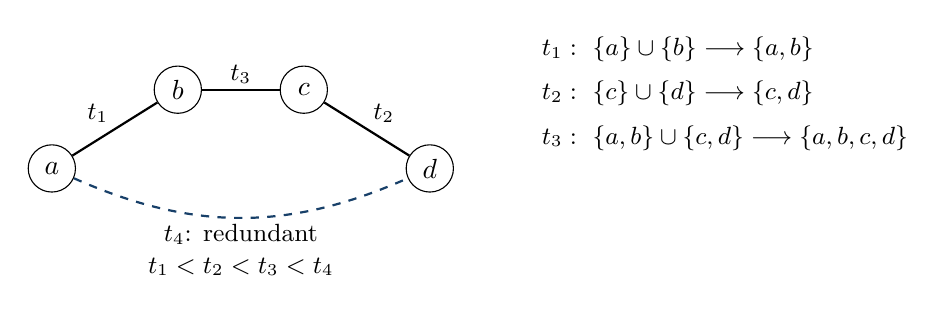
\begin{tikzpicture}[x=1cm,y=1cm,
  particle/.style={circle,draw=black,fill=white,minimum size=6mm,inner sep=1pt},
  merger/.style={thick},
  extra/.style={thick,dashed,draw=linkblue},
  lab/.style={font=\small,fill=white,inner sep=2pt}]
 \node[particle] (a) at (0,0) {$a$};
 \node[particle] (b) at (1.6,1) {$b$};
 \node[particle] (c) at (3.2,1) {$c$};
 \node[particle] (d) at (4.8,0) {$d$};
 \draw[merger] (a)--node[lab,above left] {$t_1$}(b);
 \draw[merger] (b)--node[lab,above] {$t_3$}(c);
 \draw[merger] (c)--node[lab,above right] {$t_2$}(d);
 \draw[extra] (a) to[bend right=24]
    node[lab,below] {$t_4$: redundant}(d);
 \node[anchor=west,font=\small,align=left] at (6.1,.95)
   {$t_1:\ \{a\}\cup\{b\}\longrightarrow\{a,b\}$\\[5pt]
    $t_2:\ \{c\}\cup\{d\}\longrightarrow\{c,d\}$\\[5pt]
    $t_3:\ \{a,b\}\cup\{c,d\}\longrightarrow\{a,b,c,d\}$};
 \node[font=\small] at (2.4,-1.25) {$t_1<t_2<t_3<t_4$};
\end{tikzpicture}
\caption{Chronological connectivity for four particle lines. Each solid
contact joins two previously separate components and fixes one relative
translation, with the incoming-flux Jacobian \(\eps^2B\,\dd t\,\dd\omega\).
The dashed contact is internal to the already joined component. Its
relative position is fixed, so it contributes a constraint rather than a
new translation variable. Later common translations cannot change that
constraint. Edges depict the contact graph, not physical trajectories.}
\label{fig:chronological-mergers}
\end{figure}

The distinction between a new merger and a redundant contact is
illustrated in \Cref{fig:chronological-mergers}.  It refers to the
chronological connected components of the contact graph, not to spatial
proximity at an unspecified time.

\begin{lemma}[Chronological merger coordinates]\label{lem:sharp-merger-coordinates}
Fix a finite line graph, the C/O choices, the chronological order, and
which contacts are redundant in that order.  Away from nontransversal
contacts and simultaneous events, its history integral has coordinates
consisting of the birth velocities, one absolute translation for each
global component, a vector in a ball of radius \(R_{K,D}\eps\) for each
physical initial merger, and
\((t,\omega)\in\R\times S^2\) for each dynamic merger.  The positional
Jacobian at a dynamic merger is
\begin{equation}\label{eq:sharp-jacobian}
       \eps^2[(v-v_*)\cdot\omega]_+\,\dd t\,\dd\omega.
\end{equation}
A specified redundant contact has no free continuous parameter and
requires no extra Jacobian.  The coordinate map has multiplicity at most
one on each prescribed incoming straight-segment branch.
\end{lemma}

\begin{proof}
Choose the birth velocities first.  Initially every line has an
independent translation of its free affine trajectory.  An initial
forest link determines the difference between the translations of its
two groups by a vector in the stated ball.  Orient the forest toward
one representative per group.  The changes from individual translations
to representatives and these differences have determinant one.

Proceed in increasing contact time.  Inductively, the histories within
each group have been constructed, including all velocity changes before
the next merger, and are known up to a common translation of that group.
For a merger between groups with translations \(X\) and \(X_*\), the
contact condition on the indicated straight segments is
\[
 X-X_*=-d(t)-\eps\omega,
\]
where \(d(t)\) is the known relative displacement with the translations
removed, and \(\omega\) is opposite to the outward geometric relative
normal.  Thus incoming contact has \((v-v_*)\cdot\omega>0\), as in
\eqref{eq:collision-kernel}.  On these segments
\(\dot d(t)=v-v_*\).  The determinant of
the map from time and surface coordinates on \(S^2\) to \(X-X_*\) is
\(\eps^2|(v-v_*)\cdot\omega|\).  The incoming convention selects the
sign in \eqref{eq:sharp-jacobian}.  A scattering contact applies the
elastic velocity reflection; an O contact retains the velocities.  The
two groups now have one common free translation.

If the next specified contact is redundant, its relative displacement
and velocities on the indicated segments are already fixed.  A straight
relative trajectory has at most one incoming intersection with the
sphere of radius \(\eps\).  More precisely, for its relative flight
\(r(t)=d+tu\) on the common segment interval \(I\),
\[
 \int_I\delta(|r(t)|-\eps)
       [-u\cdot r(t)/\eps]_+\,\dd t
 =\ind_{\{\text{an incoming intersection occurs in }I\}}.
\]
At a transversal incoming crossing, the flux cancels the absolute
derivative of \(|r(t)|-\eps\).  The outgoing delta factors then make
the prescribed C or O substitution.  Thus its time and normal, when
the prescribed intersection exists, are determined.  If it does not exist, the branch
has weight zero.  This includes segments starting inside the sphere:
their outgoing exit is not an incoming intersection.  Subsequent
translations of the entire group leave this test and its resulting
velocity reflection unchanged.

Every step therefore uses only coordinates fixed at earlier steps.  Its
derivatives with respect to those earlier coordinates may be nonzero,
but the full determinant is triangular and is the product of the
displayed diagonal determinants.  There is no new unknown relative
translation at a redundant step.  Contacts at different birth interfaces
are treated identically: the affine origins of the new lines differ,
but the derivative of their current displacement is still their current
velocity.  At the end retain one representative translation per global
component.  On an incoming transversal branch the reverse construction
recovers every relative translation, so the multiplicity is one.

For a finite graph the excluded segment boundaries, equality of two
specified times, and zero incoming flux have measure zero in merger
coordinates unless they belong to a redundant-contact requirement.
Such a requirement is retained as an indicator; no change of variables
is performed at it.  Equivalently, one may first work on compact subsets
of the transversal branches and then exhaust them.  This also justifies
the formula for nonnegative history integrals without smooth densities.
\end{proof}

Multiplying \eqref{eq:sharp-activity} by the merger Jacobians and the
physical link volumes gives
\begin{equation}\label{eq:sharp-scaling}
 \mu^{m-h}\eps^{2(m-c-p)}\eps^{3p}
                     =\mu^{c-h}\eps^p.
\end{equation}
All history acceptance indicators can be retained during the coordinate
change.  For an upper bound they can subsequently be dropped, except
that a redundant scattering is used to determine the velocities of its
specified branch when it occurs.  Dropping the requirement of its
occurrence is understood as extending the resulting integrand by zero
off that branch, not as assigning an arbitrary additional velocity.

For a connected diagram \(c=1\).  A nontrivial physical initial block
has \(p\ge1\), and thus gains at least one factor \(\eps\).  If a term
in \eqref{eq:sharp-initial-link} instead uses a tail factor, erase that
link.  Erasing at most \(K\) links increases the number of components
by at most \(K\), and the extra activity cost in
\eqref{eq:sharp-scaling} is at most \(\eps^{-2K}\).  Choosing
\(D>2K+M\) makes the terms with at least one such tail
\(O(\eps^M\mu^{1-h})\).  Here \(M\) is arbitrary and is chosen after
the required moment order.  The constants in a physical link radius
and the forest count involve only boundedly many links.

\subsection{Factorials and a summable majorant}

\begin{lemma}[The fresh-label factorials]\label{lem:sharp-factorials}
For diagrams of complexity at most \(K\), the absolute sum with slab
sizes \((n_1,\ldots,n_L)\) is bounded by a sum over chronologically
ordered merger pair lists with denominator \(\prod_i n_i!\), multiplied
by
\begin{equation}\label{eq:sharp-polynomial-count}
 C_K(1+n)^{d_K}C^{\sum_i a_i},
 \qquad n=\sum_i n_i,
\end{equation}
where the base \(C\) does not depend on \(K\).  The merger pairs
themselves are not counted in \eqref{eq:sharp-polynomial-count}.
\end{lemma}

\begin{proof}
In slab \(i\), let \(s_i\) be the number of labels arriving as roots
from above, including the final designated roots in the highest slab.
The finite factorial expansion integrates \(j_i=n_i-s_i\) new labels
with coefficient \(1/j_i!\).  Since \(s_i\le K\),
\[
 \frac1{j_i!}=\frac{n_i!}{(n_i-s_i)!}\frac1{n_i!}
             \le\frac{(1+n_i)^{s_i}}{n_i!}.
\]
The choices of continued labels, dependent subsets, and labels in
initial links all involve boundedly many labels; their number is a
fixed power of \(1+n\).

The rooted compatibility expansion in \Cref{thm:marked-expansion}
represents each connected cluster coefficient by spanning forests.
Its deterministic exploration gives at most one branch per selected
forest.  After selecting an incoming encounter for each chosen forest
edge, the C components are exactly the isolated collision clusters;
the O forest specifies their blocks.  Consequently these partitions
are recovered from the C/O graph and do not furnish a further partition
factor.  The retained unexpanded independent factors and the continued
labels specify the lower-slab attachment.  This is also why taking a
tree bound for a compatibility coefficient does not remove the
fresh-label denominator.

There are at most \(r\le C_K\) redundant contacts.  Their ordered pair
labels cost at most \((1+n)^{2r}\), and inserting them among the merger
contacts costs at most \((1+n+r)^r\).  Initial forests and the choices
of the bounded exceptional labels have the same polynomial form.
Each ordinary contact has at most two C/O flags, which gives an
absolute exponential base.  A chronological order already determines
the order of contacts on every line; it has no separate permutation
factor.  These observations give
\eqref{eq:sharp-polynomial-count}.  The bounded exceptional counts
alter \(C_K,d_K\), not the base multiplying each ordinary merger.
\end{proof}

\begin{lemma}[Uniform summability]\label{lem:sharp-summability}
For fixed \(K\), the sum of the absolute connected diagram measures
with slab sizes \((n_i)\), after removal of the factor
\(\mu^{1-h}\), is bounded by
\begin{equation}\label{eq:sharp-summable}
       C_K(1+n)^{d_K}(C\tau\sqrt L)^n.
\end{equation}
The same bound, with the appropriate factor \(\mu^{c-h}\), holds
after a bounded number of initial links are erased.  It also holds
after prescribing the absolute spatial position of one observation
in each component, or after inserting a sufficiently small Gaussian
weight in the designated velocities.
\end{lemma}

\begin{proof}
We give the energy and time estimates jointly, to avoid putting a
separate logarithmic velocity loss at each vertex.  Let
\(E_0=\sum_{p=1}^m|v_p^{\mathrm{birth}}|^2\).
Elastic collisions conserve the energy of each colliding pair, O
contacts do not change it, and a line ending at an interface discards
its energy.  Introducing a birth adds the energy already included in
\(E_0\).  Hence the sum of squared velocities of all lines active at
any time is at most \(E_0\).

On the bin \(E_0\in[P/2,P]\), with the bin \(E_0<1\) included by
using \(P=1\), the one-step sum of incoming speed factors over all
choices of a merger pair in slab \(i\) satisfies
\begin{equation}\label{eq:sharp-pair-flux}
 \sum_{p<q}|v_p-v_q|
 \le (n_i-1)\sum_p|v_p|
 \le n_i^{3/2}\sqrt P.
\end{equation}
This estimate is applied to a discrete tree of successive pair
choices at fixed merger times, normals, and birth velocities.  At a
node, all earlier velocities and all intervening specified redundant
contacts are already determined by
\Cref{lem:sharp-merger-coordinates}.  The sum of the weights of its
children is bounded by \eqref{eq:sharp-pair-flux}; an unrealizable
child contributes zero.  Induction over that discrete tree bounds
the sum of the products of fluxes by
\begin{equation}\label{eq:sharp-pair-products}
                  \prod_i(n_i^{3/2}\sqrt P)^{a_i}.
\end{equation}
Integrating the normals adds \(C^{\sum_i a_i}\).  The merger times
are globally ordered within each slab, even if some redundant times
are inserted between them.  Dropping further constraints leaves
time volume at most \(\prod_i\tau^{a_i}/a_i!\).

There remains a common translation for each component.  For any
fixed birth velocities and merger coordinates, write the spatial
arguments of its inputs as \(X+d_p\).  Integrate one chosen input
in \(X\) and use the spatial supremum of every other input.  The
Bol norms in \eqref{eq:sharp-input-bounds} give a factor at most
\(C^m\exp(-bE_0)\).  This bound is independent of the displacements
\(d_p\), which can be large.  To prescribe an observation position
instead, solve \(X=x-d_{\mathrm{obs}}\) and use a spatial supremum
for every input.  The Jacobian is one and the same Gaussian bound
holds uniformly in \(x\).

We spell out the velocity-volume step.  By reserving half of the
Gaussian suppression, for a suitable \(b_1>0\),
\[
 \ind_{E_0\in[P/2,P]}e^{-2b_1E_0}
       \le e^{-b_1P/2}e^{-b_1E_0}.
\]
The integral of the last factor over the \(3m\) birth velocity
coordinates is \((\pi/b_1)^{3m/2}\).  On the lowest bin \(E_0<1\),
omit the dyadic suppression factor and use \(P^{a/2}=1\);
integrating the reserved Gaussian still costs only \(C^m\).
Thus no uncounted power of the energy-bin volume remains.
If \(a=\sum_i a_i\), summing the
dyadic energy bins yields
\begin{equation}\label{eq:sharp-energy-sum}
 \sum_{P=1,2,4,\ldots} e^{-b_1P/2}P^{a/2}
                    \le C^{a+1}(1+a)^{a/2}.
\end{equation}
For example, comparison with the integral of
\(e^{-b_1u/4}(1+u)^{a/2}\) proves this by the gamma integral and
Stirling's inequality.  Its constant depends on \(b_1\), not on
\(K\).

Combining these estimates with \Cref{lem:sharp-factorials}, the
remaining quantity is bounded by a fixed polynomial in \(1+n\)
times
\begin{equation}\label{eq:sharp-before-stirling}
 C^{n+a}\tau^a(1+a)^{a/2}
            \prod_i\frac{n_i^{3a_i/2}}{a_i!n_i!}.
\end{equation}
Set \(\delta_i=n_i-a_i\).  By
\eqref{eq:sharp-line-count}, \(\delta_i\ge0\) and
\(\sum_i\delta_i\le C_K\).  The inequalities
\(n_i!/a_i!\le(1+n_i)^{\delta_i}\) and
\(n_i!\ge(n_i/e)^{n_i}\) imply
\[
 \frac{n_i^{3a_i/2}}{a_i!n_i!}
 \le e^{2n_i}(1+n_i)^{\delta_i}n_i^{-n_i/2},
\]
where zero counts contribute one.  Also
\(\tau^a\le\tau^n\max(1,\tau^{-1})^{C_K}\), and
\((1+a)^{a/2}\le C(1+n)^{C_K}n^{n/2}\), after adjusting the
bounded-size cases.  Finally convexity of \(u\log u\) gives
\begin{equation}\label{eq:sharp-layer-entropy}
               \prod_i n_i^{n_i}\ge(n/L)^n.
\end{equation}
Substitution in \eqref{eq:sharp-before-stirling} proves
\eqref{eq:sharp-summable}.

At a fixed time the sum of squared designated velocities is at
most \(E_0\).  At \(q_0\) record times their total is at most
\(q_0E_0\).  A weight with exponent smaller than
\(b_1/(2\max(1,q_0))\) can therefore be absorbed in the Gaussian
factor reserved above.  This proves the weighted assertions.  The
exponent is chosen so that the fraction of birth Gaussian reserved
for all record times together is fixed; the exponential base
therefore does not grow with the number of observations.  The powers
supplied by initial physical links
and erased links are those already computed in
\eqref{eq:sharp-scaling} and do not affect the summation argument.
\end{proof}

Since \(\tau=T/L\), the base in \eqref{eq:sharp-summable} is
\(CT/\sqrt L\).  Increase \(L\) once so it is less than one.
The number of vectors \((n_i)\) of total size \(n\) is a polynomial
in \(n\), since \(L\) is fixed.  Thus
\eqref{eq:sharp-summable} proves uniform summability and uniform
vanishing of the size tails for every fixed \(K\).  Polynomial
degrees may grow with the factorial order; this never requires
another enlargement of \(L\).

\subsection{The extra-contact null sets}

We next prove the qualitative geometric fact needed for cycles.
Only a fixed finite graph is considered in this subsection.  All
birth velocities, contact times, merger directions, and one free
translation per component are its independent parameters.  They carry
a measure absolutely continuous with respect to the product of
Lebesgue measure and surface measure.  An assertion concerning lines
within the same connected component is invariant under its common
translation and remains valid when one observation position in that
component is fixed as in \Cref{lem:sharp-summability}.  No conditioning
on additional positions or velocities is used in the null-set argument.

\begin{lemma}[No extra contact for a limiting tree]\label{lem:sharp-no-extra}
Consider a finite chronological forest with no physical initial
links, with a prescribed C/O choice on each edge, on its incoming
merger branches.  Outside a null set of its merger parameters the
following hold.
\begin{enumerate}[label=(\roman*)]
\item All specified contacts occur at distinct times away from
interfaces and observation times and are transversal.
\item Before the first redundant contact, the demand for such a
contact is false for all sufficiently small \(\eps\).
\item On a full tree, an additional contact not in the prescribed
list, including a contact preceding the prescribed joining of its
two groups, is absent for all sufficiently small \(\eps\).
\end{enumerate}
In (ii), the independent parameters used are those of the forest
prefix; arbitrary remaining merger parameters may be appended.
In (iii), an outgoing crossing following an O contact is not an
additional contact, because only incoming crossings are counted.
\end{lemma}

\begin{proof}
For clarity first set \(\eps=0\) in the formal trajectories.  At
each prescribed C contact the velocities are transformed by the
linear reflection of the pair velocity in its contact direction;
at an O contact they are unchanged.  Every segment velocity is
therefore polynomial in the birth velocities and in the coordinates
of the sphere directions.  A segment displacement is polynomial
also in the prescribed times.  The parameters lie on the connected
real analytic manifold given by the product of their Euclidean
spaces, the spheres, and an open time simplex.  Consequently a
polynomial expression that is not identically zero has a null zero
set.  It is legitimate to use grazing or ineffective reflections
to test nonidentity: the reflection formulas extend analytically
to those parameters, although the physical flux there may vanish.

There are finitely many pairs of lines and finitely many pairs of
their straight segments.  On a common time interval write their
relative displacement as \(d+tu\).  A coincidence on this interval
requires
\begin{equation}\label{eq:sharp-collinearity}
                             d\times u=0.
\end{equation}
We check the only cases in which this condition could be forced.
If the two lines belong to different forest components, variation
of their free relative translation disproves the identity
\eqref{eq:sharp-collinearity} immediately.  The assertions used for
the first redundant contact and for a connected full tree concern
lines in the same component, as treated next.

Suppose first that the lines are not neighbors in the prescribed
tree.  Make all reflections ineffective.  If the unique joining
path is \(p_0,p_1,\ldots,p_k\), \(k\ge2\), with its edge contact
times \(s_1,\ldots,s_k\), then solving the contact equations gives
the endpoint displacement as a sum of terms
\((v_{p_{j-1}}-v_{p_j})s_j\), plus the endpoint free-flight term.
For \(1\le j<k\), the independent velocity \(v_{p_j}\) occurs
with coefficient \(s_{j+1}-s_j\), up to an immaterial common sign.
These two times are distinct.  Set the endpoint relative velocity
nonzero and vary this intermediate velocity in a direction not
parallel to it.  This disproves the identity
\eqref{eq:sharp-collinearity}.  Branches off the path and birth
interfaces do not alter this test: ineffective reflections leave
their velocities unchanged, and birth times only alter the affine
origins solved for by the contact equations.

Suppose next that the two lines are neighbors and have their
prescribed meeting at time \(a\).  On segments after \(a\), if
neither endpoint has subsequently changed velocity, their flight
is the single separating relative flight from that meeting.  It
cannot give a second incoming crossing, either at zero diameter
or at positive diameter.  This includes an O contact: its relative
flight passes through the sphere and exits once, but does not
enter it a second time without a velocity change.

If an endpoint has a subsequent scattering at time \(b\), take
the first effective such scattering in testing nonidentity and
make all other reflections ineffective.  Its third particle is
distinct from the original pair, since another edge between that
pair would form a cycle.  With all other reflections ineffective,
this third particle's current velocity equals its independent birth
velocity, even if it has a prescribed earlier history.  One can choose
this velocity and the scattering normal so that the relative
velocities of the original pair before and after \(b\) are two
nonparallel vectors \(u_1,u_2\).  Their displacement on the later
segments then contains
\[
                   (b-a)u_1+(t-b)u_2.
\]
Its cross product with \(u_2\) is nonzero, since \(b\ne a\).
For an explicit choice, keep the untouched endpoint at velocity
zero, take the other endpoint's velocities to be \(e_1\) before
and \(e_2\) after the scattering, and use a third-particle velocity
\(-e_1\) with normal \((e_1-e_2)/\sqrt2\).  The equal-mass
reflection gives the stated outgoing endpoint velocity.  This
again disproves \eqref{eq:sharp-collinearity}.  For a segment before
the neighboring pair's prescribed meeting, choose an intervening
scattering time \(b<a\) with the same change from \(e_1\) to
\(e_2\).  Before \(b\), the relative displacement required to
meet at \(a\) is
\[
                 (t-b)e_1-(a-b)e_2,
\]
which is not parallel to the segment relative velocity \(e_1\).
With no intervening reflection the earlier relative flight has
only its prescribed incoming crossing.  This proves the
earlier-segment case without any condition on time-reversed
feasibility.

These arguments use the entire tree and therefore also exclude an
unintended earlier contact between groups whose relative translation
is fixed only by a later prescribed merger.  For a first required
redundant contact, they need only the joining tree in the prefix:
the two lines are already in the same group, and all their relative
parameters are fixed there.  Adding parameters belonging to the
rest of the graph preserves a null exceptional set by Fubini's
theorem.

Zero relative velocities and grazing prescribed contacts have
null parameter sets.  Indeed the incoming relative velocity at a
merger is the difference of velocities from two disjoint previous
groups; it is not an identically zero linear function of their
independent birth velocities.  The normal is a free sphere
parameter.  Specified time coincidences, including equality with
an interface or an observation time, have null time measure.  A
third line at a prescribed vertex has no forced coincidence:
at least one of its paths to the two incident lines is a
nonneighbor path, to which the intermediate-velocity argument
applies.  Endpoints of line lifetimes at interfaces are treated
by the same finite-segment test.  We discard this finite union of
null sets.

It remains to justify that an absent zero-diameter coincidence
excludes positive-diameter contacts, particularly contacts converging
to a prescribed vertex.  For fixed merger times, directions, and
birth velocities the formal tree velocities do not depend on
\(\eps\).  Write each line as
\(x_p(t)=X_p+Y_p(t)\), with \(Y_p\) determined by its velocities.
The edge equation is
\[
 X_p-X_q=-\eps\omega_{pq}-Y_p(s_{pq})+Y_q(s_{pq}).
\]
Solving these equations along the forest shows that, after fixing
its representative translations,
\begin{equation}\label{eq:sharp-uniform-tree-convergence}
        x_p^\eps(t)=x_p^0(t)+\eps d_p,
\end{equation}
where each \(d_p\) is a fixed finite sum of merger normals.
Thus convergence is uniform on every active line interval.

Away from small neighborhoods of the finitely many prescribed
vertices, every pair of closed straight-segment pieces either
has a strictly positive minimal separation or is the already
treated separating flight of a neighboring pair.  For sufficiently
small diameter no new contact can occur there.  Near a prescribed
vertex, a different pair would require an additional zero-offset
pair coincidence, already excluded by the finite-segment argument.
This includes a third-particle coincidence at that vertex and a
disjoint pair coinciding elsewhere at the same time.  The incident
pair has no other velocity
change in a sufficiently small fixed neighborhood, because all
event times are distinct.  It has only the one prescribed incoming
crossing on that neighborhood.  In particular two incoming
crossings cannot collapse onto that vertex.  The same compactness
argument applies to interfaces and observation times.  This proves
(ii) and (iii), including contacts whose times vary with \(\eps\).
\end{proof}

For a graph containing a cycle, keep its first redundant-contact
indicator.  All preceding contacts form a forest, and the relative
trajectory tested by this indicator is determined by that forest
prefix.  No later redundant-contact velocity update enters this test.
By \Cref{lem:sharp-no-extra} it tends to zero for almost
every choice of the independent parameters preceding that contact.
After a finite size truncation, velocities and representative
translations can first be truncated as well.  On those compact
sets the integrands after \Cref{lem:sharp-merger-coordinates} have
an integrable bound, obtained either directly from the finitely
many speed factors or from the proof of
\Cref{lem:sharp-summability}.  One can extend an unrealizable
branch by zero.  Dominated convergence therefore makes the
scaled absolute integral tend to zero.  The velocity and spatial
truncations are then removed by the Gaussian bounds and the uniform
spatial tightness supplied by the Bol-norm convergence in
\eqref{eq:sharp-input-bounds}, and
finally the size truncation is removed using
\eqref{eq:sharp-summable}.  This order of limits needs no rate
uniform in the number of vertices.  Together with
\eqref{eq:sharp-scaling}, it proves the asserted little-o for
cycles and nontrivial initial cumulants.

\subsection{Tree convergence and spatial disintegration}

For a fixed tree all its prescribed C-clusters and O blocks are
below their cutoffs once \(\eps\) is small.  By
\Cref{lem:sharp-no-extra}, almost every set of merger parameters
has only the prescribed incoming contacts for all sufficiently
small \(\eps\).  Thus all history acceptance restrictions then
hold, and counting a selected encounter instead of its existence
changes nothing.  The connected compatibility coefficient on
this configuration is exactly its tree sign \((-1)^{\#O}\).
There is no nontrivial initial link.  The changes of relative
translations therefore leave precisely the fluxes in
\Cref{thm:sharp-cumulants}, after multiplication by
\(\mu^{h-1}\).

Replacing each \(g_i\) by \(f_{i\tau}\) in a fixed-size term is
justified by a telescoping product and
\eqref{eq:sharp-input-bounds}.  The proof of
\Cref{lem:sharp-summability}, with one of the factors replaced by
its Bol-norm difference, gives convergence to zero for that
difference.  For these continuous limiting inputs,
\eqref{eq:sharp-uniform-tree-convergence} and the absence of
contacts at observation times give convergence of every bounded
continuous record test.  The remaining dominated convergence in
spatial translations can be checked first on bounded velocities
and bounded size.  On that set the relevant input displacements
are bounded; the summable cell envelopes in the Bol norm control
the spatial tails uniformly.  Then use
\Cref{lem:sharp-summability} to remove the truncations.  This
defines the limiting signed tree measures.

\begin{lemma}[Spatial traces of tree measures]\label{lem:sharp-spatial-traces}
Let \(\mathcal T\) be any of the absolutely summable tree measures
just constructed, and designate a line and a time at which its
position is required.  It has a version of the disintegration
\begin{equation}\label{eq:sharp-disintegration}
               \mathcal T=\dd x\,\mathcal T_x
\end{equation}
with respect to that position.  For a sufficiently small
\(\alpha>0\), the Gaussian-weighted variation of
\(\mathcal T_x\) is bounded uniformly in \(x\); its integral over
\(x\) is finite.  For every bounded continuous test of the other
coordinates, and also for continuous tests of smaller Gaussian
growth, \(x\mapsto\mathcal T_x(\Phi)\) is continuous.

If two separate tree components are joined at their designated
positions, the product of their conditional measures at a common
position, integrated against incoming flux, is an absolutely
defined measure.  It is the result of imposing the joining
position in the merger coordinates.  Equivalently it is obtained
by a smooth approximate identity for equality of the two
positions.  These facts apply to the marked one-root and
connected two-root tree measures and their record projections.
\end{lemma}

\begin{proof}
For a finite tree choose its free representative translation to
be the position \(x\) of the designated observation.  Every
birth position is then \(x+d_p\), and every recorded position
has the same form, with displacements independent of \(x\).
The derivative in the representative translation is the identity.
This constructs \eqref{eq:sharp-disintegration} as an actual
integral formula, not just as an almost-everywhere equivalence
class.  The fixed-position and integrated versions of
\Cref{lem:sharp-summability} give both asserted variation bounds.

After truncation in size and velocity, the integrand against a
continuous record test is continuous in \(x\), by continuity of
the limiting inputs and the observation updates.  It has the
same integrable majorant uniformly for \(x\) in a compact set.
The velocity tails and the graph-size tails converge uniformly
in \(x\), by the fixed-position estimate.  This proves the
stated continuity.  Gaussian growth in the test is handled by
reserving a slightly stronger Gaussian weight first.

Let the designated variables in two different components have
positions \(x,x_*\).  Their joint integral before joining uses
two independent translations and the product measure.  Setting
\(x_*=x\) gives the claimed conditional product.  The bound
\(B(v-v_*,\omega)\le |v|+|v_*|\), with a slight Gaussian
exponent loss, makes its variation finite: use the uniform
conditional bound for one component and the integrated bound
for the other.  The same estimate dominates a compactly
supported smooth approximate identity in \(x-x_*\), uniformly
in its width.  On bounded velocity sets conditional weak
continuity implies convergence of the product measures against
continuous tests; products of continuous single-component
tests suffice first, and their finite sums approximate a
continuous test on each compact set.  The Gaussian and spatial
variation bounds then remove the compact truncations.  This
proves the approximate-identity characterization and its
agreement with merger coordinates.  Forgetting records commutes
with every displayed integral.
\end{proof}

\subsection{Completeness and splitting of the retained trees}

The preceding size limit was taken with bounded complexity.  It
is necessary to verify that a fixed sufficiently large complexity
cutoff includes every leading tree allowed by the regrouping rule,
even though it may have arbitrarily many ordinary vertices.

\begin{lemma}[Completeness of the tree class]\label{lem:sharp-tree-completeness}
For fixed designated roots, fixed required records, and fixed
\(L\), all global trees with trivial initial cumulants in the
retained expansion after the one-root regrouping of
\Cref{lem:marked-regrouping} have complexity at most a fixed constant
\(K_0\).  This bound is independent of their number of ordinary
contact vertices.  Undoing and reapplying an unmarked one-root
regrouping preserves their weights and their record projections.
\end{lemma}

\begin{proof}
We first prove that an unmarked dependent one-root component
cannot be a tree with trivial initial cumulants.  In its highest
occupied slab, a one-root component has a single connected
block.  If all lower inputs of this block are independent, it
is precisely a term in the definition of \(g_i\), and is
regrouped into that independent factor.  If a connected lower
dependent component attaches to the block through two lines,
the upper connection between these lines and their lower
connection form a global cycle.  For a global tree, every
lower dependent component therefore attaches through at most
one line.  At least one such component must exist for the
upper one to remain dependent.  Following it downward repeats
the same argument on a smaller number of slabs.  At time zero
there is no dependent singleton, and a dependent nonsingleton
requires a nontrivial initial cumulant.  This contradiction
proves the claim by downward induction.  Required records are
the only reason to expand an otherwise independent singleton
history further.

Now cut a global forest at an interface and contract each of
its upper components to a vertex.  Suppose there are \(u\)
such vertices.  A lower connected component with \(k\ge2\)
attachments cannot touch the same upper component twice, since
that creates a cycle.  The bipartite incidence graph of these
lower components and the upper vertices is a forest.  If there
are \(v\) lower vertices of degree at least two and \(d\)
incidence edges, then \(d\le u+v-1\) in each nonempty connected
part, while \(2v\le d\).  In particular
\begin{equation}\label{eq:sharp-crossing-bound}
                               d\le 2u.
\end{equation}
A lower component attached at a single line either is absorbed
into an independent input, by the first paragraph, or continues
a required record.  The latter contribute at most the fixed
number of recorded lines at that interface.  Empty continued
lines are included in this count.

Starting with the fixed number of final roots and iterating
\eqref{eq:sharp-crossing-bound} through \(L\) slabs therefore
bounds the total number of interface roots and recorded
singleton continuations.  There are no cycle or initial-link
contributions to complexity in a leading tree.  This gives
\(K_0\).  The argument applies separately to disconnected
expressions and to projections with fewer required records.

Regrouping an unmarked one-root component is the defining
finite sum for its independent factor, with its original
fresh-label coefficient.  Its components attach at one line
only.  Thus undoing it neither changes a connection between
different remaining components nor introduces a constraint
between them.  The exact finite identity in
\Cref{thm:marked-expansion} shows that forgetting records and
regrouping commute before a limit.  Absolute summability from
\Cref{lem:sharp-summability} gives the same identity for the
limiting trees.  Their weights and projections are therefore
preserved.
\end{proof}

\begin{lemma}[Last-contact products]\label{lem:sharp-tree-splitting}
In the leading tree sums, deleting a last contact of the highest
slab that meets a designated root splits its global tree into
the product of the two component tree measures, with the
incident lines designated before that contact.  Their product
at the collision position is the conditional product in
\Cref{lem:sharp-spatial-traces}.  Conversely, joining such two
disjoint component histories at that contact gives exactly
the corresponding retained tree, with its original factorial
weight.  Record portions not used by a test are projected out.
These operations are valid for bounded continuous record tests
and, with a smaller exponent, for tests of Gaussian velocity
growth.
\end{lemma}

\begin{proof}
Temporarily expand all independent factors in the highest slab by
their one-root definitions for that slab, retaining their lower inputs
in the canonical regrouped form.  Bound the total number of lines in
each resulting limiting tree by \(N\).
For sufficiently small \(\eps\), every particle cap \(\Lambda_i\)
and retained cluster cap \(M_i\) exceeds \(N\).  The convergence
already proved therefore supplies every such leading tree with its
original factorial weight.  We perform the following finite algebra
on this limiting tree class, preserving the inherited bound on the
combined size after a split.  This is not a claim that arbitrary
finite-\(\eps\) capped classes are closed under joining.

Deleting an edge of a global tree makes exactly two components.
Each contains one incident
line of the deleted contact, which is now designated.  If a
component in the highest slab loses its old designated root,
it contains the newly designated incident line or another
original root.  Thus it still satisfies the rooted-block rule.
All lower attachments are unchanged.  They can be put in the
canonical retained form by the singleton regrouping of
\Cref{lem:sharp-tree-completeness}.

Conversely, the two components are disjoint before joining.
Adding their incident edge creates a tree, and its highest
block meets the original root.  The inverse singleton
regroupings restore precisely its retained representation.
This is a bijection at the level of the temporarily expanded
labelled trees.  In particular it is not a factorization of
the actual particle law at an interface.

For the coefficients, choosing an additional incident particle
among \(j\) fresh labels changes \(1/j!\) into
\(1/(j-1)!\).  If the remaining fresh labels are divided into
sets of sizes \(j_1,j_2\), their distribution contributes the
binomial coefficient satisfying
\[
 \binom{j_1+j_2}{j_1}\frac1{(j_1+j_2)!}
                          =\frac1{j_1!j_2!}.
\]
Apply this identity in each slab.  A contact between two
already designated particles uses their single unordered
pair; it has no fresh-label factor.  The sign of the deleted
contact is its C/O sign, and all other signs multiply over
the two components.  This proves the coefficient assertion.

The finite identities retain the combined-size restriction just
specified.  Letting \(N\) increase removes that restriction and
passes the sums through the deletion and joining integrals by
\Cref{lem:sharp-summability,lem:sharp-spatial-traces}.  The
uniform conditional Gaussian bound controls the velocity
flux introduced by the join, with a fixed exponent loss.
Record projection commutes with the finite hierarchy and
with the one-root regrouping, as established above.  Hence
a temporarily designated partner for which no past record
appears in the integrand requires only the projected
component measure.  Approximation locally uniformly with
a stricter Gaussian exponent extends the identity to the
stated test class.
\end{proof}

\begin{proof}[Proof of \Cref{thm:sharp-cumulants}]
We first justify weighted control of the retained high-complexity
tail.  Choose the common birth exponent \(b>0\) in
\eqref{eq:sharp-input-bounds} independently of \(L\), and choose
\(L\) large enough for the coarse package with the fixed smaller
exponent \(3b/4\) as well.  For a fixed observation list let \(J\)
be the number of designated endpoint and record velocity slots.
On every original retained history, conservation of energy gives
\[
 \sum_{\text{these slots}}|v|^2\le J E_0.
\]
Choose the weight exponent \(\alpha>0\) with \(\alpha J\le b/4\).
Its Gaussian weight is dominated by \(e^{bE_0/4}\), which can be
absorbed by replacing every absolute birth input \(|g_i(x,v)|\)
or \(f_0(x,v)\) by that input times \(e^{b|v|^2/4}\).
The resulting inputs have a common \(\Bol,3b/4\) bound.
The positive coarse estimate in \Cref{thm:dhm-package}(a)
requires this envelope, not closeness to the Boltzmann solution.
Apply it to the tilted inputs, with the same initial-link and
fixed-record bounds used in \Cref{thm:marked-expansion}.
Dummy inputs, if used for that bound, may be tilted too;
their additional birth energy only enlarges the majorant.
The same geometric complexity sum makes the weighted retained
tail smaller than any assigned power of \(\eps\), after choosing
\(K\) for the fixed order and accuracy.  The Gaussian fraction
reserved here is fixed, so its atom base does not depend on
\(J,h,K\).  Only the observable weight exponent decreases with
the record list.  This argument concerns retained diagrams,
not a microscopic expansion remainder.

Use \Cref{thm:marked-expansion} with an accuracy
\(\eps^M\) where \(M>2(h-1)\), and with a complexity cutoff
large enough both for that accuracy and for
\Cref{lem:sharp-tree-completeness}.  The expansion error and
the high-complexity tail are negligible after multiplication
by \(\mu^{h-1}\).  They need only their unweighted variation
bound, because the observation tests here are bounded.

For the remaining connected diagrams,
\eqref{eq:sharp-scaling} and
\Cref{lem:sharp-summability} prove the uniform bound at scale
\(\mu^{1-h}\).  Physical initial links gain \(\eps\);
nonphysical initial tails gain any assigned power after
choosing \(D\) as above.  Cycles are negligible by
\Cref{lem:sharp-no-extra}, finite-size dominated convergence,
and the uniform size tails.  The diagrams that remain are
the complete class of leading trees, by
\Cref{lem:sharp-tree-completeness}.  Their fluxes, signs,
input limits, and continuous record tests were evaluated
above.  The same summable majorant proves the asserted
Gaussian variation bounds for their retained sums and
their limits.  In particular it gives the one-root and
two-root limits needed in the next section.  All exponential
bases used in this proof are independent of \(K\) and of
the fixed order \(h\); dependence on those quantities occurs
only in front constants and polynomial degrees.  Thus the
choice of \(\Gamma,L\) remains the single choice made before
the moment order was specified.
\end{proof}

\section{Identification of the covariance and the Gaussian limit}
\label{sec:gaussian-limit}

Fix a finite observation list and absorb the coefficients of any desired
real linear combination into its tests \(\phi_j\).  We first prove the
Gaussian limit for the single pasted dynamics supplied by
\Cref{thm:marked-expansion,thm:sharp-cumulants}.  Its parameters
\(\Gamma,L\) do not depend on the observation list or a moment order;
only auxiliary complexity and initial-tail truncations in the expansion
may depend on the requested order and accuracy.  The quantitative
comparison with the true flow is proved in \Cref{sec:cutoff}, and
\Cref{sec:transfer} then transfers the exact centering.

\subsection{Records and the limiting one- and two-root measures}

Give every particle a scalar mark, initially \(y=0\), and at time \(t_j\)
perform the update
\begin{equation}\label{eq:limit-mark-update}
 (x,v,y)\longmapsto \Theta_j(x,v,y)
       =(x,v,y+\phi_j(x,v)).
\end{equation}
Collisions preserve the mark of each individual particle.  If several
observations have the same time, their updates may equivalently be
combined.  Write
\[
 M_{\mathrm{obs}}=\sum_j\|\phi_j\|_\infty,
 \qquad \xi=(x,v,y),\qquad |y|\le M_{\mathrm{obs}}.
\]
The construction is only a record of the deterministic trajectories.
It introduces no additional randomness.  On either dynamics,
\begin{equation}\label{eq:limit-record-identity}
        \sum_{i=1}^N y_i(T)
            =\sum_j\sum_{i=1}^N\phi_j(z_i(t_j)).
\end{equation}

Use superscript \(\eps\) for the normalized factorial cumulants of the
pasted marked process.  For every observation-free time, and with the
appropriate one-sided convention at an update,
\Cref{thm:sharp-cumulants} provides limits
\begin{equation}\label{eq:limit-F-J}
               c_1^\eps\longrightarrow F_t,
           \qquad \mu c_2^\eps\longrightarrow J_t.
\end{equation}
Here \(F_t\) is a one-root measure and \(J_t\) is a symmetric signed
two-root measure.  The convergence is against bounded continuous tests
of the records, and the limiting tree measures have the Gaussian
variation bounds in \Cref{thm:sharp-cumulants}.
Before the updates at time zero, \Cref{prop:initial} gives
\begin{equation}\label{eq:limit-initial-F-J}
                 F_0=f_0(x,v)\,\dd x\,\dd v\,\delta_0(\dd y),
                 \qquad J_0=0.
\end{equation}
Indeed \(\mu\|c_{2,0}^{\eps}\|_1=O(\eps)\).

Forgetting records in the finite marked hierarchy commutes with its
one-root regroupings.  By
\Cref{thm:marked-expansion,prop:one-root,lem:sharp-tree-completeness},
the \((x,v)\) marginal of \(F_t\) is \(f_t(x,v)\,\dd x\,\dd v\).
This statement applies also inside a slab: the one-root block map on a
partial slab has the approximation \eqref{eq:dhm-partial-slab}, with
its contact times restricted to that partial slab.  The unmarked dependent
one-root tree terms vanish by \Cref{lem:sharp-tree-completeness}, so
the remaining marginal is precisely that one-root Boltzmann expansion.

Since the first measure in \eqref{eq:limit-F-J} is positive, \(F_t\)
is positive.  Its disintegration supplied by
\Cref{lem:sharp-spatial-traces} is written
\begin{equation}\label{eq:limit-F-disintegration}
                         F_t=\dd x\,F_t(x,\dd v\,\dd y).
\end{equation}
Its unmarked marginal equals \(f_t(x,v)\,\dd v\) at every \(x\), in
the weak continuous version of that disintegration.  In fact equality
holds for almost every \(x\) by the equality of the global marginals,
and both sides are weakly continuous in \(x\).  The same reasoning
allows a positive version of the conditional measure.

We specify the collision products that occur below.  If a factor is
\(F_t\), or \(J_t\) with one root position designated, use its conditional
measure at that position from \Cref{lem:sharp-spatial-traces}.
Multiply two such separate component measures at their common position,
and integrate that position against \(\dd x\).  Include the incoming
flux \(B(v-v_*,\omega)\,\dd\omega\) when the incident variables collide.
These are absolutely defined products.  A uniform conditional Gaussian
bound for one component, the integrated Gaussian bound for the other,
and \(B\le |v|+|v_*|\) give an integrable majorant.  Equivalently, one
can first replace equality of the two positions by a smooth approximate
identity and then take its width to zero.  This characterization and
weak continuity fix the version of the product.  We use no
pointwise product of unspecified almost-everywhere disintegrations.

\subsection{Last-contact evolution}

At a collision write
\[
 \xi=(x,v,y),\quad \xi_*=(x,v_*,y_*),\quad
 \xi'=(x,v',y),\quad \xi_*'=(x,v_*',y_*).
\]
For a marked test \(\Phi\), set
\[
 \Delta\Phi=\Phi(\xi')+\Phi(\xi_*')-\Phi(\xi)-\Phi(\xi_*),
 \qquad D\Phi=v\cdot\nabla_x\Phi,
\]
and define
\begin{equation}\label{eq:limit-marked-H}
 (H_t\Phi)(\xi)
   =\int_{\R^3\times[-M_{\mathrm{obs}},M_{\mathrm{obs}}]\times S^2}
       B(v-v_*,\omega)\Delta\Phi\,
          F_t(x,\dd v_*\,\dd y_*)\,\dd\omega.
\end{equation}
In the next formulas, \(\int BFF_*(\cdots)\) denotes the simultaneous
position integral formed from \eqref{eq:limit-F-disintegration},
including \(\dd x\,\dd\omega\).

\begin{proposition}[Evolution of the marked tree laws]
\label{prop:tree-evolution}
Between observation updates the limiting measures satisfy
\begin{align}
 \partial_tF_t(\Phi)
  &=F_t(D\Phi)+\frac12\int BF_tF_{t,*}\Delta\Phi,
       \label{eq:limit-F-evolution}\\
 \partial_tJ_t(\Phi\otimes\Psi)
  &=J_t\bigl((D+H_t)\Phi\otimes\Psi
                     +\Phi\otimes(D+H_t)\Psi\bigr)\notag\\
  &\quad+\int BF_tF_{t,*}
          \bigl(\Phi(\xi')\Psi(\xi_*')
                         -\Phi(\xi)\Psi(\xi_*)\bigr).
       \label{eq:limit-J-evolution}
\end{align}
The identities hold in transport mild form, and hence in weak
differential form for smooth tests for which the displayed integrals
exist.  At an update \(t_j\),
\begin{equation}\label{eq:limit-pushforwards}
       F_{t_j+}=(\Theta_j)_\#F_{t_j-},
       \qquad
       J_{t_j+}=(\Theta_j\otimes\Theta_j)_\#J_{t_j-}.
\end{equation}
\end{proposition}

\begin{proof}
We derive the identities from the tree integrals, after the limit,
rather than taking a microscopic contact trace.  Start with smooth
bounded marked tests, bounded on the allowed mark interval.  Expand the
independent one-root factors of the highest slab by their definition
for that slab, retaining the canonical lower inputs, and then truncate
the resulting trees to finitely many vertices and bounded total birth energy.
The size restriction thus includes the newly exposed lines, as in
\Cref{lem:sharp-tree-splitting}.  Away from the finitely many
observation times, the test at the upper endpoint depends on current
root phase points and already accumulated marks.

Vary that upper endpoint, or equivalently integrate in the time of the
last contact of the highest slab.  The scattering and non-scattering
choices at a last contact that meets no tested root cancel: no later
contact or update uses either line, so their tests are unchanged, while
the two choices have the same incoming flux and opposite signs.
The change when a tested root is incident is its scattered value minus
its free value.  Deleting that last edge splits a global tree into two
components.  By \Cref{lem:sharp-tree-splitting}, these are exactly the
two component measures before contact, multiplied at the common
position in the sense just specified.  This lemma also supplies the
inverse joining operation and its fresh-label coefficients.
At a finite total-size truncation, the pair of component histories
retains the inherited restriction on their combined size.  The
unrestricted product of the two component measures appears only
after absolute summability removes that auxiliary restriction.

For clarity, the root and label counts can be checked as follows.
\begin{enumerate}[label=\textup{(\alph*)}]
\item With one original root, its partner has been chosen from the
fresh labels; selecting it changes \(1/j!\) into \(1/(j-1)!\).
Dividing the remaining labels between the two component trees uses
\[
 \frac1{(j_1+j_2)!}\binom{j_1+j_2}{j_1}
                         =\frac1{j_1!j_2!}
\]
in each slab.  Thus the contact contribution is
\(\int BFF_*(\Phi(\xi')-\Phi(\xi))\).  Particle interchange,
including \(\omega\mapsto-\omega\), symmetrizes this into the
collision term in \eqref{eq:limit-F-evolution}.
\item With two original roots, a contact between the original pair
is one unordered pair and introduces no fresh-label factor.
Deleting it gives two one-root means.  Its action on the product
test is precisely the last integral in
\eqref{eq:limit-J-evolution}.  There is no factor \(1/2\) in this
unsymmetrized expression for the two designated roots.
\item Suppose the contact is on the first original root and a
new partner.  The second original root lies in one of the two
components obtained by deleting the contact.  If it lies with the
first root, the contribution is \(J\) on that component and \(F\)
on the partner component, with change
\(\Phi(\xi')-\Phi(\xi)\).  If it lies with the new partner, interchange
the two incident variables; the \(J\) component then carries the
change of the test on the other incident line,
\(\Phi(\xi_*')-\Phi(\xi_*)\).  Adding the two placements gives
\(J(H_t\Phi\otimes\Psi)\).  The same argument at the second
original root gives \(J(\Phi\otimes H_t\Psi)\).
\end{enumerate}
If the temporarily designated new partner has no record in one of
these integrands, its component is simply projected on the needed
variables.  Conversely, when its mark occurs after an interchange,
the full recorded component is used.  The projection identity in
\Cref{thm:marked-expansion,lem:sharp-tree-completeness,lem:sharp-tree-splitting}
identifies these as projections of the same \(F,J\); it does not
postulate factorization of the microscopic law at an interface.

Free flight gives the \(D\) terms.  One can formulate the calculation
without differentiating a sum: for an interval \([a,t]\) contained
in one slab and containing no update, freely transport the final
test from \(t\) to the last-contact time \(s\).  The no-contact term
is the measure at \(a\), tested against this free transport, and the
last-contact terms are the integrals of the expressions above over
\(a<s<t\).  For \(J\) use free transport in both test slots.
These are exactly the transport mild versions of
\eqref{eq:limit-F-evolution} and \eqref{eq:limit-J-evolution}.

The finite re-expansion, deletion, and joining were bijections of
labelled trees with their factorial weights.  Passing to the full
sums and the unbounded velocity domain is justified by
\Cref{lem:sharp-summability,lem:sharp-spatial-traces,lem:sharp-tree-splitting}.
In particular the last-contact products are integrable in time and
space with a fixed Gaussian exponent allowance.  The same bounds
justify locally uniform approximation of continuous tests with
smaller Gaussian growth.  They also extend the identities to bounded
tests such as \(y\), by cutting off space and velocity first and using
the integrated variation bounds.

At a slab interface with no contact at its endpoint, the empty upper
slab has the input hierarchy as its no-contact term.  The finite
marked expansion has this identity before regrouping, and the
absolutely convergent tree sums preserve it.  Hence there is no jump
at an artificial interface, and the mild identities concatenate
across all slabs.  Actual observation updates are the deterministic
pushforwards of the finite marked hierarchy; bounded continuous
record convergence gives \eqref{eq:limit-pushforwards}.
\end{proof}

\subsection{Collision normalization and the covariance source}

The pre/postcollision substitution, combined with
\(\omega\mapsto-\omega\), preserves
\(B(v-v_*,\omega)\,\dd v\,\dd v_*\,\dd\omega\).
Particle interchange preserves it with the same change of normal.
Consequently the normalization in \eqref{eq:boltzmann} gives
\begin{equation}\label{eq:limit-weak-normalization}
 \int Q(f,f)\phi=\frac12\int Bff_*\Delta\phi,\qquad
 \int[Q(g,f)+Q(f,g)]\phi=\int g\,K_t\phi
\end{equation}
when the background is \(f=f_t\).  Thus the collision part of the
linearized weak drift has no extra factor \(1/2\).

Restore the same-particle term by defining
\begin{equation}\label{eq:limit-G-definition}
              G_t(\Phi,\Psi)=J_t(\Phi\otimes\Psi)+F_t(\Phi\Psi).
\end{equation}
Then \Cref{prop:tree-evolution} gives
\begin{equation}\label{eq:limit-G-evolution}
 \begin{split}
 \partial_tG_t(\Phi,\Psi)
   ={}&G_t((D+H_t)\Phi,\Psi)+G_t(\Phi,(D+H_t)\Psi)\\
     &+\frac12\int BF_tF_{t,*}\Delta\Phi\,\Delta\Psi.
 \end{split}
\end{equation}
Here is a direct verification of the coefficient and sign of its
source.  Write \(P=\Phi+\Phi_*\) and \(R=\Psi+\Psi_*\).
The collision change of the diagonal products from the \(F\) equation,
plus the source in the \(J\) equation, symmetrized by particle
interchange, is
\[
                 \frac12\int BFF_*\,\Delta(PR).
\]
The diagonal contributions in the two \(H_t\) drift terms are
\[
                 \frac12\int BFF_*
                       \bigl(R\Delta P+P\Delta R\bigr).
\]
Their difference is the last term of
\eqref{eq:limit-G-evolution}, because
\(\Delta(PR)=R\Delta P+P\Delta R+\Delta P\,\Delta R\).
This uses neither detailed balance nor an equilibrium identity.
The source is positive semidefinite, since \(F_t\) is positive.
At time zero, before updates,
\begin{equation}\label{eq:limit-G-initial}
                   G_0(\Phi,\Psi)=\int f_0(z)\Phi(z,0)\Psi(z,0)\,\dd z,
\end{equation}
and at an update \(G\) pushes forward in its two test slots.

\subsection{Backward pulses and all observation times}

We only need \eqref{eq:limit-G-evolution} on the spaces
\[
 \mathcal V_a=\{\,\Phi(x,v,y)=c\,y+h(x,v):
                   c\in\R,\ h\in E_a^0\,\},
 \qquad \|\Phi\|_{\mathcal V_a}=|c|+\|h\|_a.
\]
Let \(\alpha>0\) be a common exponent in the integrated and conditional
Gaussian variation bounds for \(F,J\).  Choose \(0<a<b<\beta\)
with \(2b<\alpha\), leaving a positive exponent margin for the
collision flux.  The factor two also controls the diagonal
term \(F_t(hk)\), where both tests use the same velocity.
The mark is constant on each particle between updates, and its pair
sum is conserved at a collision.  The pointwise marginal statement
following \eqref{eq:limit-F-disintegration} therefore implies
\begin{equation}\label{eq:limit-restricted-drift}
 (D+H_t)(c\,y+h)=A_th,\qquad
 \frac12\int BF_tF_{t,*}\Delta(c\,y+h)\Delta(d\,y+k)=C_t(h,k).
\end{equation}
At the pulse \(t_j\), backward substitution changes \(c\,y+h\)
to \(c\,y+h+c\phi_j\).

We justify using the backward propagator in this possibly nonsmooth
test class.  The Gaussian variation bounds for \(F,J\) make \(G_t\)
a uniformly bounded bilinear form on \(\mathcal V_b\).
Its transport mild identity extends from the smooth
tests in \Cref{prop:tree-evolution} by local uniform approximation
with a small Gaussian exponent allowance.  On the unmarked parts its
collision operator is \(K_t\), so the scale estimate
\eqref{eq:target-K-estimate} applies.
Iterating the bilinear mild identity amounts to choosing one of the
two slots for each collision factor.  An \(n\)-fold remainder is
bounded by a constant times
\[
             \frac{(CT)^n}{n!}
                  \bigl(1+\sqrt{n/\delta}\bigr)^n
\]
for the fixed total exponent allowance \(\delta=b-a>0\); the \(2^n\)
slot choices are included in \(C^n\).  It tends to zero.
The source iterations have the same summable bound.
Thus dual propagation of \eqref{eq:limit-G-evolution} is justified
by its convergent mild series.  In particular it needs no spatial
or velocity differentiability of \(U(r,t)\phi\).

Starting with the test \(y\) after the final observation, the backward
test at a time \(r\) away from the pulses is \(y+h_r\), where
\begin{equation}\label{eq:limit-backward-pulse-test}
                   h_r=\sum_{j:t_j\ge r}U(r,t_j)\phi_j.
\end{equation}
The same convention at \(r=0\) includes observations made at time zero.
The exact values assigned at positive pulse times do not change a
time integral.  Combining the preceding dual propagation, the
initial value \eqref{eq:limit-G-initial}, and the pulse substitutions
gives
\begin{equation}\label{eq:limit-variance-formula}
                  G_T(y,y)
                  =\int f_0h_0^2
                         +\int_0^T C_r(h_r,h_r)\,\dd r.
\end{equation}
After the last pulse the unmarked backward part is zero, so one may
equally use the last observation time in place of \(T\).

By the explicit Gaussian construction
\eqref{eq:target-isonormal-formula}, the random variable
\(\sum_j\zeta_{t_j}(\phi_j)\) is
\[
                    I_0(h_0)+I(\Delta h_r).
\]
Its variance is precisely \eqref{eq:limit-variance-formula}.
This identifies correlations between different observation times,
as well as observations made repeatedly on the same particle.

\subsection{Ordinary cumulants and Gaussian convergence}

\begin{proposition}[Gaussian limit on the pasted dynamics]
\label{prop:cumulant-clt}
For the single pasted dynamics fixed above and every fixed observation
list,
\[
 \frac{\sum_i y_i(T)-\E\sum_i y_i(T)}{\sqrt\mu}
       \ \Longrightarrow\
           \sum_j\zeta_{t_j}(\phi_j).
\]
All centered moments of the scalar random variable on the left
converge to the corresponding Gaussian moments.
\end{proposition}

\begin{proof}
Put \(S^\eps=\sum_i y_i(T)\).  The bound
\(|S^\eps|\le M_{\mathrm{obs}}N\) and the partition function imply
that \(S^\eps\) has exponential moments for each fixed \(\eps\).
For the normalized factorial cumulants at the final marked time,
the exact factorial-to-ordinary identity is
\begin{equation}\label{eq:limit-factorial-ordinary}
 \kappa_k(S^\eps)=
   \sum_{\pi\in\mathcal P([k])}\mu^{|\pi|}
       \int c_{|\pi|}^{\eps}(\dd\xi_1\cdots\dd\xi_{|\pi|})
                     \prod_{B\in\pi} y_B^{|B|}.
\end{equation}
Here one associates the blocks of \(\pi\), in any fixed canonical
order, with the distinct particle slots in the integral.
For a direct derivation, write
\(\exp(\lambda S^\eps)=\prod_i[1+(\exp(\lambda y_i)-1)]\),
insert the factorial generating series, and take its logarithm.
Each factor \(\exp(\lambda y)-1\) must receive a nonempty set of the
\(k\) differentiations at zero.  Distributing those sets gives
exactly the partitions in \eqref{eq:limit-factorial-ordinary};
their ordering cancels the factorial denominator of the factorial
series.  This is also a finite formal identity through degree \(k\),
so no uniform radius of convergence in \(\eps\) is being assumed.

All the powers of \(y\) in \eqref{eq:limit-factorial-ordinary} are
bounded on the common mark interval; they can be extended to bounded
continuous functions on the full mark line.  By
\Cref{thm:sharp-cumulants}, every term on its right is \(O_k(\mu)\).
For the centered normalized variable
\[
                     X^\eps=(S^\eps-\E S^\eps)/\sqrt\mu
\]
the first cumulant is zero.  The second is
\[
 \kappa_2(X^\eps)
       =c_1^\eps(y^2)+\mu c_2^\eps(y\otimes y)
       \longrightarrow F_T(y^2)+J_T(y\otimes y)=G_T(y,y).
\]
For \(k>2\),
\begin{equation}\label{eq:limit-higher-cumulants}
                  \kappa_k(X^\eps)=O_k(\mu^{1-k/2})\longrightarrow0.
\end{equation}
The statement that these estimates hold on one dynamics is material:
the bases determining \(\Gamma,L\) in
\Cref{thm:marked-expansion,thm:sharp-cumulants} are independent of
the fixed factorial order.  Choosing a larger auxiliary complexity
threshold or a larger \(D\) only changes the error representation
used to prove \eqref{eq:limit-higher-cumulants}; it does not change
the random variable \(X^\eps\).

The finite moment--cumulant identities now give every centered
Gaussian moment with variance \(\sigma^2=G_T(y,y)\).
Here the usual Gaussian moment-determinacy argument can be made
explicit.  Truncate the characteristic functions of \(X^\eps\)
and of a centered Gaussian \(Z\) with variance \(\sigma^2\) at
degree \(2n-1\).  Taylor's integral remainder on the real axis is
bounded by \(|u x|^{2n}/(2n)!\), so moment convergence gives
\[
 \limsup_{\eps\to0}
  \left|\E e^{iuX^\eps}-\E e^{iuZ}\right|
 \le \frac{2|u|^{2n}\E Z^{2n}}{(2n)!}
 =\frac{2|u|^{2n}\sigma^{2n}}{2^n n!}.
\]
Letting \(n\to\infty\) proves characteristic-function convergence
for every real \(u\), including when \(\sigma=0\).
It implies the asserted weak convergence, with variance identified
by \eqref{eq:limit-variance-formula}.
\end{proof}

The Gaussian limit is now established for the pasted dynamics.  To
obtain the same law for the true hard-sphere flow, it remains to compare
not only their observations but also their exact expectations.  The
next section proves a discrepancy probability smaller than the
\(\eps\) scale; \Cref{sec:transfer} combines that estimate with the
initial particle-number moments.

\section{The probability of a dynamical cutoff}
\label{sec:cutoff}

The Gaussian limit proved in \Cref{prop:cumulant-clt} concerns the
pasted dynamics. To pass to the true dynamics, we couple both systems
using the same initial configuration. Mere convergence of the
discrepancy probability to zero would transfer uncentered observations,
but need not control their exact expectations on the scale
\(\mu^{-1/2}=\eps\). The stronger bound below supplies this control
in \Cref{lem:center-transfer}. It concerns the unobserved particle
system; all dynamical parameters are chosen independently of an
observation list or a moment order.

\begin{proposition}[Accuracy of the pasted dynamics]\label{prop:cutoff}
There is a sufficiently large dimensional integer \(\Gamma_0\) with the
following property.  Fix \(\Gamma\geq\Gamma_0\).  There is
\(L_0=L_0(\Gamma,f_0,f,T,\beta)\) such that, for any fixed \(L\geq L_0\),
the true dynamics and the pasted dynamics of
\Cref{thm:marked-expansion}, coupled using the same initial configuration,
satisfy
\begin{equation}\label{eq:cutoff-probability}
 \P\{\text{the two trajectories differ at some time in }[0,T]\}
 \leq C\eps^{1+\eta}
\end{equation}
for all sufficiently small \(\eps\), where one may take
\(\eta=1/20\).  Here the size cutoffs are the \(A_i,\Lambda_i\) of
\Cref{thm:dhm-package}, and \(C\) and the upper bound on \(\eps\) may
depend on the displayed fixed parameters.
\end{proposition}

We distinguish the geometric cycle excess \(r(M)\) of a graph from its
multislab complexity \(\rho(M)\).  A graph with \(b\) binary-contact
vertices, \(n\) particle lines, and \(c\) connected components has
\begin{equation}\label{eq:cutoff-euler}
 r(M)=b-n+c
\end{equation}
when each line has at least one vertex.  Equivalently, regarding contacts
as vertices and intervening particle segments as bonds,
\(r(M)=\#\{\text{bonds}\}-b+c\).
The graph's directed order is the order generated by increasing time on
each particle line.  Orders on disjoint lines need not be comparable.
All graph integrals below have the activity normalization of
\Cref{thm:marked-expansion}.

\subsection{Terminal witnesses and the reduction to bounded complexity}

Suppose the two systems first disagree at an incoming contact in slab
\(i\).  Immediately before this contact the systems agree.  If two
collision components are about to merge, each has size at most
\(\Lambda_i\) and excess at most \(\Gamma\).  Their union, including the
new contact, has size at most \(2\Lambda_i\) and excess at most
\(2\Gamma\).  If the contact is internal, the size does not change and
the new excess is at most \(\Gamma+1\leq2\Gamma\).  Thus the first
disagreement has a witness consisting of a connected, realizable
hard-sphere collision history \(M_{\mathrm{top}}\), stopped at this
contact, satisfying
\begin{equation}\label{eq:cutoff-witness}
 n(M_{\mathrm{top}})\leq2\Lambda_i,\qquad
 r(M_{\mathrm{top}})\leq2\Gamma,\qquad
 n(M_{\mathrm{top}})>\Lambda_i
 \ \text{or}\ 
 r(M_{\mathrm{top}})>\Gamma .
\end{equation}
After the stopping contact its lines may simply be extended without
further prescribed contacts.  In particular the stopping time need not
be a slab endpoint.

For every initial configuration the indicator of a first disagreement
is bounded by the number of these witnesses.  For a specified
\(n\)-particle witness, the factorial integral at the previous interface
has coefficient \(\mu^n/n!\); it has no prescribed top root and no
additional factor \(\mu^{-1}\).  Removing conditions involving particles
outside the witness only increases this positive bound.
Apply \Cref{cor:terminal-witness}.  This expands the preceding pasted
factorial measure with its exact activity and factorial coefficients.
Every lower component is attached to the terminal history through
particle lines.  The internal realizability restriction on
\(M_{\mathrm{top}}\) remains imposed.  Remainders are smaller than any
fixed power of \(\eps\).

Choose a fixed complexity threshold \(K\), after \(L\) has been fixed.
By \Cref{cor:terminal-witness,thm:dhm-package}, the sum of the positive
majorants with \(\rho>K\), including the activity cost of an artificial
top root when required, is \(O(\eps^3)\) if \(K\) is large enough.
The terms left to estimate therefore have
\begin{equation}\label{eq:cutoff-low-complexity}
 \rho\leq K .
\end{equation}
Their numbers of interface crossings, initial-link vertices, and
within-slab cycles are bounded.  Their total geometric cycle excess is
bounded as well.  We may discard initial-link restrictions in these
positive majorants; the remaining trajectory attachments to the
terminal component persist.

It remains to bound these low-complexity witnesses. We first localize
their birth energy, then find enough local geometric gains in the
terminal collision component, and finally sum its ordinary contacts
together with the attached lower histories.

\subsection{Energy localization}

The improved local estimates will be used only on bounded velocity
regions. We first remove very high birth energy by a crude forward
integration, without using those estimates.

\begin{lemma}[Removal of very high birth energy]\label{lem:cutoff-energy-tail}
For the positive graph majorants in
\eqref{eq:cutoff-low-complexity}, there is a fixed power \(H_*\)
such that restricting the total birth energy
\(P=\sum_{j\text{ a birth}}|v_j|^2\) to
\[
 P\leq P_{\eps}:=(1+|\log\eps|)^{H_*}
\]
changes their sum by \(O(\eps^M)\) for every fixed \(M\).
\end{lemma}

\begin{proof}
All atom and birth counts are bounded by a fixed power
\(B_\eps=(1+|\log\eps|)^H\), by the layer cutoffs and
\eqref{eq:cutoff-low-complexity}.
A crude count of all graphs, time orders, and coefficient
choices in this finite range is at most
\(\exp(C_*B_\eps^2\log(2+B_\eps))\).
For example, label all births, list at most \(B_\eps\) ordered
contacts by their two labels and C/O type, and then list their
slabs and interface gluings.  Discarding factorial denominators
and allowing all such lists gives this upper bound.  Bounded
complexity initial coefficients cost at most an additional
fixed power of \(B_\eps\).

The two-incoming-flight identity requires no velocity
localization.  Indeed, for fixed relative intercept \(x\)
and velocity \(v\), a transversal root of
\(|x+tv|=\eps\) has derivative
\(v\cdot(x+tv)/\eps\).  Thus
\[
 \int \delta(|x+tv|-\eps)
       [-v\cdot(x+tv)/\eps]_+\,\dd t\leq1:
\]
a straight flight has at most one incoming crossing of
a ball, and the flux cancels the scalar coarea Jacobian.
The outgoing-position and outgoing-velocity delta factors
then make a deterministic substitution with unit mass.
Zero-speed and grazing cases carry no transversal incoming
flux; use the same almost-everywhere convention, or exhaust
the strictly transversal set.  This proves the unrestricted
incoming-contact bound directly, before localization.

For a fixed fully ordered graph, let \(h_j\) be the absolute
input at birth \(j\): it is either \(|g_{i_j}|\) or an \(f_0\)
factor from an initial cumulant bound. Both have the common
Gaussian envelope from \Cref{prop:one-root,ass:kinetic}.
Integrate the original coarea measure forward, starting with
all birth phase points.
At each contact its two incoming affine lines have already
been determined.  The unrestricted identity just proved
integrates the contact time and outgoing
variables to an indicator at most one and a deterministic
update.  Births at later interfaces are inserted at their
assigned times; they can equivalently be integrated in advance
and held inactive until then.  Thus, after dropping all
encounter restrictions and initial links, a graph with \(n\)
births has mass at most
\[
 \mu^n\int\prod_{j=1}^n h_j(x_j,v_j)
       \ind_{\{\sum_j|v_j|^2>P_\eps\}}
       \prod_j\dd x_j\,\dd v_j
 \leq \mu^n C^n e^{-cP_\eps}.
\]
The last inequality uses half of the uniform birth Gaussian
for the energy tail and integrates the other half.  This
forward bound is an estimate of the original positive
measure, so it involves no local recollision gain.
Summing the crude finite count, and using \(n\leq B_\eps\),
gives an upper bound
\[
 \exp\{C_*B_\eps^2\log(2+B_\eps)
            +2B_\eps|\log\eps|-cP_\eps\}.
\]
Choose \(H_*>2H+2\).  The result is smaller than every
fixed power of \(\eps\).
\end{proof}

\subsection{Conditional local kernels and admissible cuts}

A \emph{cut} exposes a set of contact variables. Its shared lines
become fixed phase-space data for the unexposed graph: each specifies
a velocity and an affine free-flight position. A later piece is
integrated conditional on all variables exposed earlier in the cut
order. The available degree of an atom is its number of nonfixed edges,
counting internal bonds at each endpoint and counting free ends.

A history is regular if at every O-atom each fixed end is serial
with a free end; that serial
fixed/free pair is called a simple pair. A full history is regular.
A one-atom piece of type \(\{2\}\) has two nonfixed ends; its two fixed
ends are on the same time side if it is C, and are nonserial if it is O.
Types \(\{3\}\) and \(\{4\}\) have respectively one and zero fixed
ends. A \(\{33\}\) piece consists of two atoms joined by one bond,
each of degree three. It is type A if one atom can be cut as a type
\(\{3\}\) singleton and the other thereby becomes an allowed
\(\{2\}\) piece; it is type B
otherwise. A \(\{44\}\) piece has two degree-four atoms joined by one
bond. These conventions are
\cite[Definitions 8.2 and 8.11]{DHM2025}.

Cutting a pure-C set as free makes each crossing bond a free end of the
cut piece and a fixed end of the complement. At O-atoms, the serial
intercepts are equal, so the operation must preserve that equality.
Take each maximal serial segment whose internal atoms are O. Break its
bonds, reconnect its atoms belonging to the cut set in their order,
and supply free ends at its first and last cut atoms whenever the
segment continues outside the set. On the complement side, the extreme
remaining incidence receives the corresponding fixed end, while an
intermediate O-atom receives a simple pair. Every duplicated fixed
value equals the original intercept on that segment. This is the
regular cutting operation of \cite[Definition 8.3]{DHM2025}.

The associated kernels compose exactly: if \(A\) is cut first as free,
then
\begin{equation}\label{eq:cut-composition}
 I_M=I_A\circ I_{M\setminus A},
\end{equation}
with the repeated boundary variables identified as above. Thus the
variables of an earlier cut piece are exterior variables and are held
fixed while the later kernel is estimated. This includes any external
time or position used in a later support restriction. Equality
\eqref{eq:cut-composition} is
\cite[Proposition 8.14]{DHM2025}; it also follows by integrating the
serial delta functions in \eqref{eq:atom-O}. Splitting into finitely
many indicator cases is permitted. Deleting an O-atom means integrating
out its incoming encounter count and dropping the resulting indicator
bounded by one, as in \cite[Proposition 8.13]{DHM2025}.

\begin{lemma}[Conditional elementary bounds]\label{lem:dhm-local}
Consider the positive kernel \eqref{eq:edge-integral} of a regular
piece, with its fixed ends prescribed. Suppose the support has
\(|v_e|\le |\log\eps|^{C_*}\), and each \(x_e\) lies in a prescribed
ball of radius \(|\log\eps|^{C_*}\). The centers of those balls and
all exterior variables may be arbitrary. Then:
\begin{enumerate}[label=(\roman*)]
 \item A \(\{2\}\) piece has kernel mass at most one. For a
 \(\{3\}\) piece the kernel is parameterized by
 \begin{equation}\label{eq:local-three-parameters}
   \dd t\,\dd\omega\,\dd w\,
         |(v-w)\cdot\omega|,
 \end{equation}
 with \((t,\omega,w)\in\R\times S^2\times\R^3\) and the
 appropriate incoming hemisphere. Here \(v\) is the fixed-end
 velocity. If that end is outgoing, use the inverse elastic
 parametrization. All other states are determined by these
 parameters and the fixed end. A \(\{4\}\) piece has in addition
 the measure \(\mu\,\dd x\,\dd v\).
 Consequently their masses are respectively bounded by
 \(|\log\eps|^{C_*}\) and
 \(\mu|\log\eps|^{C_*}\). A neutral type-A \(\{33\}\) bound is
 obtained by a \(\{3\}\) integration followed by a \(\{2\}\)
 integration.
 \item A \(\{3\}\) piece gains \(\eps^\upsilon\) over its neutral
 bound if its support satisfies any one of
 \begin{equation}\label{eq:good-three-conditions}
 \begin{split}
 |t-t_*|&\le\eps^\upsilon,\qquad
 |v_e-v_{e'}|\le\eps^\upsilon,\\
 |x_e-x_*|&\le\eps^{1-\upsilon},\qquad
 |x_e-x_{e'}|\le\eps^{1-\upsilon}.
 \end{split}
 \end{equation}
 The two-edge conditions require distinct edges and, for O-atoms,
 exclude serial pairs. In the external-position condition \(e\)
 cannot be the fixed edge, or, for an O-atom, its serial free edge.
 The quantities \(t_*,x_*\) are fixed exterior parameters. The bound
 is uniform in their values.
 \item For a type-B \(\{33\}\) piece, both atoms are C. Suppose
 \(|t_1-t_2|\ge\eps^\upsilon\), and at each of its atoms every pair
 of distinct incident edges satisfies
 \(|v_e-v_{e'}|\ge\eps^\upsilon\). Its kernel mass is at most
 \(\eps^\upsilon|\log\eps|^{C_*}\), uniformly in its two fixed
 ends.
\end{enumerate}
In all three assertions, multiplying by an arbitrary bounded function
on the stated support costs its supremum. There is no assumption that
a fixed-end velocity has an independent Gaussian distribution.
\end{lemma}

\begin{proof}
Part (i) is the incoming coarea formula
\cite[Proposition 9.1, Equations (9.1)--(9.6)]{DHM2025}; the two-end
kernel counts at most one incoming crossing between the two fixed
flights. The powers of \(\mu\) also follow directly from
\eqref{eq:edge-integral}. The type-A assertion follows from
\eqref{eq:cut-composition} and its defining cut. Part (ii) is
\cite[Proposition 9.2(1), Equations (9.14)--(9.15)]{DHM2025}, with
precisely the restrictions on distinct and serial edges written there.
Part (iii) is \cite[Proposition 9.3(2), Equation (9.23)]{DHM2025};
its range \(0<\upsilon<1/(6d)\) contains \(1/81\) for \(d=3\).
The estimates are bounds for a positive kernel with a supremum over
all fixed ends, which gives the last assertion and permits their
successive conditional use.
\end{proof}

\begin{remark}\label{rem:conditional-extraction}
One may first move the ordinary \(\dd t\,\dd\omega\,\dd w\)
variables in \eqref{eq:local-three-parameters} outside later kernels
and then apply \Cref{lem:dhm-local} with them fixed. This is an
application of Tonelli's theorem to the positive coarea integrals and
\eqref{eq:cut-composition}; all support restrictions must remain until
the projected ordinary-parameter domain has been estimated. The source
uses exactly this order in \cite[Equations (9.66) and (9.74)]{DHM2025}.
The local estimates do not control the volume of that projected
domain. We will bound it using the common birth energy and causal
time order in \Cref{lem:cutoff-ellipsoid,lem:cutoff-time}, after proving
the extraction statement in \Cref{lem:cutoff-extraction}.
\end{remark}

A \emph{uniformly good} singleton or type-B pair will mean one of the
restricted kernels in \Cref{lem:dhm-local} with conditional mass
\(\eps^\upsilon|\log\eps|^{C_*}\).  All its gain-producing restrictions
are part of that kernel; they are not discarded later.
In particular, the phrase uniformly good includes the full velocity
and time nondegeneracy hypotheses required for a type-B pair.  It
does not mean merely that a pair has two distinct velocities.

The following is the precise operational part of the cutting
algorithms that we import.  It contains no improved probability
estimate.

\begin{proposition}[Pure-collision cutting alternatives, imported]\label{prop:cutoff-import}
Let \(M\) be a connected, full, realizable graph containing only
scattering contacts.  Full means that all its end variables are
integrated.  Define a transversal set \(A\subset M\) to be a set for
which \(M\setminus A=A^-\sqcup A^+\), with no directed bond from
\(A^+\) to \(A\cup A^-\), or from \(A\) to \(A^-\).
Let \(X_0(A)\) consist of vertices outside \(A\) with two bonds to
\(A\), and let \(X(A)\) be the closure obtained by repeatedly adding
vertices with two bonds to the set already grown.  The following
statements hold; in parts \textup{(ii)--(iv)}, \(A\) is assumed to be
connected.
\begin{enumerate}[label=\textup{(\roman*)}]
\item\label{item:cutoff-growth}
There is a chain of connected transversal sets
\(A_1,\ldots,A_m=M\), with \(A_1\) a tree, such that
\(X_0(A_j)\neq\varnothing\) for \(j<m\),
\[
 A_j\cup X(A_j)\subset A_{j+1},\qquad
 r(A_{j+1})=r(A_j\cup X(A_j)),\qquad
 r(A_{j+1})-r(A_j)\leq10|X(A_j)|.
\]
The intermediate growth from \(A_j\cup X(A_j)\) to \(A_{j+1}\)
adds one bond at each new vertex.
For any \(D\) transitions in this chain there is a cutting sequence
of all of \(M\) with one type \(\{4\}\), no type \(\{44\}\) or
type-B pair, and at least \(D\) type-A pairs.
\item\label{item:cutoff-bfk}
One can choose \(A^\pm\) such that each component of \(A^+\) is
attached to \(A\).  The two parts
\(X^\pm(A)=X(A)\cap A^\pm\) are equivalently obtained by adding
vertices with two predecessors, or two successors, in the grown set.
They are convex along particle lines.  If \(m_\pm\) is the number
of bonds from \(A\) to \(X^\pm(A)\), then
\[
 |X^\pm(A)|\leq G(m_\pm),
 \qquad
 G(q)=(2q+1)\binom q2(32q^{3/2})^{q^2}\quad(q\geq2).
\]
The harmless values \(G(0),G(1)\) may be replaced by one.
\item\label{item:cutoff-trans}
Put \(z=|X_0^\pm(A)|\) and \(a=r(A)\).  There is a cutting
sequence of \(M\) having one type \(\{4\}\), no type \(\{44\}\)
or type-B pair, and at least \(z/2-a-1\) type-A pairs.
\item\label{item:cutoff-main}
For this same choice of side there is a finite Borel partition
of the contact-parameter domain, with a subcase-dependent integer
\(y\geq0\), and the following two available sequences in each
subcase:
\begin{itemize}
\item a sequence with one type \(\{4\}\), no type \(\{44\}\)
or type-B pair, and at least \(y/10-3(a+1)\) uniformly good
singletons;
\item a sequence with no type \(\{44\}\), at most
\(S=a+z+y\) type \(\{4\}\) singletons, all type-B pairs
uniformly good, and at least
\[
 \frac{m_\pm-10^5S}{10}
\]
type-A or type-B pairs in total.
\end{itemize}
\end{enumerate}
The singleton and pair types not counted for a gain have the neutral
kernels described above.  On graphs of polylogarithmic size and
bounded excess the indicated partitions and operation sequences
have at most \(C^b|\log\eps|^{C_*}\) subcases.  The exponential
base \(C\) depends on dimensional choices, not on \(L\).
The required local restrictions at each uniformly good piece involve
its own variables and data exposed earlier in the cutting order.
\end{proposition}

\begin{proof}[Source identification]
The transversal definition and closure properties are
\cite[Definition 15.3 and Proposition 15.4]{DHM2025}.
The chain and its transition cutting sequence are the construction
in the proof of \cite[Proposition 15.1, case (1)]{DHM2025}.
The displayed bound \(G\), including its realizability hypothesis,
is \cite[Proposition 15.2]{DHM2025}; for \(X^\pm(A)\) its
entering boundary consists of the stated connection bonds.
That proposition uses the hard-sphere collision bound of
Burago, Ferleger and Kononenko~\cite{BuragoFerlegerKononenko1998},
adapted to extended dynamics in \cite[Appendix A]{DHM2025}.
Part \ref{item:cutoff-trans} is
\cite[Proposition 15.6]{DHM2025}.
The two sequences in \ref{item:cutoff-main} are
\cite[Proposition 15.10, (15.7)--(15.8)]{DHM2025}.
We deliberately weaken the first count in (15.7) when retaining
only good singletons.  Its proof has at most \(r(A)\) type-two
or type-A pieces inside \(A\), covering at most \(2r(A)\)
vertices, and one free seed.  The remaining weakly degenerate
vertices or later-cut members of weak pairs give good
singletons.  Discarding these exceptional vertices and weakening
the count gives the stated \(y/10-3(r(A)+1)\).
For the second sequence, the type-B pairs lie in the remaining
part of \(A\), after the weakly degenerate atoms and weak pairs
have been removed. Both the time separation and all the
velocity separations required by \Cref{lem:dhm-local}(iii)
therefore hold there.
The integer \(y\) is the size of the set \(Y_1\) in that
proposition's parameter partition.  Thus its name and internal
classification are unnecessary for the operational statement here.
The uniform local estimates and conditioning convention are
\Cref{lem:dhm-local}.  We use none of the final exponents in
DHM's truncation-error proposition.
\end{proof}

We also record a simple neutral completion argument; it will be useful
both after a seed cut and below a terminal component.

\begin{lemma}[Neutral completion]\label{lem:cutoff-neutral}
Suppose an exposed set is order-convex in the directed contact graph.
Every remaining component touching this set can be cut using only
type \(\{2\}\) and type \(\{3\}\) singletons.
The same conclusion holds with given top ends in place of the
exposed set.  Scattering and nonscattering contacts are both allowed.
\end{lemma}

\begin{proof}
If a remaining vertex is a successor of the exposed set, choose one
minimal among the unexposed successors.  It is adjacent to the exposed
set, and adding it preserves order convexity.  Every fixed incident
edge is on its incoming side: fixed edges on both sides would place
this vertex between two already exposed vertices.  There are one or
two such edges.  If no unexposed successor is available, choose
dually a maximal unexposed predecessor.  It has one or two fixed
outgoing edges.  Continue until the components touching the exposed
set are exhausted.  Adjacency guarantees that one of these choices is
available whenever such a component remains.  The local formulas for
both permitted singleton types apply, including to a nonscattering
contact.  Given top ends can be regarded as fictitious exposed
vertices later than all contacts on their lines.
For this argument one may use literal cuts in the uncontracted
four-edge coarea representation
\eqref{eq:atom-C}--\eqref{eq:edge-integral}.
Tonelli's theorem identifies each split bond variable with the
given boundary value of the next piece.  The activity exponents
add because a split bond is replaced by one integrated free end
and one fixed end.  The final singleton pieces are regular:
their fixed ends are on the same time side, so no two of them
are serial.  We do not assert that every intermediate complement
of these literal cuts is regular under the serial-segment
cutting convention described above.
\end{proof}

\subsection{A strengthened estimate for adjacent scattering contacts}

Write \(R\geq2\) for a polylogarithmic bound on velocities and on the
radii of the localized position sets.  The centers of the position
sets may be arbitrary.  Powers of \(R\) below may change from line to
line.  The time interval has length at most \(T\).
A pair of adjacent contacts with one bond is called \emph{primitive}
if there is no other directed chain between them.
This condition makes the pair order-convex.
A double bond between two consecutive scattering contacts would
require the same pair of freely separating spheres to collide again
without an intervening velocity change.  Such a history is impossible.
We therefore need only single-bond pairs in a realizable graph.

\begin{lemma}[Local adjacent-pair estimates]\label{lem:cutoff-pair}
Consider every possible choice $e_1,e_2$ of the two prospective fixed
edges of a type-A pair, with $t_1,t_2$ the corresponding contact times.
Call that choice strongly close if
\begin{equation}\label{eq:cutoff-close}
 |t_2-t_1|\leq\eps^{9/10},\qquad
 |v_{e_2}-v_{e_1}|\leq\eps^{4/5}.
\end{equation}
Then:
\begin{enumerate}[label=\textup{(\roman*)}]
\item a primitive pair satisfying \eqref{eq:cutoff-close}, cut
freely as one piece, has mass at most
\begin{equation}\label{eq:cutoff-free-pair}
 C R^C\mu\eps^{9/10+3(4/5)}
 =C R^C\eps^{13/10};
\end{equation}
\item in the absence of every strongly close primitive pair, each
type-A pair used by a cutting sequence has conditional mass at most
\(C R^C\eps^{1/20}\), or may be split into a neutral type-two
piece and a singleton with this same improved bound.
\end{enumerate}
The conditional bounds are uniform in the previously exposed lines
and times.
\end{lemma}

\begin{proof}
Reverse time within the local calculation if necessary.  In the
type-A arrangement the second contact has both outgoing edges
available, and its fixed incoming edge is not the shared bond.
Integrate the first contact as a type-three singleton and the second
as a type-two singleton.  The free first-contact parameters are
\((t_1,\omega,w)\).  Denote the two given velocities by \(u,v\),
and the intervening bond velocity by \(z\).

For the free pair in (i), use the two-contact tree parameters:
one free collision position, the two velocities at the first
contact, the new incident velocity at the second contact, two
normals, and two times.  The activity prefactor is \(\mu\).
Elastic reversal preserves velocity Lebesgue measure and the flux,
so this parametrization also covers a prospective fixed edge
chosen on the outgoing side of the first contact.  Conditional on
the first contact, the second given velocity is the independent
incident velocity of the third particle.  Its permitted set in
\eqref{eq:cutoff-close} has volume \(C\eps^{12/5}\); the second
time has interval length at most \(2\eps^{9/10}\).
All remaining localized volumes and fluxes cost at most \(CR^C\).
This proves \eqref{eq:cutoff-free-pair}.  By primitivity,
\Cref{lem:cutoff-neutral} finishes the rest of the connected graph
without another free singleton.

For (ii), first suppose \(t_2-t_1>\eps^{9/10}\).
Let \(q_1(t)\), \(q_2(t)\) be the positions on the given affine
lines.  The two contact equations imply
\begin{equation}\label{eq:cutoff-aiming}
 (t_2-t_1)(z-v)=q_2(t_1)-q_1(t_1)+O(\eps).
\end{equation}
The \(O(\eps)\) error includes both contact offsets and is uniform
in the normals.  At fixed \(t_1\), the vector \(z-v\) consequently
lies within distance \(C\eps^{1/10}\) of the line
\(\R(q_2(t_1)-q_1(t_1))\).  If this displacement is zero it instead
lies in a ball of that radius, which is a stronger restriction.

Put \(h=C\eps^{1/10}\).  Depending on which edge is fixed at the
first contact, the bond velocity is one of
\[
 w,\qquad
 P_{\omega^\perp}w+(u\cdot\omega)\omega,\qquad
 u+s\omega,\quad s=(w-u)\cdot\omega ,
\]
up to signs that do not change these estimates.
For the first map, the preimage of an \(h\)-tube has
three-dimensional volume at most \(CR^C h^2\).
For the second, a plane intersects a bounded part of the tube
in area at most \(CR^C h\), and the unused longitudinal
coordinate costs only \(CR\).
For the third, integrating the two tangential coordinates of \(w\)
costs \(CR^2\), while the image of \(\dd s\,\dd\omega\) has
density at most \(C|z-u|^{-2}\).
Inside \(|z-u|\leq\sqrt h\) its mass is at most \(C\sqrt h\).
Outside that ball, the density is at most \(Ch^{-1}\) and the
tube volume is at most \(CRh^2\).
Thus its total mass is at most \(CR^C\sqrt h\).
These bounds, with the first flux bounded by \(CR\) and the
type-two kernel by one, give \(CR^C\eps^{1/20}\).

Next suppose \(t_2-t_1\leq\eps^{9/10}\) and
\(|u-v|>\eps^{4/5}\).
Equation \eqref{eq:cutoff-aiming} gives
\[
 |q_2(t_1)-q_1(t_1)|\leq CR\eps^{9/10}.
\]
The difference of the given affine lines has velocity \(v-u\);
the set of such \(t_1\) is an interval of length at most
\(CR\eps^{1/10}\).  Integrating this restricted first time,
and bounding all other local factors by \(CR^C\), gives a
stronger estimate.

Finally suppose \eqref{eq:cutoff-close} holds.  The pair is then
nonprimitive.  Choose another directed chain between its vertices.
At least one intermediate vertex of this chain has already been
cut.  Indeed, if all were still uncut, the first vertex would have
two uncut outgoing bonds and the second two uncut incoming bonds.
Their fixed edges would be on the opposite outer sides, which is
precisely not the type-A arrangement.  A time \(t_*\) strictly
between \(t_1,t_2\) is therefore part of the previously exposed
data.  The first free collision time lies within
\(\eps^{9/10}\) of \(t_*\).  Cutting the pair into a type-three
and a type-two singleton gives the claimed estimate.
There are only polynomially many choices of such intermediate
vertices in a fixed graph; a deterministic choice suffices.
\end{proof}

In the sequel fix the dimensional number
\begin{equation}\label{eq:cutoff-delta}
 \delta=\tfrac12\min\{\upsilon,1/20\}>0.
\end{equation}
Every retained local gain, whether from
\Cref{lem:cutoff-pair} or \Cref{lem:dhm-local}, is therefore
at least a factor \(\eps^\delta\), apart from a fixed
polylogarithmic factor.

\subsection{Accumulating a fixed amount of gain}

\begin{lemma}[Amplified pure-collision cut]\label{lem:cutoff-amplified}
For a sufficiently large dimensional \(\Gamma_0\), every connected
realizable full scattering graph with
\(\Gamma<r(M)\leq2\Gamma\), \(\Gamma\geq\Gamma_0\), has a
finite decomposition into cut sequences of the following form.
Either it contains a freely cut pair estimated by
\eqref{eq:cutoff-free-pair} and no other activity loss, or its
retained improved pieces and free singletons satisfy
\begin{equation}\label{eq:cutoff-gain-balance}
 \delta\,g-2s_4\geq6/5 .
\end{equation}
Here \(g\) counts the retained improved pieces, and \(s_4\)
counts free singleton pieces.  The number of subcases is at most
\(C^b|\log\eps|^{C_*}\).  The number of pieces other than
neutral type-three singletons is bounded in terms of \(\Gamma\)
and the fixed choices.
\end{lemma}

\begin{proof}
First take the union over all strongly close primitive pairs and
all prospective type-A fixed-edge choices.  There are at most
a constant times \(b\) candidate bonds and a bounded number of
edge choices per bond.  A fixed priority partitions this union.
Cut the selected pair freely and use
\Cref{lem:cutoff-neutral}.  This is the first alternative.
On the complement every type-A pair has the gain
in \Cref{lem:cutoff-pair}.

Here is an explicit finite hierarchy for the second alternative.
Choose
\[
 D=\lceil4/\delta\rceil,\qquad
 B=100/\delta,\qquad
 R_0=(10^5+100/\delta)(1+2B),\qquad
 \kappa_1=2,
\]
and choose increasing integers recursively so that
\[
 \kappa_{j+1}>
 \kappa_j+40\{1+G(\lceil R_0\kappa_j\rceil)\},
 \qquad 1\leq j<D .
\]
Use an increasing envelope of \(G\) if needed at its two
smallest arguments.  Take \(\Gamma_0\geq\kappa_D\).
All these choices precede \(L\).

Apply the transversal chain of \Cref{prop:cutoff-import}.
If it has at least \(D\) transitions, its transition sequence
has \(g\geq D\), \(s_4=1\), and
\(\delta D-2\geq2>6/5\).
Otherwise the chain reaches \(M\) in at most \(D\) sets.
Since \(r(A_1)=0<\kappa_1\) and
\(r(M)>\Gamma\geq\kappa_D\), there is a first \(j\) such that
\[
 r(A_j)<\kappa_j,\qquad r(A_{j+1})\geq\kappa_{j+1}.
\]
Put \(A=A_j\).  The growth bound shows that one of
\(X^\pm(A)\) has size greater than
\(G(\lceil R_0\kappa_j\rceil)\).
Its number \(m\) of connections to \(A\) therefore satisfies
\(m>R_0\kappa_j\), by
\Cref{prop:cutoff-import}\ref{item:cutoff-bfk}.
The retained realizability of the witness is used at exactly
this invocation of the collision-count bound.

For the chosen side put \(z=|X_0^\pm(A)|\), \(a=r(A)\),
and use the partition and integer \(y\) of
\Cref{prop:cutoff-import}\ref{item:cutoff-main}.
If \(z\geq B\kappa_j\), use the transversal sequence:
\[
 \delta g-2s_4
 \geq \delta\{(B/2-1)\kappa_j-1\}-2>6/5 .
\]
If \(y\geq B\kappa_j\), use its first main sequence:
\[
 \delta g-2s_4
 \geq \delta\{(B/10-3)\kappa_j-3\}-2>6/5 .
\]
Otherwise \(S=a+z+y\leq(1+2B)\kappa_j\).
In the second main sequence, every counted type-A or type-B
pair has a gain.  Hence
\[
 \delta g-2s_4
 \geq \frac{\delta}{10}(m-10^5S)-2S
 > 8(1+2B)\kappa_j>6/5 .
\]
If more uniformly good singletons are produced than needed,
retain only the number of their gains needed for this inequality.

For completeness, a degree count bounds the remaining exceptional
pieces.  Write \(s_j\) for singleton counts and \(p_{33},p_{44}\)
for pair counts.  Counting each bond once, except that an internal
pair bond contributes at both endpoints when available degrees
are summed, gives
\begin{equation}\label{eq:cutoff-degree-count}
 s_2+p_{33}=r(M)+s_4+p_{44}-1 .
\end{equation}
One way to verify this identity is to use
\(b=s_2+s_3+s_4+2p_{33}+2p_{44}\) and
\(n=b+1-r(M)\).  The sum of available degrees is both
\[
 2s_2+3s_3+4s_4+6p_{33}+8p_{44}
 \quad\text{and}\quad
 2b+n+p_{33}+p_{44}.
\]
This proves \eqref{eq:cutoff-degree-count}.
The constructed \(s_4\) is bounded, \(r(M)\leq2\Gamma\),
and \(p_{44}\) is zero except for the single primitive seed.
Thus \(s_2,p_{33}\) are bounded.  Splitting a nonprimitive
type-A pair as in \Cref{lem:cutoff-pair} changes these counts
by a bounded amount.  The number of retained good singletons
may also be bounded in terms of the same constants.
The subcase count follows from
\Cref{prop:cutoff-import} and the additional polynomial choices.
\end{proof}

\subsection{Simultaneous integration of the ordinary parameters}

The local powers must be retained without a logarithmic loss at each
ordinary contact.  We give the parameter argument in detail.  In a
cut sequence call every neutral type-three singleton \emph{ordinary};
all other pieces, including the retained good singletons, are
\emph{exceptional}.  Counting both vertices of an exceptional pair,
their number is bounded by a constant depending on \(K,\Gamma\).
For the terminal part this follows from
\Cref{lem:cutoff-amplified}.  Below it use
\Cref{lem:cutoff-neutral}.  The identity
\eqref{eq:cutoff-degree-count} on the complete graph, or its version
with the bounded number of crossing ends fixed, bounds the additional
type-two pieces.  Empty fixed lines require only deterministic
substitution; any such lines can be included in the exceptional list.
There is no full empty line, since every line is attached to the
terminal component.

Let \(q\) denote the number of ordinary atoms and \(b\) the total
number of atoms.  Thus
\begin{equation}\label{eq:cutoff-ordinary-count}
 q=b-O_K(1).
\end{equation}
The constants in exponential factors below will not depend on \(K\).
Dependence on \(K\) is allowed in prefactors and in fixed polynomial
degrees.

We will bound the simultaneous velocity domain using total birth
energy, and trade the causal time restrictions against the ordinary
relative-speed factors. Both bounds concern the original feasible
histories, before any remaining collision constraints are dropped.

\begin{lemma}[Extraction of literal free parameters]\label{lem:cutoff-extraction}
Consider a finite ordered composition of positive cut kernels.
At an ordinary step its free variables are
\(\vartheta_j=(t_j,\omega_j,w_j)\), with measure
\[
 a_j\,\dd t_j\,\dd\omega_j\,\dd w_j ,
\]
followed by a deterministic update of the exposed data.
Suppose every exceptional kernel \(K_\ell(h,\dd z)\) has mass
at most \(H_\ell\), uniformly in admissible data \(h\) from
earlier cuts.  Include in that kernel every restriction needed
for this bound, and set it to zero outside its admissibility
domain.

Remove the factors \(a_j\) from the ordinary measures, obtaining
a positive measure \(\nu\).  If \(E\) is a set of complete
histories and \(\mathcal D\) is a measurable set containing its
projection onto the literal variables
\(\vartheta=(\vartheta_1,\ldots,\vartheta_q)\), then
\begin{equation}\label{eq:cutoff-extraction}
 \nu(E)\leq
 \left(\prod_\ell H_\ell\right)
 \int_{\mathcal D}\prod_{j=1}^q
       \dd t_j\,\dd\omega_j\,\dd w_j .
\end{equation}
The same assertion holds when the ordinary density after division
by \(a_j\) is merely bounded by one.
\end{lemma}

\begin{proof}
First put all ordinary variables in bounded boxes.  Fix their
entire vector \(\vartheta\).  Their deterministic updates still
occur in their original positions in the cutting sequence.
The exceptional kernels remain in their original order, with
\(\vartheta\) treated as exterior parameters.  Integrating these
kernels backwards from the last exceptional step bounds the
resulting total mass by \(\prod_\ell H_\ell\).
Intervening deterministic substitutions have norm at most one
on bounded functions.  Nonnegative kernel Fubini therefore
represents \(\nu\) as the product measure in \(\vartheta\)
times these remaining conditional kernels.  Majorizing the
indicator of \(E\) by \(\ind_{\mathcal D}(\vartheta)\) proves
\eqref{eq:cutoff-extraction}.  Exhaustion removes the bounded
boxes.

In particular, this calculation does not condition an exceptional
kernel on the global energy event.  That event is retained until
its ordinary projection is majorized.  Fixing a future ordinary
parameter does not alter any exceptional kernel or require an
averaged estimate to become pointwise.  Uniformity in the actual
earlier-cut data is sufficient.

There is also a rectangle formulation useful for the coarea
measures.  Restrict the ordinary relative speeds away from zero
and bound their product on the original feasible support.
After division by those speeds, an ordinary local kernel in a
rectangle of its \((t,\omega,w)\) coordinates has mass bounded
by the rectangle's product volume.  In a product rectangle
for all ordinary steps, successive conditional estimates give
that volume times \(\prod_\ell H_\ell\).  Cover a compact
containing set \(\mathcal D\) by finite unions of product
rectangles with volume decreasing to its outer measure,
using finitely many sphere charts.  Summing the rectangle
bounds and taking the infimum gives
\eqref{eq:cutoff-extraction}.  The containing sets used below
are compact and measurable.  Finally let the speed restriction
decrease to zero; a zero-speed incoming contact has zero flux.
This proves the same statement directly by exhaustion of
transversal coarea histories.
\end{proof}

The literal extraction in this lemma is the operator rearrangement
in \cite[Equations (9.66), (9.74)--(9.77)]{DHM2025}.
Its use with the following containing sets, rather than a
separate velocity box at every ordinary vertex, is the additional
estimate needed here.

\begin{lemma}[A common velocity containing set]\label{lem:cutoff-ellipsoid}
Fix one original history graph and its ordinary normals.
Suppose the sum of squared velocities at all its births is at
most \(P\), and suppose there are \(s\) exceptional atoms,
counting both atoms of a pair.  For \(q\geq1\), the concatenated
ordinary parameters \(W=(w_1,\ldots,w_q)\) lie in a set of
volume at most
\begin{equation}\label{eq:cutoff-ellipsoid}
 C_s\{(1+P)(1+q)\}^{C s}
 \left(C\sqrt{1+P/q}\right)^{3q}.
\end{equation}
The exponential base \(C\) is absolute.  The containing set
depends on the ordinary normals and the graph but not on the
numerical contact times or on the exceptional parameters.
If \(P,q\) are bounded by fixed powers of \(|\log\eps|\),
the prefactor is a fixed power of \(|\log\eps|\).
\end{lemma}

\begin{proof}
Work on the original feasible histories, before dropping any
collision constraints.  Let \(u\) be the vector of all birth
velocities.  At each exceptional atom replace its two outgoing
velocities by independent additional inputs, and write \(a\)
for their concatenation.  There are at most \(6s\) scalar
coordinates in \(a\).  On the energy support each of its
three-dimensional entries has norm at most \(\sqrt P\).

Run the resulting velocity computation forward in the graph's
chronological order.  Ordinary scattering applies an orthogonal
matrix to two particle velocities; an ordinary nonscattering
contact applies the identity.  At an exceptional atom, erase
the dependence of its two outgoing coordinates on \(u\), and
insert the prescribed values from \(a\).  Birth coordinates
can be present from the start as inactive coordinates, and
departed coordinates can be retained as inactive ones.
The part depending linearly on \(u\) is thus propagated by
orthogonal matrices and coordinate projections.  Its operator
norm is at most one at every time.

Every ordinary parameter \(w_j\) is one of the physical edge
velocities immediately before or after its contact.  This
includes a parameter on the outgoing side when the cut
parametrization runs backwards.  Consequently
\begin{equation}\label{eq:cutoff-forward-rows}
 W=A(\omega)u+d(\omega,a),\qquad
 \|A(\omega)\|_{\mathrm{HS}}^2\leq3q .
\end{equation}
Repeated observation of one velocity does not require
orthogonality between different rows; the stated sum of
their squared norms is all that is used.
These maps do not depend on numerical contact times.
Different total extensions of the causal order produce the
same maps, since incomparable contacts act on disjoint
particle coordinates and commute.

Take a Euclidean net of the possible \(a\)'s of mesh
\(c_s(1+q)^{-1/2}\).  It has cardinality at most
\(C_s\{(1+P)(1+q)\}^{Cs}\).
A change of size \(\zeta\) in this entire vector changes
any one chronological velocity state by at most
\(\sqrt s\,\zeta\): propagate the reset errors and use
Cauchy--Schwarz.  Its effect on the \(q\) observations is
at most \(C\sqrt{qs}\,\zeta\).
Choose \(c_s\) so that the simultaneous error is at most one.
The allowed \(W\)'s are contained in the union, over net
points \(a_0\), of
\begin{equation}\label{eq:cutoff-ellipsoid-set}
 d(\omega,a_0)+A(\omega)B_{3n}(\sqrt P)+B_{3q}(1).
\end{equation}

For \(m=3q\) the Minkowski sum in
\eqref{eq:cutoff-ellipsoid-set} is contained in
\[
 \sqrt2\,(PAA^{\mathsf T}+\Id_m)^{1/2}B_m(1).
\]
Indeed its support function in direction \(\xi\) satisfies
\[
 \sqrt P|A^{\mathsf T}\xi|+|\xi|
 \leq \sqrt{2(P|A^{\mathsf T}\xi|^2+|\xi|^2)}.
\]
Combine the trace bound in \eqref{eq:cutoff-forward-rows}
with the arithmetic--geometric mean inequality for eigenvalues
and the ball-volume estimate
\[
 \operatorname{vol}(B_m(1))\leq(C/\sqrt m)^m.
\]
This gives
\[
 2^{m/2}\operatorname{vol}(B_m(1))
 \det(\Id_m+PAA^{\mathsf T})^{1/2}
 \leq \left(C\sqrt{(1+P)/q}\right)^{3q}
 \leq \left(C\sqrt{1+P/q}\right)^{3q}.
 \]
Sum over the net.  The identity-matrix enlargement handles
zero or small singular values without any inverse Jacobian.
For varying normals, the sets in
\eqref{eq:cutoff-ellipsoid-set} form a finite union of
continuous images of compact parameter sets.  They provide
a compact measurable containing set for use in
\Cref{lem:cutoff-extraction}.
\end{proof}

\begin{lemma}[Time order and relative speeds]\label{lem:cutoff-time}
In a slab containing \(q_i\) ordinary atoms, retain the partial
order induced on those atoms by the full original graph,
including chains through exceptional atoms.  Let
\(\mathcal T_i\) be its time-order region in that slab.
On the original support with total birth energy at most \(P\),
\begin{equation}\label{eq:cutoff-time}
 |\mathcal T_i|\,
 \sup \prod_{a\text{ ordinary in slab }i}|v_a-v_{*a}|
 \leq
 \frac{\tau^{q_i}(2q_iP)^{q_i/2}}{q_i!}.
\end{equation}
An empty slab contributes the factor one.
\end{lemma}

\begin{proof}
Let \(e_i\) be the number of linear extensions of this partial
order.  Apart from equality hyperplanes, its time-order
region is the disjoint union of \(e_i\) simplexes, so
\(|\mathcal T_i|=e_i\tau^{q_i}/q_i!\).

An antichain of ordinary vertices occupies disjoint incoming
pairs on a common causal slice.  To see this, place all strict
ancestors of the antichain first in a total extension of the
full graph.  No two vertices in the antichain share a particle
line.  Their incoming states are present simultaneously on
the resulting slice.  Conservation at all original contacts,
including exceptional contacts, bounds the sum of their pair
energies by the total birth energy \(P\).  Retaining unborn
and departed velocities as inactive coordinates makes the
same argument valid in the presence of interfaces.

For a fixed feasible velocity assignment write
\(a_v=|v_v-v_{*v}|\).  Every antichain \(\mathcal A\)
therefore satisfies
\[
 \sum_{v\in\mathcal A}a_v
 \leq\sqrt{2|\mathcal A|P}\leq\sqrt{2q_iP}.
\]
In the recursive enumeration of linear extensions, the
available minimal vertices are an antichain at each step.
Summing the products of their weights successively gives
\[
 e_i\prod_v a_v\leq(2q_iP)^{q_i/2}.
\]
This bound holds for every feasible assignment, so also
for the supremum of its product.  Multiplication by
\(\tau^{q_i}/q_i!\) proves \eqref{eq:cutoff-time}.
In particular, no assumption that the maximizing assignment
is independent of the times is necessary.
\end{proof}

\begin{lemma}[Summation with finitely many exceptional pieces]\label{lem:cutoff-sum}
Consider the positive low-complexity graph integrals obtained
above.  Suppose a cut sequence has \(q=b-O_K(1)\) ordinary
atoms and boundedly many exceptional pieces, whose conditional
mass bounds have product
\(\eps^\alpha|\log\eps|^{C_*}\).
After summing spatial cells and energy bins in a polylogarithmic
energy region, its integral is at most
\begin{equation}\label{eq:cutoff-sum}
 \eps^\alpha|\log\eps|^{C_*}
       (C\tau\sqrt L)^q .
\end{equation}
The exponential base \(C\) depends on the fixed kinetic
envelopes and dimension, but not on \(K,L\).
\end{lemma}

\begin{proof}
By \Cref{prop:one-root,lem:kinetic-envelopes}, choose
\(\beta_*>0\) and a common Gaussian Bol bound for all birth
inputs, with \(\beta_*\) independent of \(L\).  For each
birth factor use its spatial-cell decomposition
\[
 |g_i(x,v)|\leq C\sum_{a\in\Z^3}m_{i,a}
       \ind_{\{|x-a|\leq C\}}e^{-\beta_*|v|^2},
 \qquad \sum_a m_{i,a}\leq C .
\]
The same form applies at time zero.  Sum over the birth-cell
indices at the end; their coefficients have total at most
\(C^n=C^{b+O_K(1)}\).

Decompose total birth energy into \([0,1]\) and the dyadic
bins \([P/2,P]\), \(P\geq1\).  On a bin, the Gaussian factors
give \(C^{b+O_K(1)}e^{-cP}\).  Fixed birth cells and bounded
energy localize each physical particle's positions within
a polynomially bounded distance of its birth cell over
\([0,T]\).  The same is true of its affine intercept.
Thus each exceptional kernel has the position localization
required by its stated uniform estimate, with an arbitrary
but fixed cell-dependent center.

For the ordinary steps use the relative speed rather than
the smaller normal flux as \(a_j\) in
\Cref{lem:cutoff-extraction}.  Its quotient density is at
most one.  Pull out the product of the per-slab suprema
in \Cref{lem:cutoff-time}, on the original feasible support.
Use the containing velocity sets of
\Cref{lem:cutoff-ellipsoid}, and keep the full ordinary
time orders.  All gain-producing exceptional restrictions
remain attached to their kernels.  Other future restrictions
may now be dropped when taking their uniform mass bounds.
The ordinary sphere integration contributes \((4\pi)^q\).
After absorbing the bounded exceptional-net prefactor into
the logarithmic power, the bin is bounded by
\[
 \eps^\alpha|\log\eps|^{C_*}
 C^q e^{-cP}(1+P/q)^{3q/2}
 \prod_i\frac{\tau^{q_i}(2q_iP)^{q_i/2}}{q_i!}.
\]
When \(q\geq1\), Stirling's inequality and convexity give
\[
 q_i!\geq(q_i/e)^{q_i},\qquad
 \prod_iq_i^{q_i}\geq(q/L)^q ,
\]
with zero counts omitted.  The last bound becomes
\begin{equation}\label{eq:cutoff-energy-bin}
 \eps^\alpha|\log\eps|^{C_*}
 (C\tau\sqrt L)^q e^{-cP}
 (P/q)^{q/2}(1+P/q)^{3q/2}.
\end{equation}
For \(x=P/q\),
\[
 \sup_{x\geq0}x^{1/2}(1+x)^{3/2}e^{-cx/2}<\infty .
\]
Consequently the final three factors in
\eqref{eq:cutoff-energy-bin} are bounded by
\(C^qe^{-cP/2}\).  Summing the dyadic bins costs only
another absolute constant.  The lowest bin is treated
by the same bound with \(P=1\).
If \(q=0\), integrate the bounded number of exceptional
pieces directly; no time factor is asserted for them.
This proves \eqref{eq:cutoff-sum}.
\end{proof}

\subsection{Summing the terminal witnesses}

\begin{proof}[Proof of \Cref{prop:cutoff}]
Use the terminal witness reduction and choose \(K\) as in
\eqref{eq:cutoff-low-complexity}.  Apply
\Cref{lem:cutoff-energy-tail}.  For the remaining graphs all
velocities are polylogarithmically bounded.  Decomposing the
birth positions into cells as in
\Cref{lem:cutoff-sum} also gives the required local position
regions: along each original particle line the physical
travel distance is at most \(T\sqrt{P_\eps}\); its affine
intercepts are within another \(T\sqrt{P_\eps}\).
Their centers are fixed by the birth cells and may be
arbitrary in the local estimates.

First consider witnesses with
\(\Gamma<r(M_{\mathrm{top}})\leq2\Gamma\).
Cut the terminal component freely and apply
\Cref{lem:cutoff-amplified}. The terminal atom set is order-convex:
every lower atom lies in an earlier slab, while a directed path
has increasing times. Straight continuations beyond the stopping
contact add no atoms. Finish all lower components
from their now fixed terminal data by
\Cref{lem:cutoff-neutral}.  These lower components create
no extra type-four singleton: by \Cref{cor:terminal-witness},
each is attached to the terminal part through particle lines,
without using initial links. The total cycle and crossing bounds
give \eqref{eq:cutoff-ordinary-count} for the entire cut
sequence.

In the primitive branch the product of exceptional masses is
at most \(\eps^{13/10}|\log\eps|^{C_*}\).
In every other branch it is at most
\(\eps^{6/5}|\log\eps|^{C_*}\), by
\eqref{eq:cutoff-gain-balance}; a type-four singleton costs
\(\mu=\eps^{-2}\).  The positions, exceptional variables,
and intermediate-time choices only enlarge the fixed
logarithmic exponent.  Therefore
\Cref{lem:cutoff-sum} bounds either branch by
\[
 \eps^{6/5}|\log\eps|^{C_*}
       (C\tau\sqrt L)^{b-O_K(1)}.
\]

We explain explicitly the uniformity needed to sum these
bounds over graphs.  For bounded \(\rho\), the unlabelled
root and interface counting in
\Cref{thm:dhm-package,cor:terminal-witness}
costs \(C_1^b\) times a fixed power of the cutoffs.
The pure-collision cutting partitions have the same form
by \Cref{prop:cutoff-import}.  The additional selected
pairs, crossing labels, and initial coefficients have
boundedly many choices of locations, and therefore cost
only fixed-degree polynomials in the graph size.
The exponential bases depend on \(\Gamma\) and the
uniform kinetic envelopes; they do not depend on \(K\)
or \(L\).  The \(K\)-dependence is confined to the fixed
polynomial and logarithmic exponents.
To see explicitly why assigning slabs does not add a factor
\(L^b\), cut the bounded number of interface bonds and delete
the bounded number of cycle bonds.  The remaining atom forests
have degree at most four.  Ordered-tree encodings and the finite
local C/O and serial-edge choices cost \(C^b\); restoring bonds
and marked ends costs \((1+b)^{O(K+\Gamma)}\).
Each resulting component lies in one slab, so its slab choices
cost only \(L^{O(K+\Gamma+1)}\), a front constant.
Equivalently, first choose the boundedly many occupied slab
indices, then count the positive size compositions by \(2^b\).
Empty continued lines are bounded by the root and crossing counts.
Choose \(L\) so large that
\[
 C_1 C\tau\sqrt L=C_1CT/\sqrt L<1/2 .
\]
The \(O_K(1)\) missing ordinary factors contribute a
constant depending on \(K,L\), and the geometric series
in \(b\) converges.  The sum of this first class is
\begin{equation}\label{eq:cutoff-cycle-sum}
 O\bigl(\eps^{6/5}|\log\eps|^{C_*}\bigr).
\end{equation}

For the other witnesses use
\(n(M_{\mathrm{top}})>\Lambda_i\) and
\(r(M_{\mathrm{top}})\leq2\Gamma\).
Choose one terminal vertex as a free type-four seed and
finish by \Cref{lem:cutoff-neutral}; complete the lower
part in the same manner.  There is one activity loss
\(\mu\), and no gain is required.
Degree counting again leaves \(b-O_K(1)\) ordinary
vertices.  Moreover
\(b\geq b(M_{\mathrm{top}})
       =n(M_{\mathrm{top}})-1+r(M_{\mathrm{top}})
       \geq\Lambda_i-1\).
The same summation now gives
\[
 C_*\eps^{-2}|\log\eps|^{C_*}
       \sum_{b\geq\Lambda_i-1}2^{-b},
\]
which is smaller than every fixed power of \(\eps\),
since \(\Lambda_i\geq|\log\eps|^{30}\).

Finally sum over the finitely many slabs and add the
coarse high-complexity, high-energy, and expansion
remainders.  For sufficiently small \(\eps\),
\eqref{eq:cutoff-cycle-sum} is bounded by
\(C\eps^{1+1/20}\).  This proves
\eqref{eq:cutoff-probability}.

The order of choices is worth recording.  The local exponent
\(\delta\) and the finite hierarchy in
\Cref{lem:cutoff-amplified} fix \(\Gamma_0\) using only
dimensional constants.  Choose \(\Gamma\), then choose
\(L\) for the imported estimates and the common exponential
base.  Only afterwards choose the complexity threshold
\(K\), localization powers, and the sufficiently small
upper bound on \(\eps\).  No observation number or moment
order enters the first two choices.
\end{proof}

\section{Exact centering and the hard-sphere fluctuation limit}
\label{sec:transfer}

The pasted Gaussian limit and the dynamical comparison have now been
proved independently.  Choose \(\Gamma\) large enough for
\Cref{thm:marked-expansion,prop:cutoff}, and then fix \(L\) large
enough for those results and \Cref{thm:sharp-cumulants}.  Their
thresholds depend only on the fixed kinetic data and \(\Gamma\),
not on the observation list or moment order.  Thus all three results
apply to one pasted dynamics.  The remaining step is to transfer its
exact centering, since equality outside an event of small probability
alone would not compare expectations at the fluctuation scale.

\begin{lemma}[Exact-centering comparison]\label{lem:center-transfer}
Let the true and pasted dynamics start from the same initial ensemble.
Under the cutoff estimate of \Cref{prop:cutoff}, the expectation of
any fixed bounded empirical observation list differs between the two
dynamics by \(o(\mu^{-1/2})\).  Consequently the corresponding
exact-centered fluctuation vectors have the same weak limits.
\end{lemma}

\begin{proof}
Let \(\mathcal E_\eps\) be the event that the two trajectories separate
at some time in \([0,T]\).  By \Cref{prop:cutoff},
\(\P(\mathcal E_\eps)=O(\eps^{1+\eta})\) for some \(\eta>0\).
Both dynamics preserve \(N\), and their observations coincide on its
complement.  For the scalar record sum, denoted by \(S^{\eps,\mathrm{tr}}\)
and \(S^\eps\) on the two dynamics,
\[
 |S^{\eps,\mathrm{tr}}-S^\eps|
       \le 2M_{\mathrm{obs}}N\ind_{\mathcal E_\eps}.
\]
Choose an integer \(p>(1+\eta)/\eta\).  By Hölder's inequality and
\eqref{eq:initial-N-moments},
\begin{equation}\label{eq:limit-center-estimate}
 \begin{split}
 \frac{|\E S^{\eps,\mathrm{tr}}-\E S^\eps|}{\sqrt\mu}
 &\le 2M_{\mathrm{obs}}\sqrt\mu
       \bigl(\E(N/\mu)^p\bigr)^{1/p}
            \P(\mathcal E_\eps)^{1-1/p}\\
 &\le C_p\,\eps^{-1+(1+\eta)(1-1/p)}
       \longrightarrow0.
 \end{split}
\end{equation}
The uncentered sums divided by \(\sqrt\mu\) differ only on an event
whose probability tends to zero, so their difference tends to zero
in probability.  Equation \eqref{eq:limit-center-estimate} gives the
same conclusion after subtracting their respective exact
expectations.  This argument applies to each component of a finite
list, or directly to all its linear combinations.  It requires no
bound on high moments of the scaled fluctuation restricted to
\(\mathcal E_\eps\).
\end{proof}

\begin{proof}[Proof of \Cref{thm:main}]
The Gaussian generalized field, its initial covariance, its noise
normalization, and its well-posedness have been established in
\Cref{prop:gaussian-target}.  Fix an arbitrary real linear combination
of the finitely many empirical observations in the theorem, and use
its coefficients in the mark updates \eqref{eq:limit-mark-update}.
The exact identity \eqref{eq:limit-record-identity},
\Cref{prop:cumulant-clt}, and \Cref{lem:center-transfer} give convergence
of this linear combination, with the exact microscopic centering, to
the corresponding linear combination of the Gaussian observations.
Its variance is \eqref{eq:limit-variance-formula}, hence is the variance
specified by \eqref{eq:target-covariance}.  Since this holds for every
real choice of coefficients, the Cramér--Wold theorem proves
\eqref{eq:main-convergence}.
\end{proof}

\bibliographystyle{amsplain}
\bibliography{references}
\end{document}
